% !TEX root = mythesis.tex

%==============================================================================
\chapter{Events selection}
\label{chap:event_selection}

The goal of the event selection is to achieve the highest possible fraction of tZq events in data as predicted by Monte Carlo simulation. Data events are selected if they pass the pre-selection criteria discussed in section \ref{sec:data_sample}. The pre-selection treatments are also applied on MC events. In order to verify the modeling of physics processes in the relevant areas of kinematic phase space, a set of signal, and control regions are defined. Each region is defined by a set of selection cuts on the reconstructed variables. These reconstructed variables can also be the one from intermediate-state particles which are calculated from the final state observables. 
%==============================================================================

\section{Signal region}
\label{sec:SR}

As shown in the Feynman diagrams in figure \ref{fig:tZQ}, the tZq signal consists of a top quark, a forward-jet and a Z boson. The final state at the leading order for which the analysis is performed consists of three leptons, one neutrino, one b-quark and a light quark which is expected in the forward direction.  The two of the three leptons come form the Z decay and the one from the leptonic W decay. 

\begin{figure}[h!] 
  \begin{subfigure}[b]{0.48\linewidth}
    \centering
    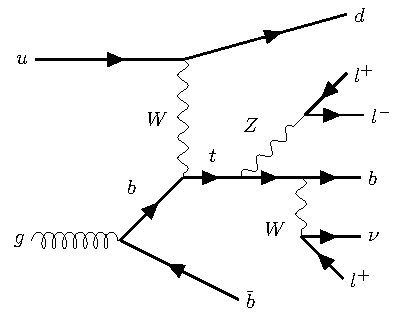
\includegraphics[width=0.7\linewidth]{ubonn-thesis/Chapters/Chapters_05/Figure/tZq_Zfromtop_decay.pdf} 
  \caption{}
  \label{fig:tZq-Zdecay}
  \end{subfigure}%% 
  \begin{subfigure}[b]{0.48\linewidth}
    \centering
    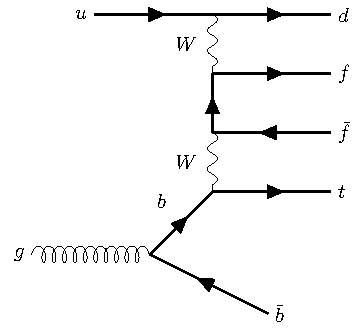
\includegraphics[width=0.7\linewidth]{ubonn-thesis/Chapters/Chapters_05/Figure/tZq_NoZ.pdf} 
  \caption{}
  \label{fig:tZq-nonZdecay}
  \end{subfigure} 
  \caption{Leading order Feynman diagrams with the trilepton final state. (a) resonant production of dilepton pairs, (b) non-resonant production of dilepon pairs }
  \label{fig:tZqdecay}
  \end{figure}


The Feynman diagrams for the trilepton final state at the leading order is shown in figure \ref{fig:tZqdecay}. The signal has also contributions from the non-resonant dilepton production as in figure \ref{fig:tZq-nonZdecay}. The QCD calculations at NLO suggests that there can exist significant QCD radiation present in the event which can manifest itself in the form of a third reconstructed jet. 

In order to increase acceptance as much as reasonably possible two orthogonal signal regions (SRs) named as SR 2j1b and SR 3j1b are defined. In SR 2j1b, events with three leptons, one b-tagged jet and one untagged jet as forward jet are selected. In SR 3j1b, events are selected identically to the SR-2j1b except for the inclusion of a second untagged jet. One of the two untagged jets, that one that gives, with the b-jet, the highest invariant mass, $m_{bj_{f}}$ is selected to be the forward jet. The remaining jet is called radiation jet. The same nomenclature is used for the jets in the control regions (CRs)

\subsection{Full event reconstruction}
\label{sec:event_reconstruction}

From the final states of the process, the variables are reconstructed. The reconstructed variables are the one directly measured in the detector or the intermediate one, calculated from the final state observables.  In order to reconstruct the Z boson, an opposite-sign, same-flavor (OSSF) lepton pair is needed. In the $ee\mu$ and $e\mu\mu$ channels, this is uniquely identified. For the $eee$ and $\mu\mu\mu$ events, both possible combinations are considered and the pair that has the invariant mass closest to the Z boson mass is chosen. 

The remaining lepton and the missing momentum from neutrino is used to reconstruct the W boson. The missing part of the neutrino four-vector is the longitudinal component along the z-axis ($P^{\nu}_{z}$), which can be obtained using the mass constraint of the W boson which is $M_{W}$, 80.4 GeV. The reconstruction technique described below is taken from the ref. \cite{tZq2020}. 
From the four-momentum conservation
\begin{equation}
\label{eqn:four_mom}
   (P^{W})^{2} = ( P^{l} + P^{\nu} )^{2} = M_{W}^{2}
\end{equation}
The solution of the quadratic equation given in eqn. \ref{eqn:four_mom} in terms of the $P^{\nu}_{z}$ can be expressed as follows

\begin{equation}
\label{eqn:pz}
    P^{\nu}_{z} = \frac{\alpha.P^{l}_{z} \pm \sqrt{(E^{l})^{2}( \alpha^{2} - P_{T}^{l}.\cancel{E}_{T}})}{(P^{l}_{T})^{2}}
\end{equation}
where $\alpha$ is given by 
\begin{equation}
\label{eqn:alp}
    \alpha = \frac{M_{W}^{2}}{2} + \overrightarrow{P}^{l}_{T}.\overrightarrow{\cancel{E}}_{T}
\end{equation}
when the quantity under the square root is positive $( \alpha^{2} \geq P_{T}^{l}.\cancel{E}_{T})$, then there are two real solutions, and the smallest one in magnitude is taken. Since the W boson is expected to be produced with small rapidity. For some events, eqn. \ref{eqn:four_mom} has imaginary solution $( \alpha^{2} \leq P_{T}^{l}.\cancel{E}_{T})$, which is interpreted as a mis-measurement of $\cancel{E}_{T}$. In this case the transverse mass, $m_{T}(W)$, is greater than $M_{W}$ and $m_{T}(W)$ is explicitly set to equal $M_{W}$ and the neutrino 4-vector is rescaled. Technically this is resolved by introducing a new scale factor $\beta$, which is defined by 
\begin{equation}
\label{eqn:beta}
    \beta = \frac{M_{W}^{2}}{2P^{l}_{T}}.\cancel{E}_{T} - \overrightarrow{P}^{l}_{T}.\overrightarrow{\cancel{E}}_{T}
\end{equation}
$\beta$ is used to scale $\cancel{E}_{x}$, $\cancel{E}_{y}$ and $\cancel{E}_{T}$ and then $\alpha$ is recalculated as shown in eqn. \ref{eqn:alp}. $P^{\nu}_{z}$ is found by considering only the offset part of the eqn. \ref{eqn:pz}.

Then, the reconstructed W boson and the b-tagged jet are used for the t-quark reconstruction as follows
\begin{equation}
\label{eqn:top}
    P^{t} = P^{W} + P^{b\text{-}jet}
\end{equation}
A summary of relevant symbols representing the reconstructed objects is presented in table \ref{tab:reco}

\begin{table}[h!]
\centering
 \begin{tabular}{@{} *2l @{}}
 \toprule
 Symbol & Description   \\ [0.5ex] 
 \hline\hline 
  $l^{1}_{Z}$ & Highest $p_{T}$ lepton from the reconstructed Z boson \\ [0.5ex] 
  $l^{2}_{Z}$ & Lowest $p_{T}$ lepton from the reconstructed Z boson \\ [0.5ex] 
  Z & Reconstructed Z boson \\ [0.5ex]
  $l_{W}$ & Lepton from the reconstructed W boson from the t-quark decay \\ [0.5ex]
  W & Reconstructed W boson from the t-quark decay \\ [0.5ex]
 b-jet & b-tagged jet \\ [0.5ex]
 t & Reconstructed t quark \\ [0.5ex]
 $j_{f}$ & Forward jet  \\ [0.5ex]
 $j_{r}$ & Radiation jet \\ [0.5ex]
 \hline
$l_{1/2/3}$ & $p_{T}$ ordered leptons \\ [0.5ex]
$j_{1/2/3}$ & $p_{T}$ ordered jets \\ [0.8ex]
 \bottomrule
 \end{tabular}
 \caption{Object reconstruction.}
 \label{tab:reco}
\end{table}



\subsection{Lepton isolation working point}
\label{subsec:LWP}

In order to reduce the contribution of the background processes from the non-prompt leptons, the isolation working points are studied. For details on isolation working point ref. \cite{isolationwp:2010n} can be referred. 
\begin{table}[h!]
\centering
 \begin{tabular}{@{} *5l @{}}
 \toprule
 Name & Electron & Muon  \\ [0.5ex] 
 \hline\hline
 Gradient & Gradient & FCTightTrackOnly$\_$FixedRad  \\ 
 PLV & PLVTight & PLVTight  \\
 PLVLoose & PLVLoose & PLVLoose \\
 PLIV & PLImprovedTight & PLImprovedTight  \\
 PLIVV & PLImprovedVeryTight & PLImprovedVeryTight  \\
 Pflow & PflowTight & PflowTight$\_$VarRad  \\
 TrackOnly & TightTrackOnly &  TightTrackOnly$\_$VarRad \\
 Tight & Tight & Tight$\_$VarRad  \\ [1ex] 
 \bottomrule
 \end{tabular}
 \caption{Combination of the isolation working point analysed}
 \label{tab:lep_wp}
\end{table}

\begin{figure}[h!]
    \centering
    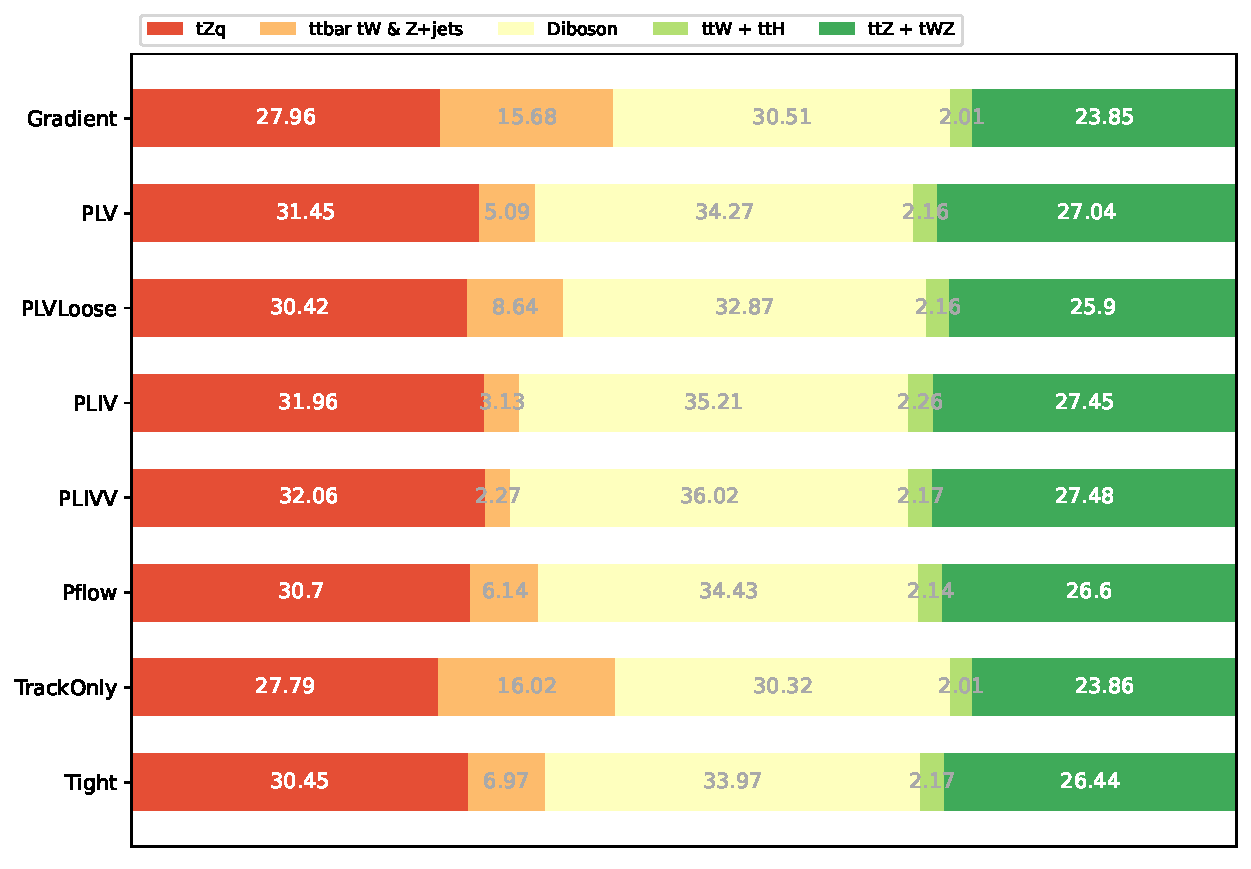
\includegraphics[width=0.85\textwidth]{ubonn-thesis/Chapters/Chapters_05/Figure/Lepton WPs/percent_plt_2j1b.pdf}
    \caption{Relative yield for SR 2j1b with jet $p_{T} > 35$ GeV, lepton $p_{T} >$ 28, 20, 20 , GeV \& btag-eff: 70\%}
    \label{fig:lep_wp_2j1b}
\end{figure}
 
\begin{figure}[h!]
    \centering
    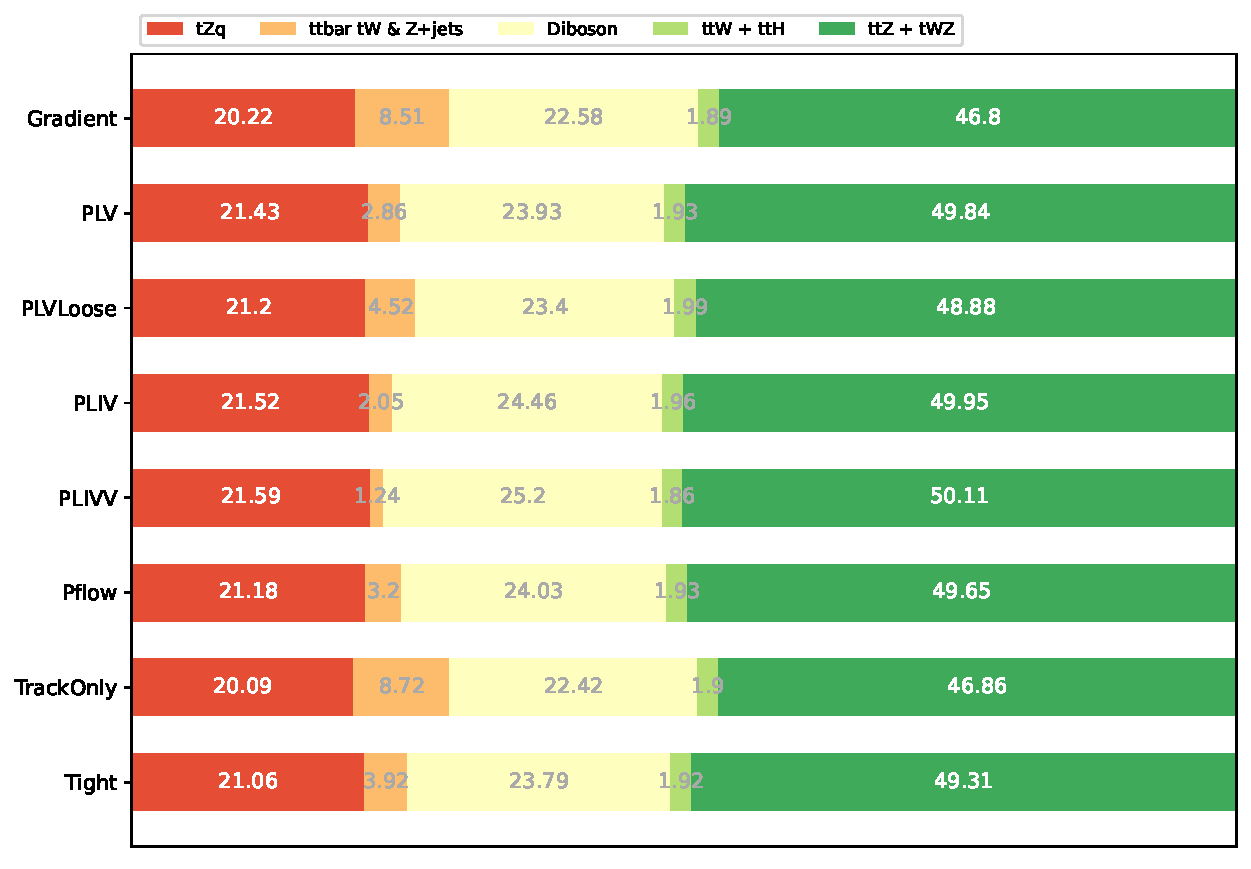
\includegraphics[width=0.85\textwidth]{ubonn-thesis/Chapters/Chapters_05/Figure/Lepton WPs/percent_plt_3j1b.pdf}
    \caption{Relative yield for SR 3j1b with jet $p_{T} > 35$ GeV, lepton $p_{T} >$ 28, 20, 20 , GeV \& btag-eff: 70\%}
    \label{fig:lep_wp_3j1b}
\end{figure}


In this analysis, the yield for a set of isolation WPs shown in the table \ref{tab:lep_wp} is presented. The yield are obtained with the following selection cuts: The three leptons are sorted by their $p_{T}$, irrespective of flavour, and required to have transverse momenta of at least 28, 20 and 20 GeV, respectively. Jets are required to have $P_{T} > 35$ GeV with one b-tagged jet with 70\% WP.


 Figures \ref{fig:lep_wp_2j1b} and \ref{fig:lep_wp_3j1b} show the relative yield for the different lepton WPs.  It is found that PLV, PLIV, and PLIVV have large signal and small fake-background compared to others. While PLVLoose has comparatively large fake background. The significance calculated in table \ref{tab:WP_sig} shows that PLVLoose has the highest significance for both SR-2j1b and SR-3j1b. The significance is also high for PLV and PLIV compared  to others. So, the lepton WPs: PLV, and PLVLoose are chosen for the optimization of selection cuts. 
 
\begin{table}[h!]
\centering
\begin{tabular}{@{} *8l  @{}}
\toprule
 & \multicolumn{3}{c}{SR 2j1b} & \multicolumn{3}{c}{SR 3j1b} \\
 \midrule
Lepton WPs & S & B & $\frac{S}{\sqrt{S+B}}$ & S & B & $\frac{S}{\sqrt{S+B}}$  \\ [0.2cm]
\toprule
 Gradient & 89.40 & 230.38 & 5.00 & 50.89 & 200.73 &  3.21  \\

PLV  & 83.73 & 182.51 &  5.13 & 47.67 & 174.82 &  3.20 \\ 

PLVLoose  & 91.50 & 209.26 &  5.28 & 52.10 & 193.61 &  3.32 \\

PLIV  & 80.70 & 171.8 &  5.08 & 46.10 & 168.10 &  3.15 \\ 

PLIVV  & 66.50 & 140.90 &  4.62 & 38.30 & 139.10 &  2.88 \\ 

Pflow & 79.86 & 180.27 & 4.95  & 45.79 & 170.38 & 3.11 \\

TrackOnly & 92.59 & 240.56 &  5.07 & 52.61 & 209.22 & 3.25 \\

Tight & 81.82 & 186.88 & 4.99 & 46.96 & 176.06 & 3.14  \\
\bottomrule
\end{tabular}
\caption{Values of the Significance for SR 2j1b and SR 3j1b for various isolation WPs}
\label{tab:WP_sig}
\end{table}  

%\newpage

%\newpage

\subsection{Optimization of cuts}
\label{subsec:Opti_cuts}

The analysis aims to set new requirements on the phase space so that the contribution of the signal grows relative to the number of background events. The significance is calculated for different selection cuts and are compared to the previous selections used in ref. \cite{tZq2020}. The cuts are optimized by varying leptons $p_{T}$, jets $p_{T}$ and the b-tagging efficiency of the b-tagged jet. The analysis framework uses the leptons sorted in $p_{T}$ ordered.

\vspace*{-0.2cm}
\begin{figure}[h!] 
  \begin{subfigure}[b]{0.49\linewidth}
    \centering
    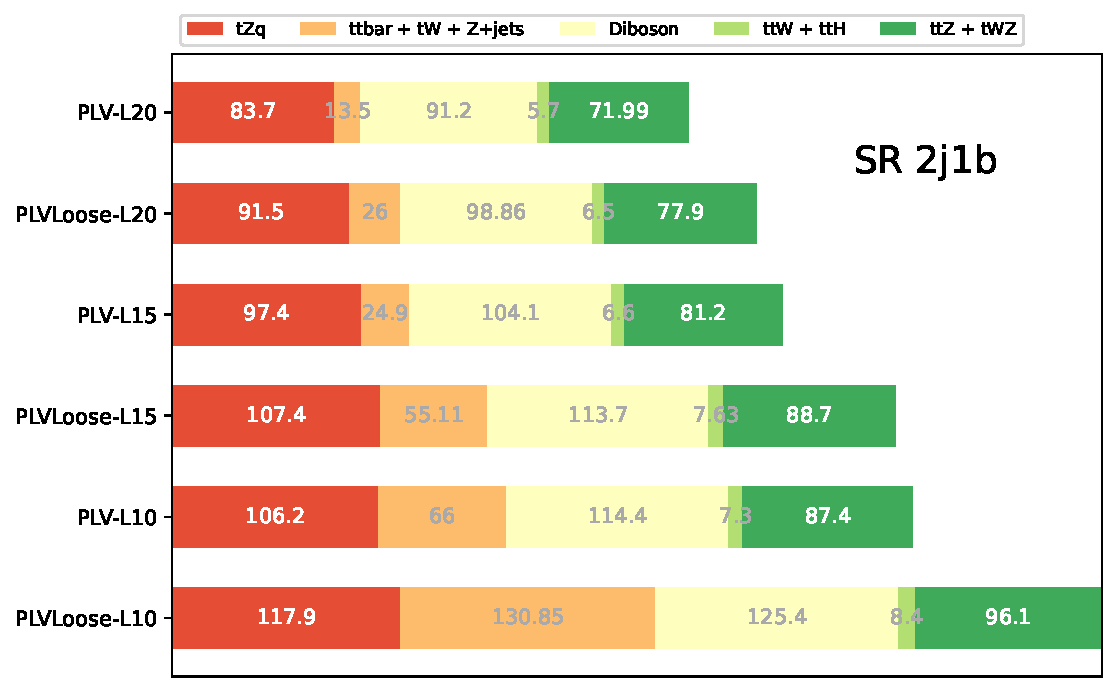
\includegraphics[width=\linewidth]{ubonn-thesis/Chapters/Chapters_05/Figure/Cuts Optimization/SR2j1b_PLVLoose.pdf}
    \end{subfigure}%% 
  \begin{subfigure}[b]{0.49\linewidth}
    \centering
    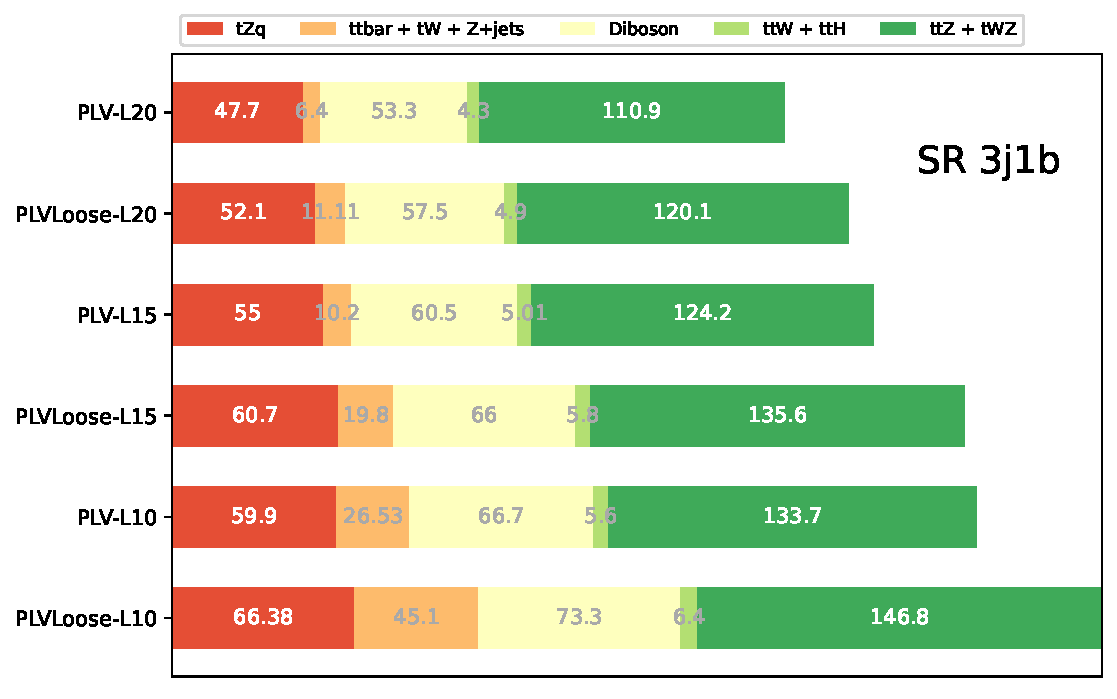
\includegraphics[width=\linewidth]{ubonn-thesis/Chapters/Chapters_05/Figure/Cuts Optimization/SR3j1b_PLVLoose.pdf} 
  \end{subfigure} 
  \vspace*{-0.2cm}
  \caption{Yield for signal and background at varying third lepton $p_{T}$ }
  \label{fig:third_lep}
  \end{figure}

\vspace*{-0.2cm}
\begin{table}[h!]
\centering
\begin{tabular}{@{} *8l  @{}}
\toprule
& & \multicolumn{3}{c}{SR 2j1b}  & \multicolumn{3}{c}{SR 3j1b}\\ 
 \midrule
Lepton WPs & $p_{T}(\ell_3) > $ & S & B & $\frac{S}{\sqrt{S+B}}$   & S & B & $\frac{S}{\sqrt{S+B}}$\\ [0.2cm]
\toprule
 \multirow{3}{*}{PLV} & $ \SI{20}{\GeV}$ & 83.70 & 182.39 &  5.13  & 47.7 & 174.9 &  3.20  \\

  & $ \SI{15}{\GeV}$ & 97.40 & 216.80 & 5.49 & 55.00 & 199.91 & 3.44  \\ 

 & $ \SI{10}{\GeV}$ & 106.40 & 275.10  & 5.45  & 59.90 & 232.53  & 3.50  \\
\midrule
 \multirow{3}{*}{PLVLoose} & $ \SI{20}{\GeV}$ & 91.50 & 209.26 & 5.28 & 52.10 & 193.61 & 3.32  \\

  & $ \SI{15}{\GeV}$ & 107.40 &  265.14 & 5.56 & 60.7 &  227.20 & 3.58  \\ 

 & $ \SI{10}{\GeV}$ & 117.90 & 360.75  & 5.35 & 66.38 & 271.60  & 3.61    \\
\bottomrule
\end{tabular}
\vspace*{-0.1cm}
\caption{Significance calculated at varying third lepton $p_{T}$ for both SR 2j1b and SR 3j1b}
\label{tab:third_lep_opt}
\end{table}

Figure \ref{fig:third_lep} shows the yield at varying third lepton $p_{T}$, while the first and third lepton lepton $p_{T}$ remain at 28 GeV and 20 GeV respectively. The btagging WP is 70\% and the jet transverse momentum remain above 30 GeV. It shows that both the signal and background increases with loose third lepton $p_{T}$ cut. The significance in table \ref{tab:third_lep_opt} that PLV at 10 GeV and PLVLoose at 15 GeV have considerable signal to background ratio while significance is above $5 \sigma$ for SR 2j1b and $3 \sigma$ for SR 3j1b. Figure \ref{fig:first_second_lepton_pt} shows that the change in the first lepton $p_{T}$ from 28 GeV to 27 GeV doesnot change the yield much for both PLV and PLVLoose. Similarly the yield remains same by changing the second lepton $p_{T}$ from 20 GeV to 15 GeV. Thus the final cut for analysis for the leptons $p_{T}$ are set to 27, 20, 10 GeV for PLV and 27, 20, 15 GeV for PLVLoose for first, second and third lepton $p_{T}$ respectively.

\begin{figure}[h!] 
  \begin{subfigure}[b]{0.49\linewidth}
    \centering
    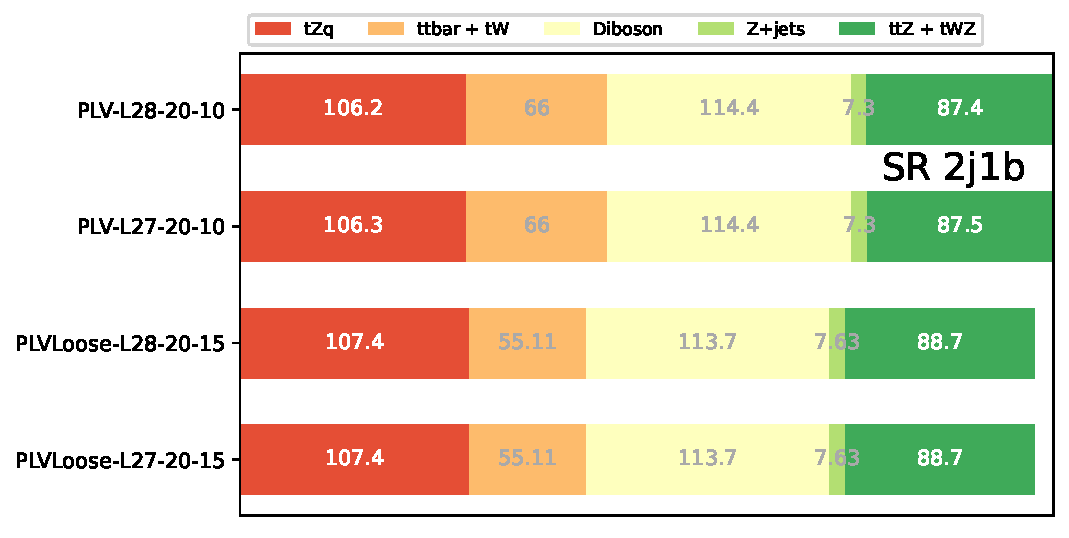
\includegraphics[width=\linewidth]{ubonn-thesis/Chapters/Chapters_05/Figure/Cuts Optimization/SR2j1b_PLVLoose_27.pdf} 
  \end{subfigure} 
  \hfill
  \begin{subfigure}[b]{0.49\linewidth}
    \centering
    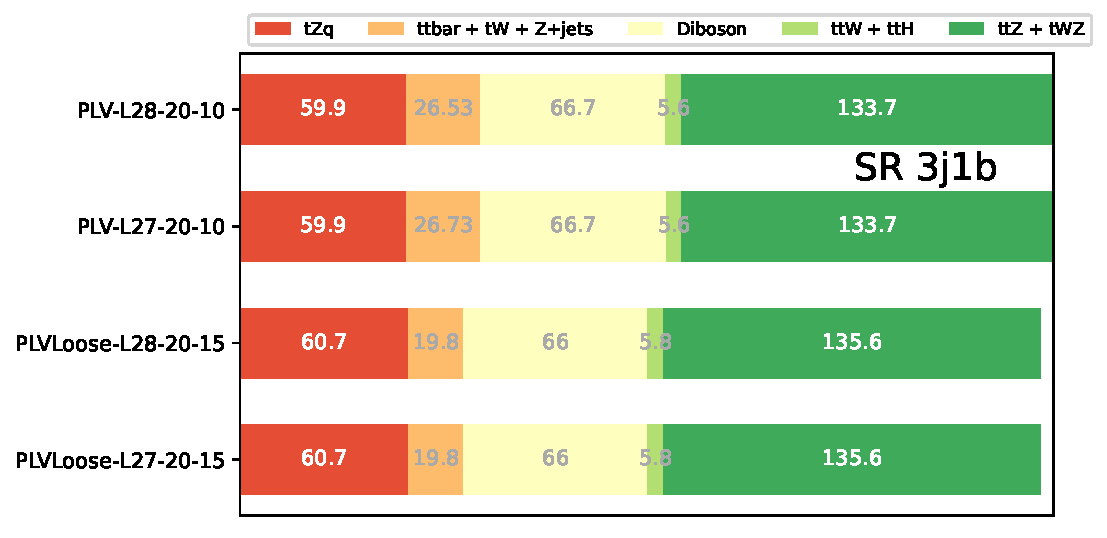
\includegraphics[width=\linewidth]{ubonn-thesis/Chapters/Chapters_05/Figure/Cuts Optimization/SR3j1b_PLVLoose_27.pdf} 
  \end{subfigure} 
  \caption{Events yield for signal and background at varying first lepton $p_{T}$ }
  \end{figure}
  \begin{figure}[h!] 
  \begin{subfigure}[b]{0.49\linewidth}
    \centering
    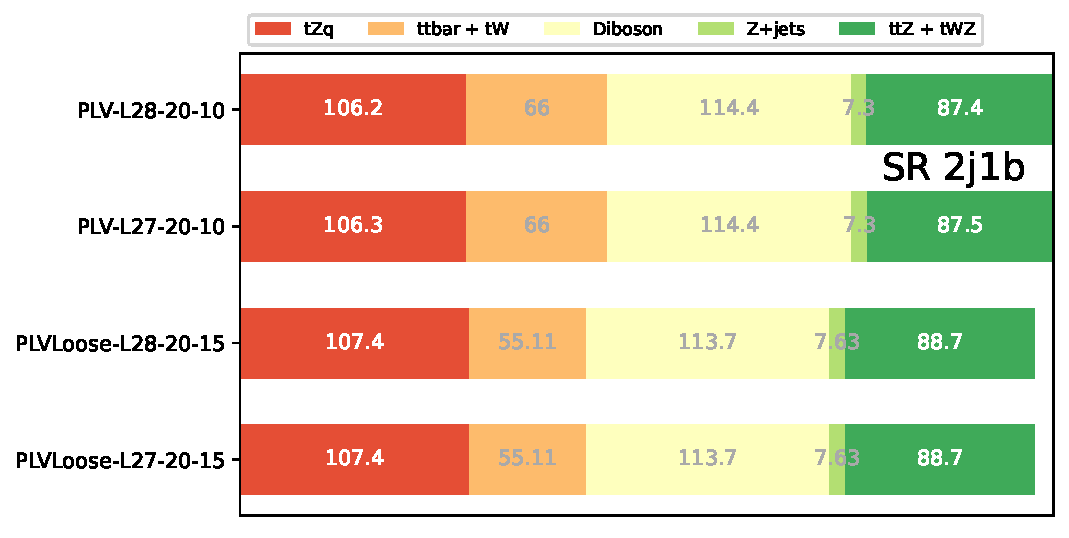
\includegraphics[width=\linewidth]{ubonn-thesis/Chapters/Chapters_05/Figure/Cuts Optimization/SR2j1b_PLVLoose_27.pdf} 
  \end{subfigure} 
  \hfill
  \begin{subfigure}[b]{0.49\linewidth}
    \centering
    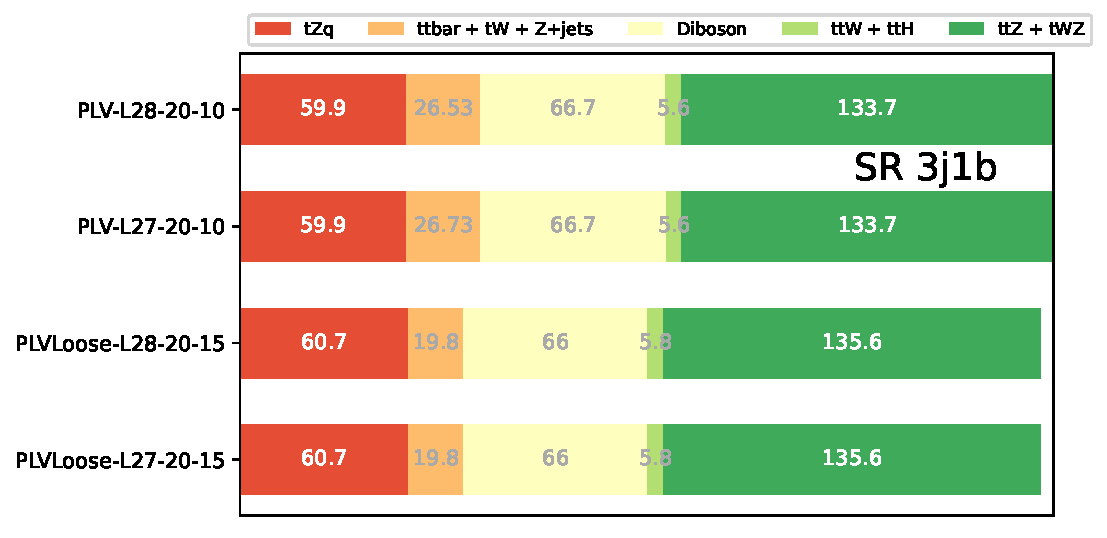
\includegraphics[width=\linewidth]{ubonn-thesis/Chapters/Chapters_05/Figure/Cuts Optimization/SR3j1b_PLVLoose_27.pdf} 
  \end{subfigure} 
  \caption{Events yield for signal and background at varying second lepton $p_{T}$}
  \label{fig:first_second_lepton_pt}
  \end{figure}
 
Figures \ref{fig:SR_2j1bbtag} and \ref{fig:SR_3j1btag} show the yield at varying jet $p_{T}$, b-tagging efficiency and third lepton $p_{T}$. The lower in jet $p_{T}$ migrate the signal to higher jet multiplicity keeping total number of signal in SR 2j1b and SR 3j1b nearly same. There is large increase in diboson background yield with increase in b-tagging working point. Here, in the plot the diboson contribution is split according to the origin of the associated jets using generator-level information. If one of the jets contains a b- or c-hadron then it is classified as diboson + heavy flavour (VV + HF), otherwise the event is classified as diboson + light flavour (VV + LF). Thus for final cut for the jet transverse momentum and b-jet tagging efficiency for our analysis remain at 35 GeV and 70\%. 

\begin{figure}[h!]
    \centering
    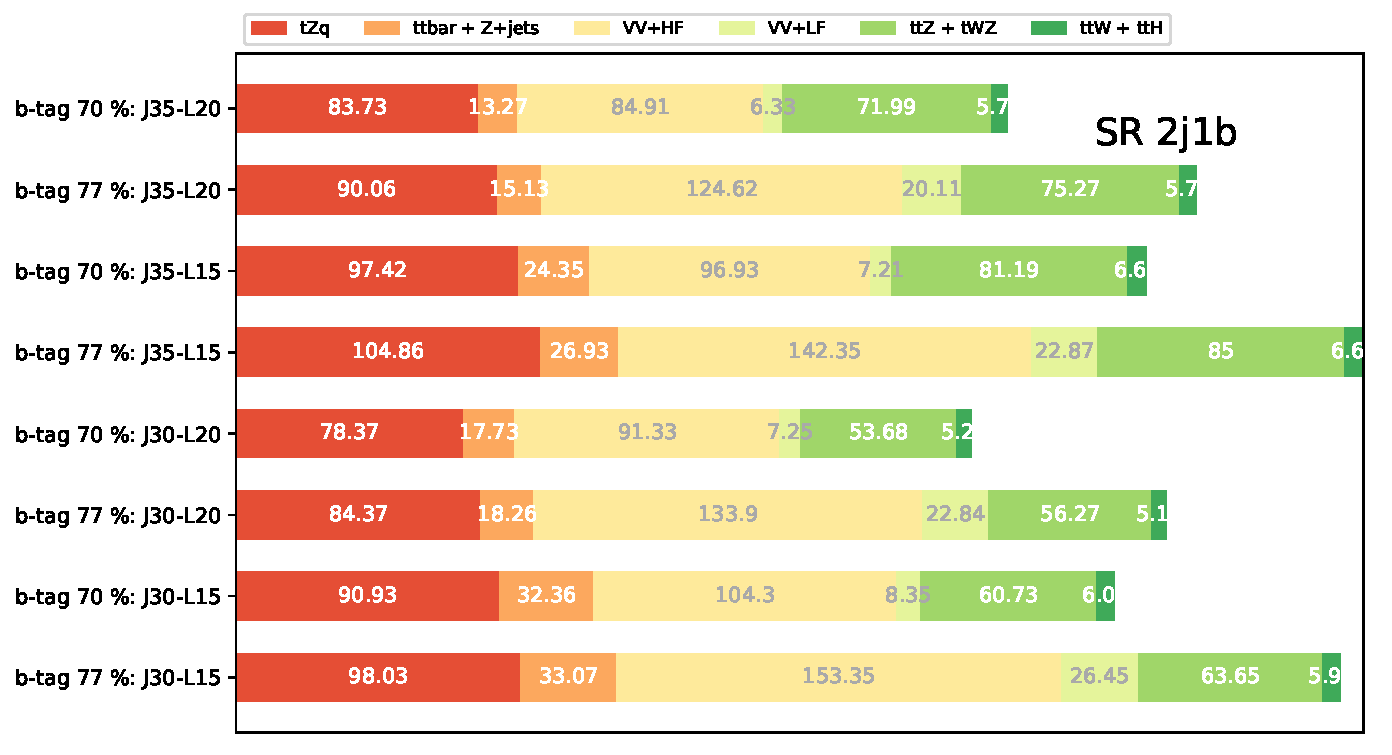
\includegraphics[width=0.75\textwidth]{ubonn-thesis/Chapters/Chapters_05/Figure/Cuts Optimization/jet_2j1b_yield.pdf}
    \caption{Events yeild for signal and background obtained by varing the jet $p_{T}$, b-tagging efficiency and the third lepton $p_{T}$ in the SR 2j1b}
    \label{fig:SR_2j1bbtag}
\end{figure}

\begin{figure}[h!]
    \centering
    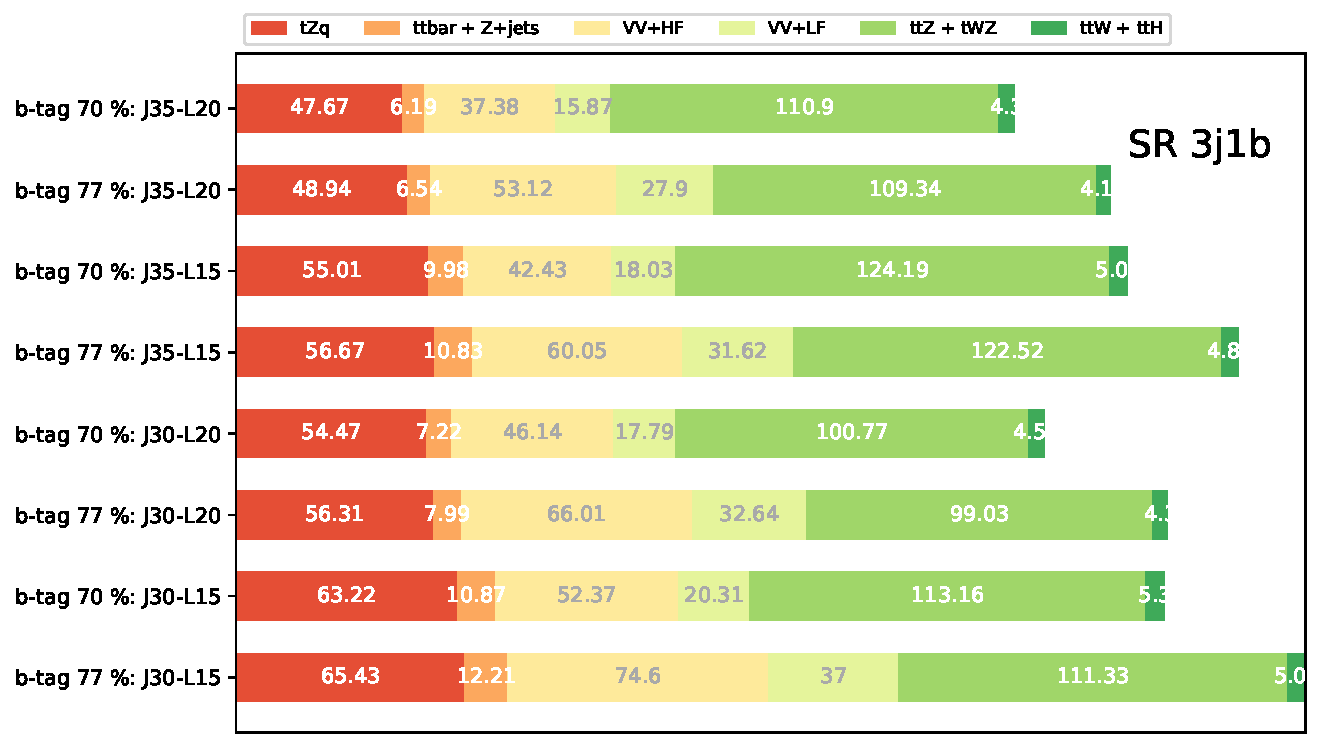
\includegraphics[width=0.75\textwidth]{ubonn-thesis/Chapters/Chapters_05/Figure/Cuts Optimization/jet_3j1b_yield.pdf}
    \caption{Events yeild for signal and background obtained by varing the jet $p_{T}$, b-tagging efficiency and the third lepton $p_{T}$ in the SR 3j1b}
    \label{fig:SR_3j1btag}
\end{figure}



\subsection{Signal regions (SRs) plots and yields}
\label{subsec:SR_plot_yield}

The regions are constructed as described in section \ref{sec:SR}. The full selection cuts applied in the signal regions are listed in table \ref{tab:final_selection}. In this table, the selection cuts for the definition of control regions are  

\begin{table}[hbt!]
\centering
\begin{tabular}{@{} *4l  @{}}
\toprule
& \multicolumn{2}{c}{Common selections} & \\
\midrule
& \multicolumn{2}{c}{Exactly 3 leptons ($e$ or $\mu$) with $|\eta| < 2.5$} &  \\
& \multicolumn{2}{c}{$p_{T}(\ell_1)> \SI{27}{\GeV}$, $p_{T}(\ell_2)> \SI{20}{\GeV}$, $p_{T}(\ell_3)> \SI{10}{\GeV}$} &  \\
& \multicolumn{2}{c}{$p_{T}(\text{jet})> \SI{35}{\GeV}$} &  \\[0.3em]
\toprule
SR 2j1b  & CR Diboson 2j0b & CR $t\Bar{t}Z$ 3j2b & CR $t\Bar{t}$ 2j1b  \\
\midrule
$\ge$ 1 OSSF pair & $\ge$ 1 OSSF pair & $\ge$ 1 OSSF pair & $\ge$ 1 OSDF pair  \\
$|m_{\ell \ell} - m_{Z}| <  \SI{10}{\GeV}$ & $|m_{\ell \ell} - m_{Z}| < $ \SI{10}{\GeV} & $|m_{\ell \ell} - m_{Z}| < $ \SI{10}{\GeV} & No OSSF pair  \\
2 jets, $|\eta| < $ 4.5  & 2 jets, $|\eta| < $ 4.5  & 3 jets, $|\eta| < $ 4.5 & 2 jets, $|\eta| < $ 4.5  \\
1 bjet, $|\eta| < $ 2.5 & 0 bjets & 2 bjets, $|\eta| < $ 2.5  & 1 bjet, $|\eta| < $ 2.5   \\[0.3em]
\toprule
SR 3j1b   & CR Diboson 3j0b & CR $t\Bar{t}Z$ 4j2b & CR $t\Bar{t}$ 3j1b \\
\midrule
$\ge$ 1 OSSF pair & $\ge$ 1 OSSF pair & $\ge$ 1 OSSF pair & $\ge$ 1 OSDF pair \\
$|m_{\ell \ell} - m_{Z}| <  \SI{10}{\GeV}$ & $|m_{\ell \ell} - m_{Z}| < $ \SI{10}{\GeV} & $|m_{\ell \ell} - m_{Z}| < $ \SI{10}{\GeV} & No OSSF pair  \\
3 jets, $|\eta| < $ 4.5  & 3 jets, $|\eta| < $ 4.5  & 4 jets, $|\eta| < $ 4.5 & 3 jets, $|\eta| < $ 4.5  \\
1 bjet, $|\eta| < $ 2.5 & 0 bjets  & 2 bjets, $|\eta| < $ 2.5  & 1 bjet, $|\eta| < $ 2.5   \\
\bottomrule
\end{tabular}
\caption{Overview of the requirements applied when selecting events in the signal and control regions. OSSF is an opposite-sign same-flavour lepton pair. OSDF is an opposite-sign different-flavour lepton pair.}
\label{tab:final_selection}
\end{table}
 
also reported. The event yields in the SRs after the full selection can be found in table \ref{tab:yield_SR} and histogram distributions of reconstructed variables from the top quark and Z boson are given in figure \ref{fig:signal}. The predicted number of events to pass selection cuts based on MC simulations for tZq as well as all previously mentioned backgrounds are tabulated. The events in these regions are the primary regions of interest for the statistical analysis described in section \ref{sec: Profile_likehihood} after having been evaluated by the neural network described in section \ref{sec:NN}.

\begin{table}[!h]
    \begin{minipage}{.49\textwidth}
      \centering
      \begin{adjustbox}{width=\textwidth}
       \begin{tabular}{@{} *3l @{}}
 \toprule
 Process & Number of events & Number of raw events  \\ [0.5ex] 
 \hline\hline
  tZq   & 97.46 \pm 0.67 & 56838800 \\ 
  tt   & 22.72 \pm 0.88  & 104389 \\ 
  tW   & 0.89 \pm 0.61   & 1112 \\ 
  Z+jets   & 36.66 \pm 4.13 & 228516 \\ 
  Diboson   & 115.60 \pm 1.09  & 5741400 \\ 
  ttZ   & 62.88 \pm 2.30 & 7001290  \\ 
  ttW   & 4.56 \pm 0.18 & 255621  \\ 
  tWZ   & 19.34 \pm 0.58 & 489419 \\ 
  ttH   & 2.11 \pm 0.04   & 715711 \\ 
\hline 
  Total expected  & 362.22 \pm 4.65 & 71376200 \\ 
\hline 
  Data   & 443  & 443  \\   
 \bottomrule
 \end{tabular} 
 \end{adjustbox}
    \end{minipage}%
    \hfill
    %\hspace{-1.5cm}
    \begin{minipage}{.49\textwidth}
      \centering
      \vspace*{0.5cm}
      \begin{adjustbox}{width=\textwidth}
        \begin{tabular}{@{} *3l @{}}
 \toprule
 Process & Number of events & Number of raw events  \\ [0.5ex] 
 \hline\hline
   tZq   &  55.31 \pm 0.56 & 38569200 \\ 
  tt   & 10.79 \pm 0.61 & 49206 \\ 
  tW   & 0.33 \pm 0.58 & 417 \\ 
  Z+jets & 13.32 \pm 1.14 & 102582 \\ 
  Diboson  & 66.05 \pm 0.70 & 3615390 \\ 
  ttZ   & 101.39 \pm 0.68 & 12441100 \\ 
  ttW   & 2.34 \pm 0.13 & 134969 \\ 
  tWZ   & 22.92 \pm 0.65 & 596449 \\ 
  ttH   & 2.80 \pm 0.05  & 753658 \\ 
\hline 
  Total expected  & 275.24 \pm 1.84 & 56262900 \\ 
\hline 
  Data    & 307 & 307 \\ 
 \bottomrule
 \end{tabular} 
 \end{adjustbox}
\end{minipage} 
\caption{Numbers of expected events in the SR 2j1b (Left) and SR 3j1b (Right) broken down by process. The uncertainty shown contains only the statistical component.}
\label{tab:yield_SR}
\end{table}


\begin{figure}[h!] 
  \begin{subfigure}[b]{0.33\linewidth}
    \centering
    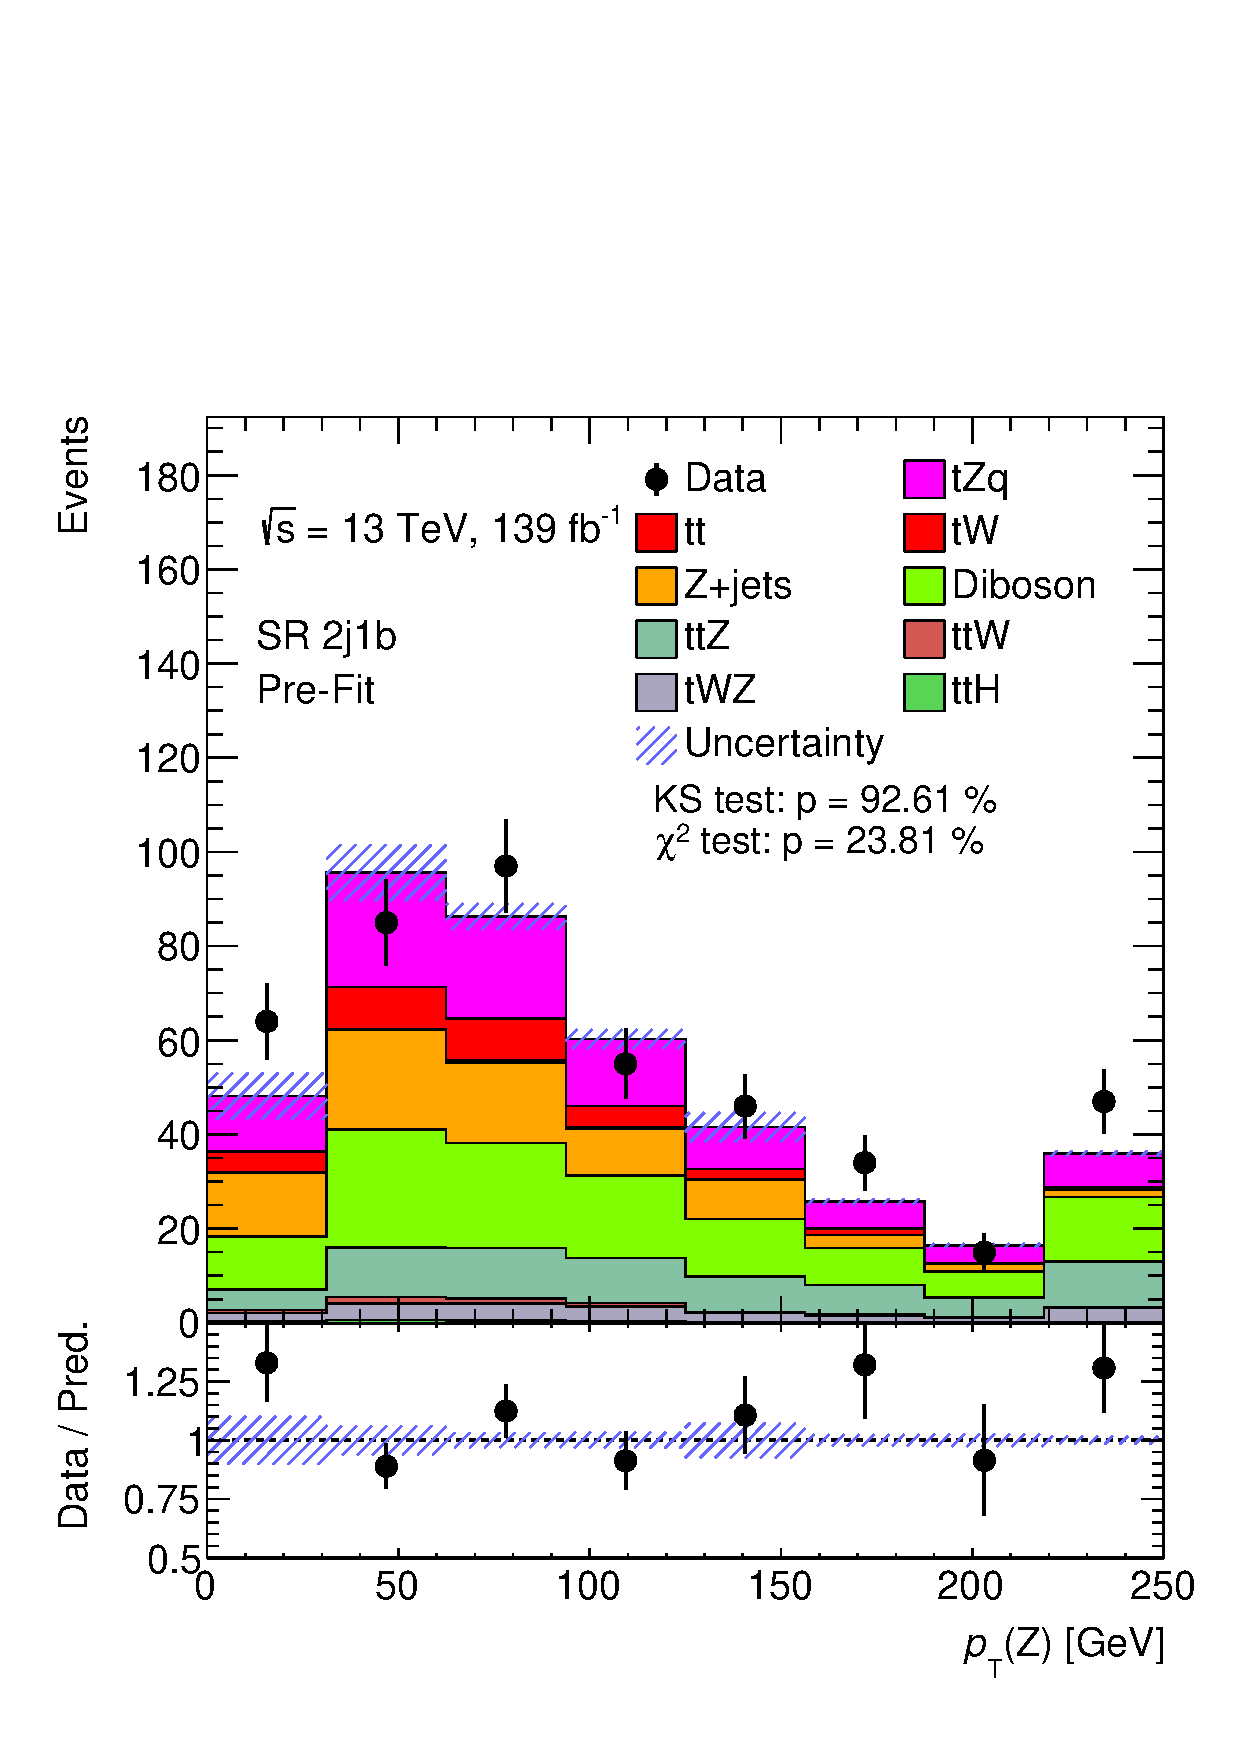
\includegraphics[width=\linewidth]{ubonn-thesis/Chapters/Chapters_05/Figure/SR/SR_2j1b_Z_pt.pdf} 
  \end{subfigure}%% 
  \begin{subfigure}[b]{0.33\linewidth}
    \centering
    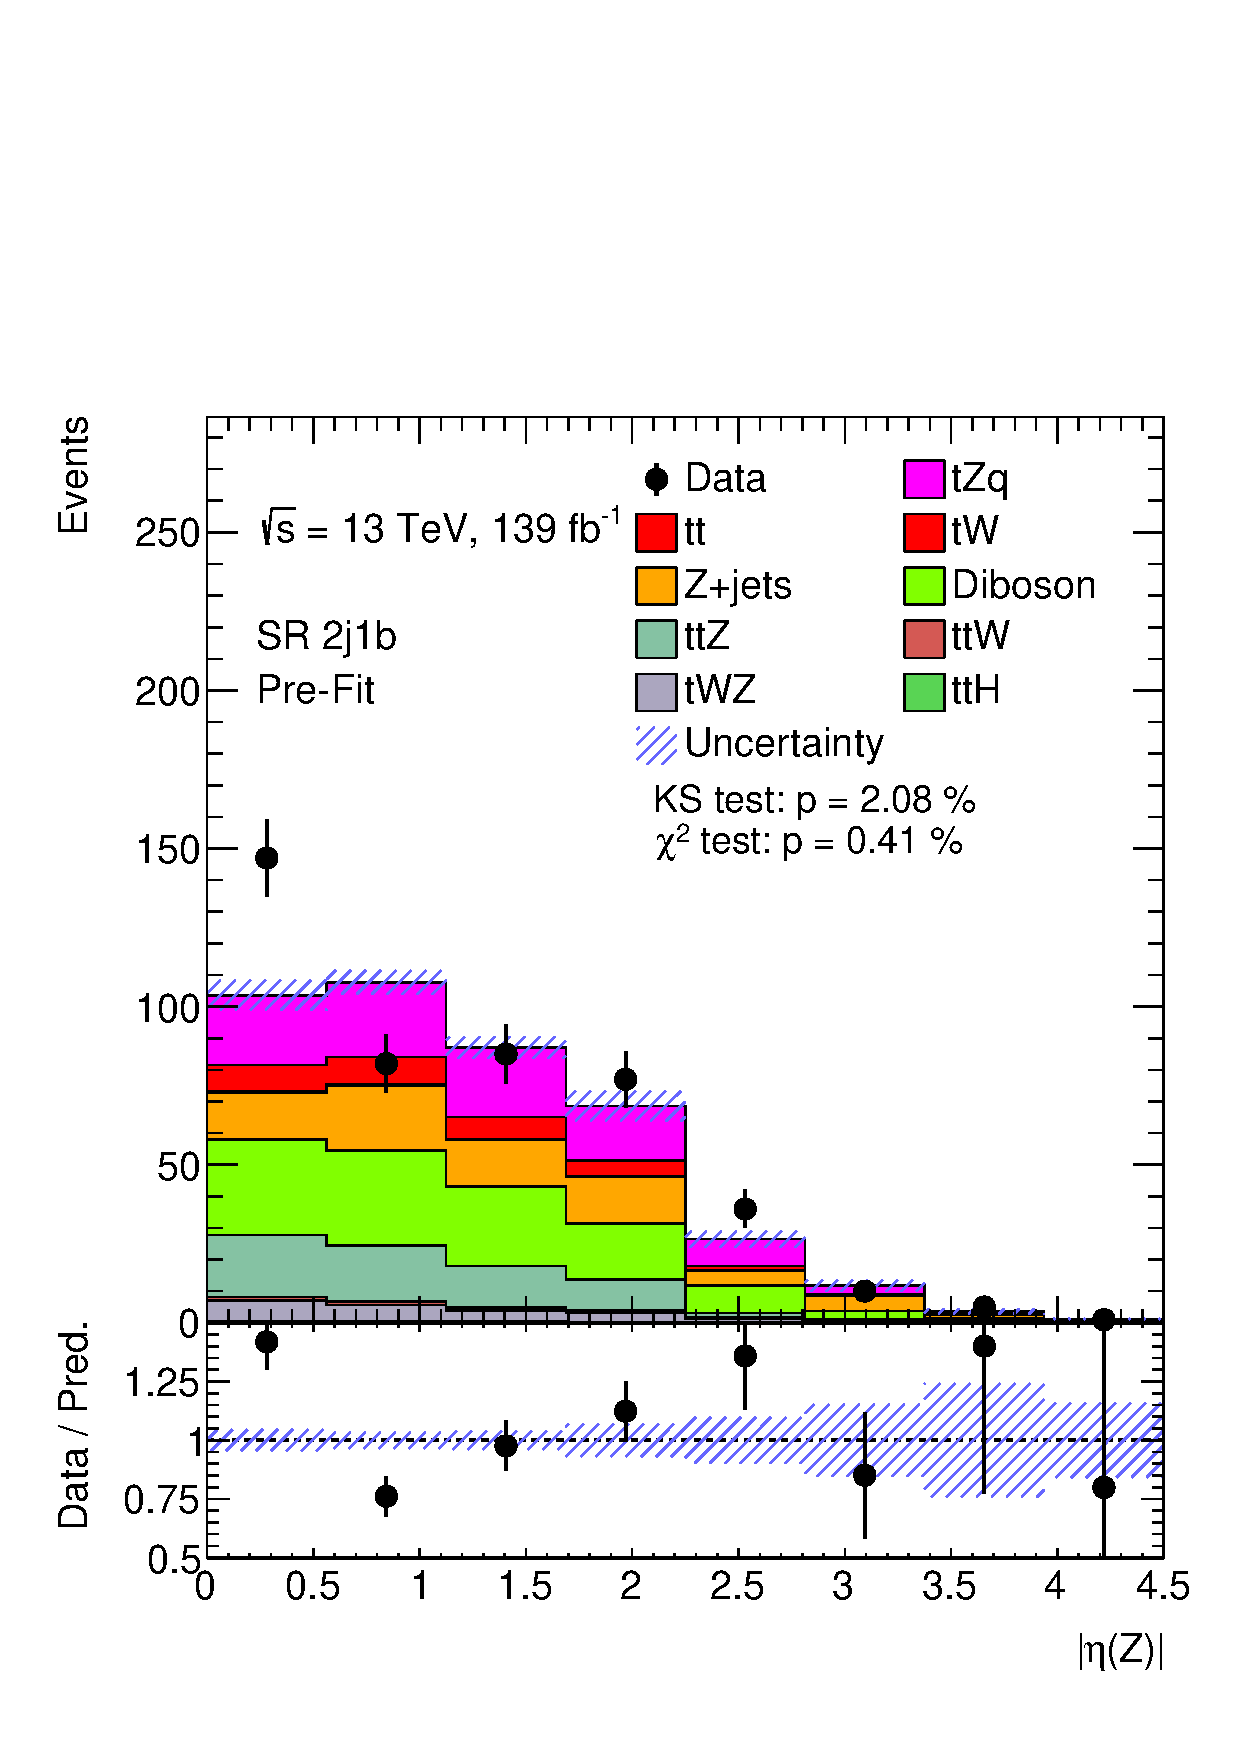
\includegraphics[width=\linewidth]{ubonn-thesis/Chapters/Chapters_05/Figure/SR/SR_2j1b_Z_eta.pdf} 
  \end{subfigure} 
  \begin{subfigure}[b]{0.33\linewidth}
    \centering
    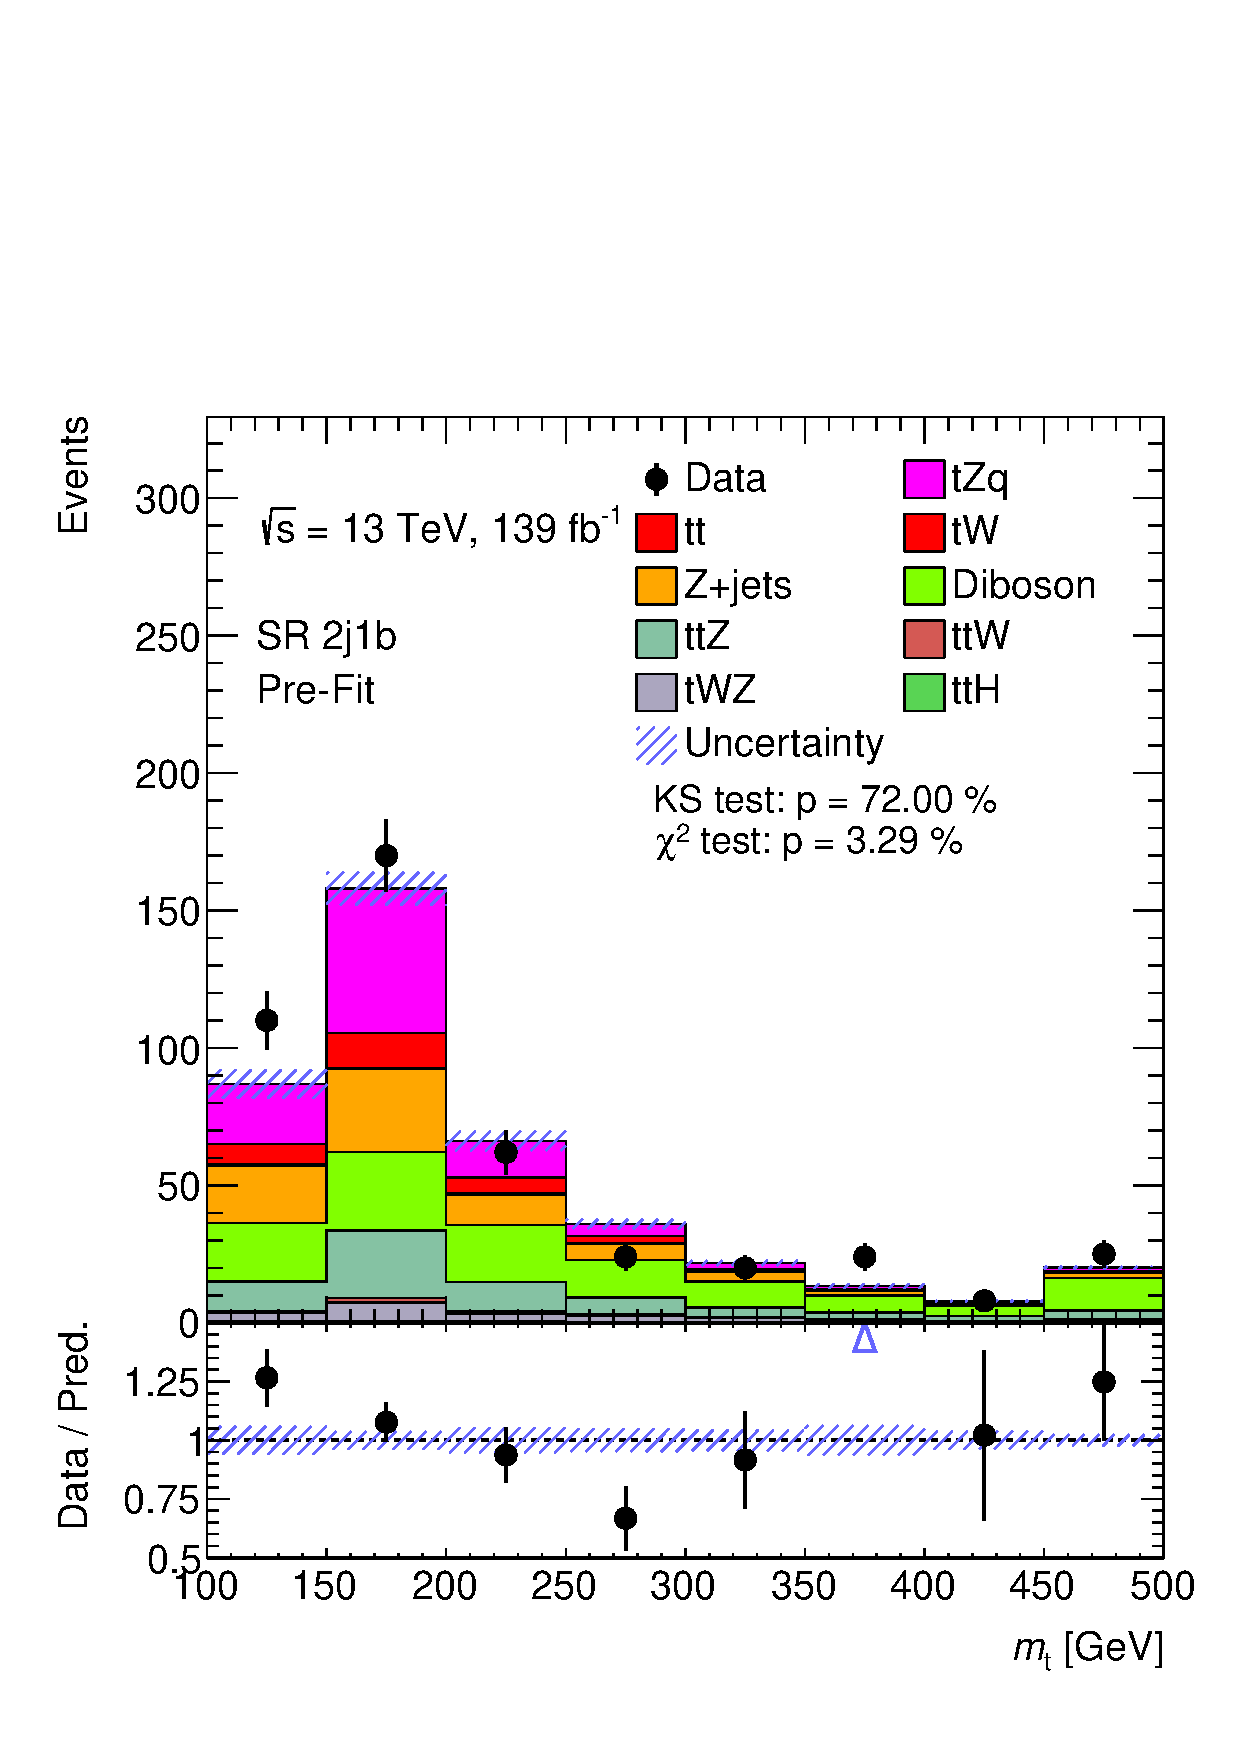
\includegraphics[width=\linewidth]{ubonn-thesis/Chapters/Chapters_05/Figure/SR/SR_2j1b_Top_mass.pdf} 
  \end{subfigure}%%
  \newline
  \begin{subfigure}[b]{0.33\linewidth}
    \centering
    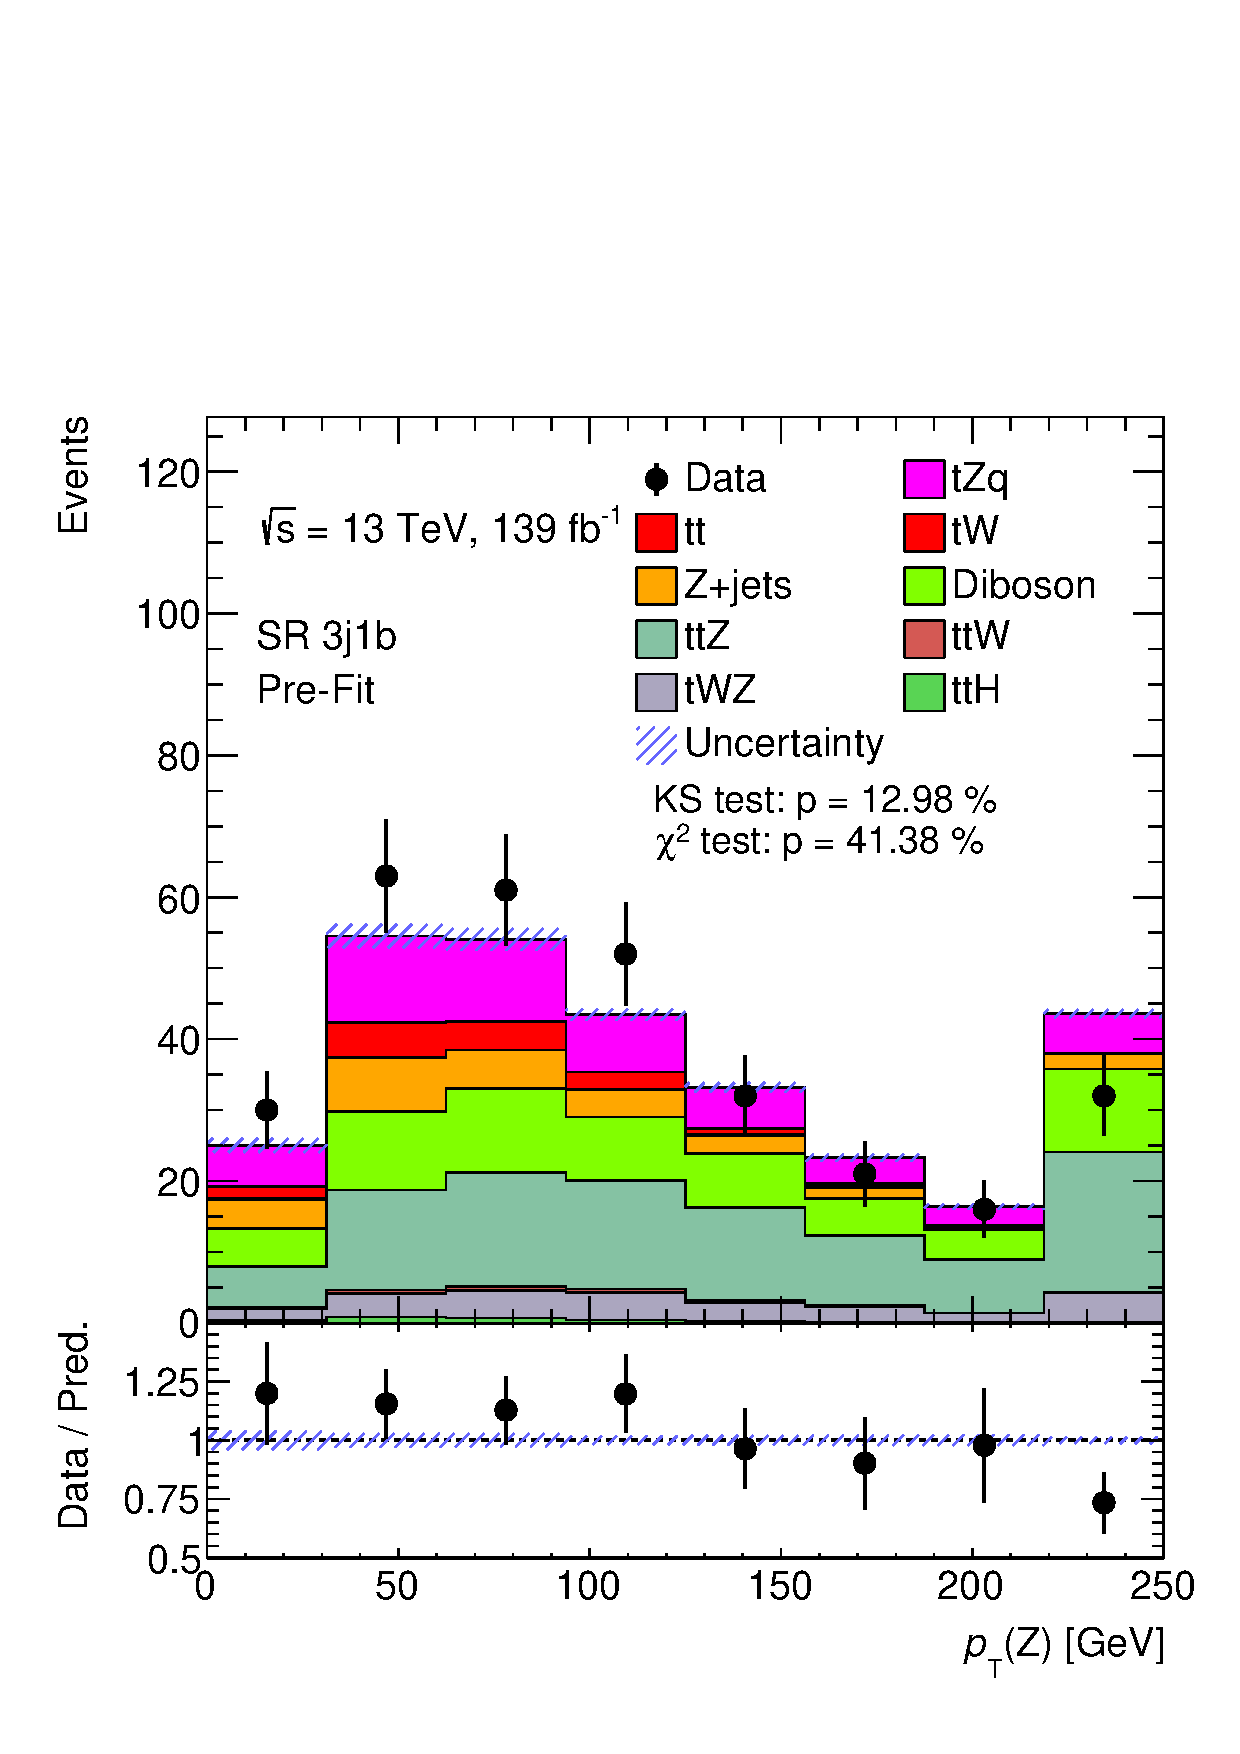
\includegraphics[width=\linewidth]{ubonn-thesis/Chapters/Chapters_05/Figure/SR/SR_3j1b_Z_pt.pdf} 
  \end{subfigure}%%
  \begin{subfigure}[b]{0.33\linewidth}
    \centering
    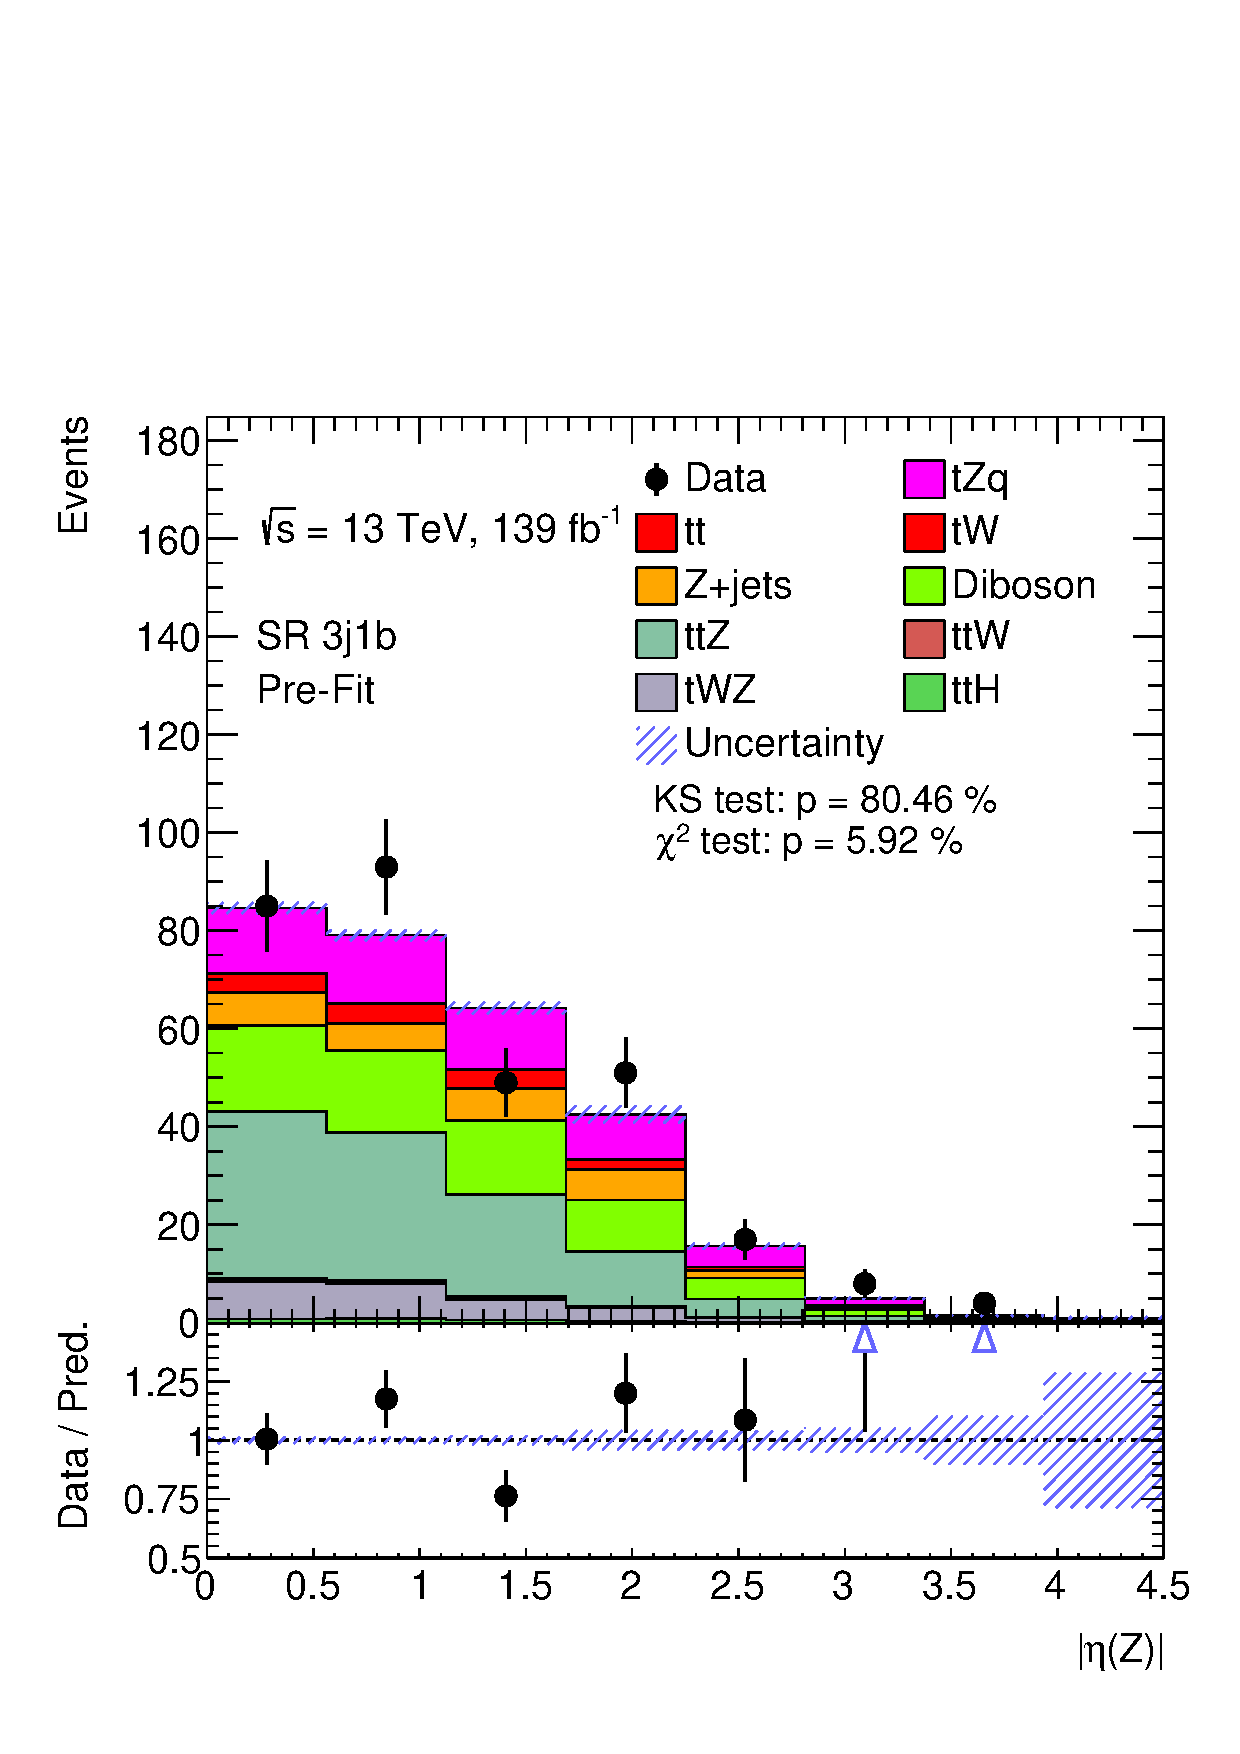
\includegraphics[width=\linewidth]{ubonn-thesis/Chapters/Chapters_05/Figure/SR/SR_3j1b_Z_eta.pdf} 
  \end{subfigure}
  \begin{subfigure}[b]{0.33\linewidth}
    \centering
    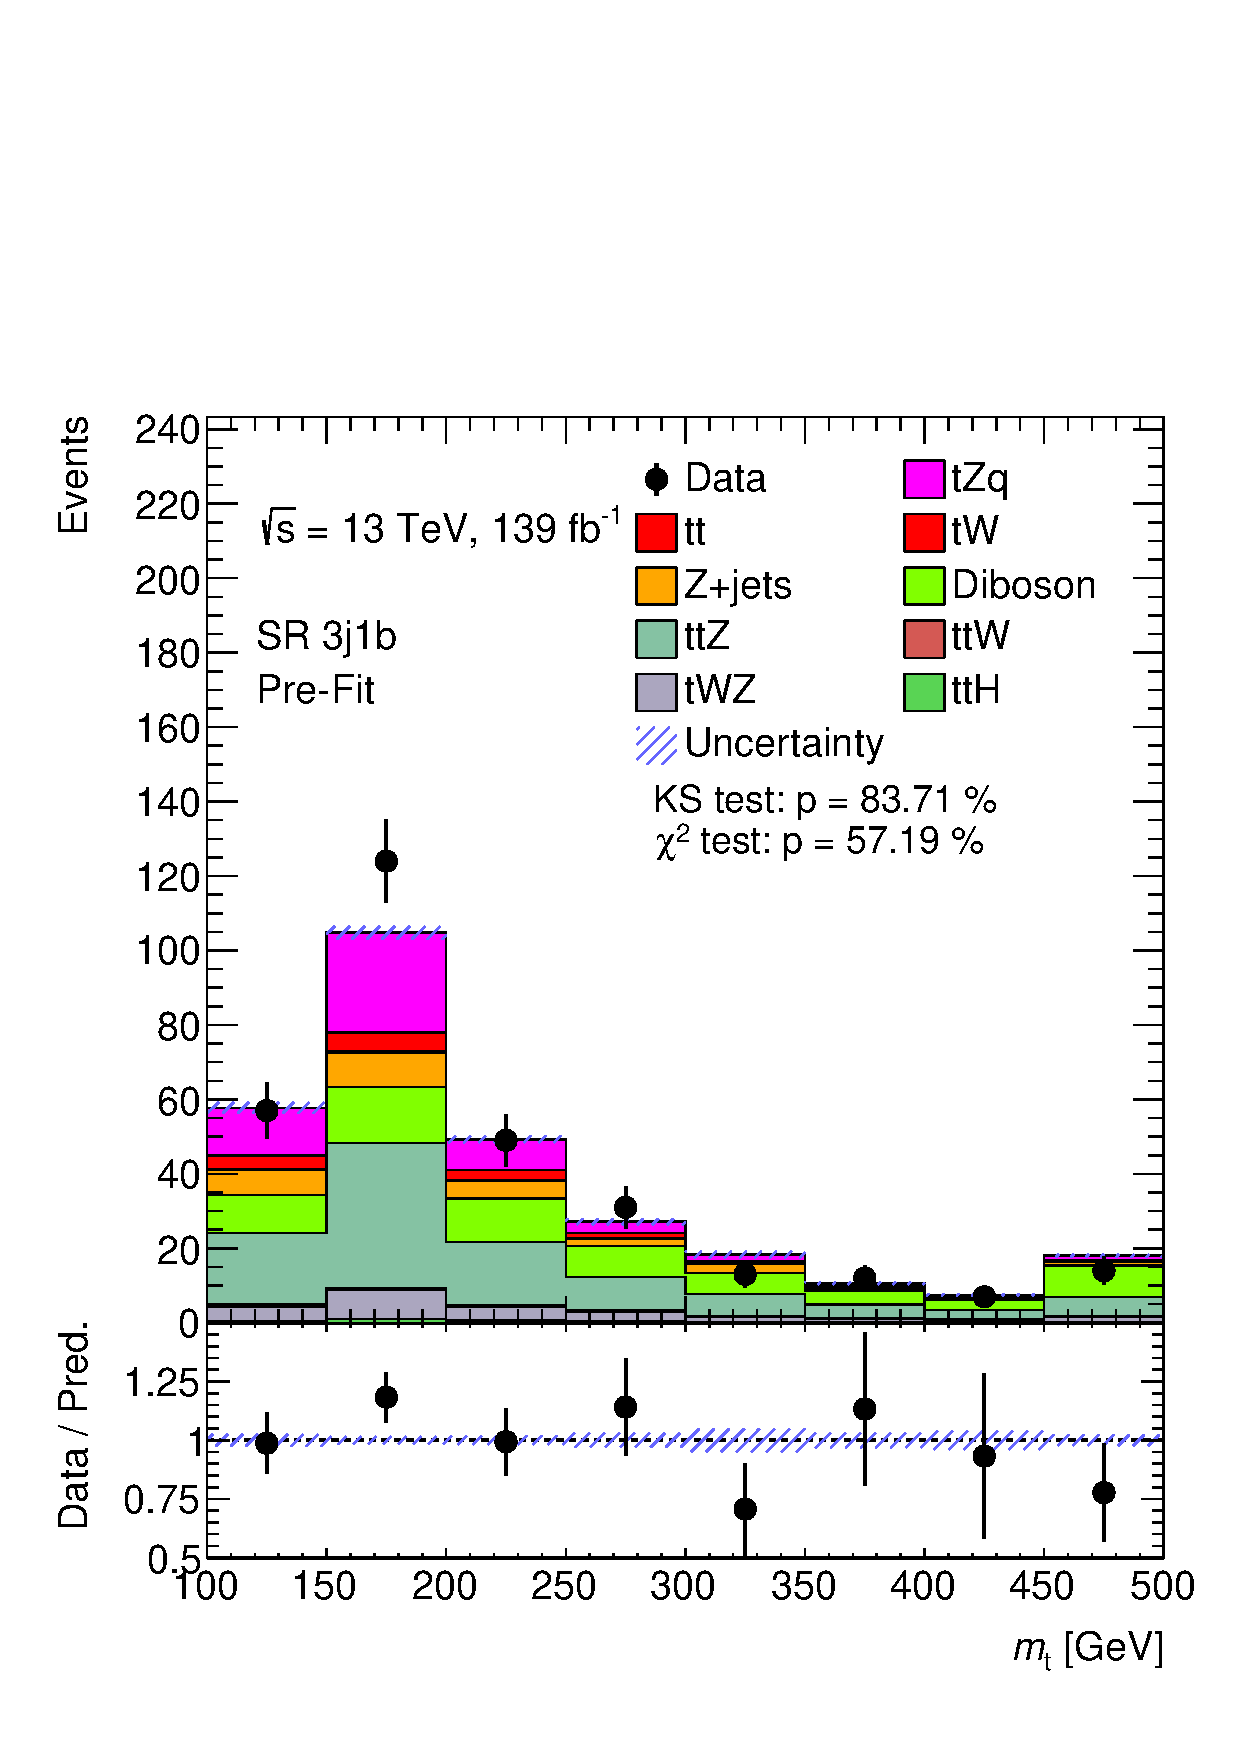
\includegraphics[width=\linewidth]{ubonn-thesis/Chapters/Chapters_05/Figure/SR/SR_3j1b_Top_mass.pdf} 
  \end{subfigure} 
  \caption{Comparison of data and MC predictions for reconstructed event related quantities for events in the SR 2j1b and SR 3j1b. The uncertainty shown is the statistical uncertainty}
  \label{fig:signal} 
\end{figure}






\section{Control regions (CRs)}
\label{sec:CR}

In order to ensure proper modeling of each relevant background, a series of control regions as listed in table \ref{tab:final_selection} are defined. These regions are constructed such that they are enriched in three of the main sources of backgrounds: diboson, $t\Bar{t}Z$, and $t\Bar{t}$ production. There are two CRs for each background, and one corresponding to each signal region.

\subsection{Diboson CRs plots and yields}
\label{subsec:diboson_plot_yield}

To define regions of phase space enriched in diboson production, the b-jet is vetoed. This leads to events such as WZ to dominate while effectively removing the events containing the top quark. This region also has significant contamination from Z+jets events. 

\begin{table}[!h]
    \begin{minipage}{.49\textwidth}
      \centering
      \begin{adjustbox}{width=\textwidth}
       \begin{tabular}{@{} *3l @{}}
 \toprule
 Process & Number of events & Number of raw events  \\ [0.5ex] 
 \hline\hline
  tZq   &  61.94 \pm 0.57 & 40215200 \\ 
  tt   &  14.58 \pm 0.73 & 64357  \\ 
  tW   & 0.49 \pm 0.75   &  556 \\ 
  Z+jets   & 152.32 \pm 18.75 & 624666  \\ 
  Diboson   & 2625.59 \pm 5.02  & 146163000  \\ 
  ttZ   & 48.59 \pm 4.79 &  4766730 \\ 
  ttW   & 1.85 \pm 0.11 & 98134 \\ 
  tWZ   & 17.10 \pm 0.54 & 422977 \\ 
  ttH   & 1.14 \pm 0.03   & 323175 \\ 
\hline 
  Total expected  & 2923.59 \pm 17.11  & 192679000 \\ 
\hline 
  Data   & 3116   & 3116 \\  
 \bottomrule
 \end{tabular} 
 \end{adjustbox}
    \end{minipage}%
    \hfill
    %\hspace{-1.5cm}
    \begin{minipage}{.49\textwidth}
      \centering
      \vspace*{0.5cm}
      \begin{adjustbox}{width=\textwidth}
        \begin{tabular}{@{} *3l @{}}
 \toprule
 Process & Number of events & Number of raw events  \\ [0.5ex] 
 \hline\hline
   tZq   &  25.58 \pm 0.42 & 21530100 \\ 
  tt   & 5.59 \pm 0.46 & 24603  \\ 
  tW   & 0.60 \pm 0.42 & 695 \\ 
  Z+jets & 52.53 \pm 5.89  & 244640  \\ 
  Diboson  & 973.45 \pm 2.35 & 60037700 \\ 
  ttZ   & 47.15 \pm 1.42 & 6095710 \\ 
  ttW   & 0.88 \pm 0.09 & 51847  \\ 
  tWZ   & 13.13 \pm 0.51  & 375439 \\ 
  ttH   & 1.07 \pm 0.03 & 268270 \\ 
\hline 
  Total expected  & 1119.97 \pm 6.51 & 88629000 \\ 
\hline 
  Data    & 1083 & 1083 \\ 
 \bottomrule
 \end{tabular} 
 \end{adjustbox}
    \end{minipage} 
    \caption{Numbers of expected events in the CR 2j0b (Left) and CR 3j0b (Right) broken down by process. The uncertainty shown contains only the statistical component.}
 \label{tab:yield_diboson}
\end{table}


\begin{figure}[h!] 
  \begin{subfigure}[b]{0.33\linewidth}
    \centering
    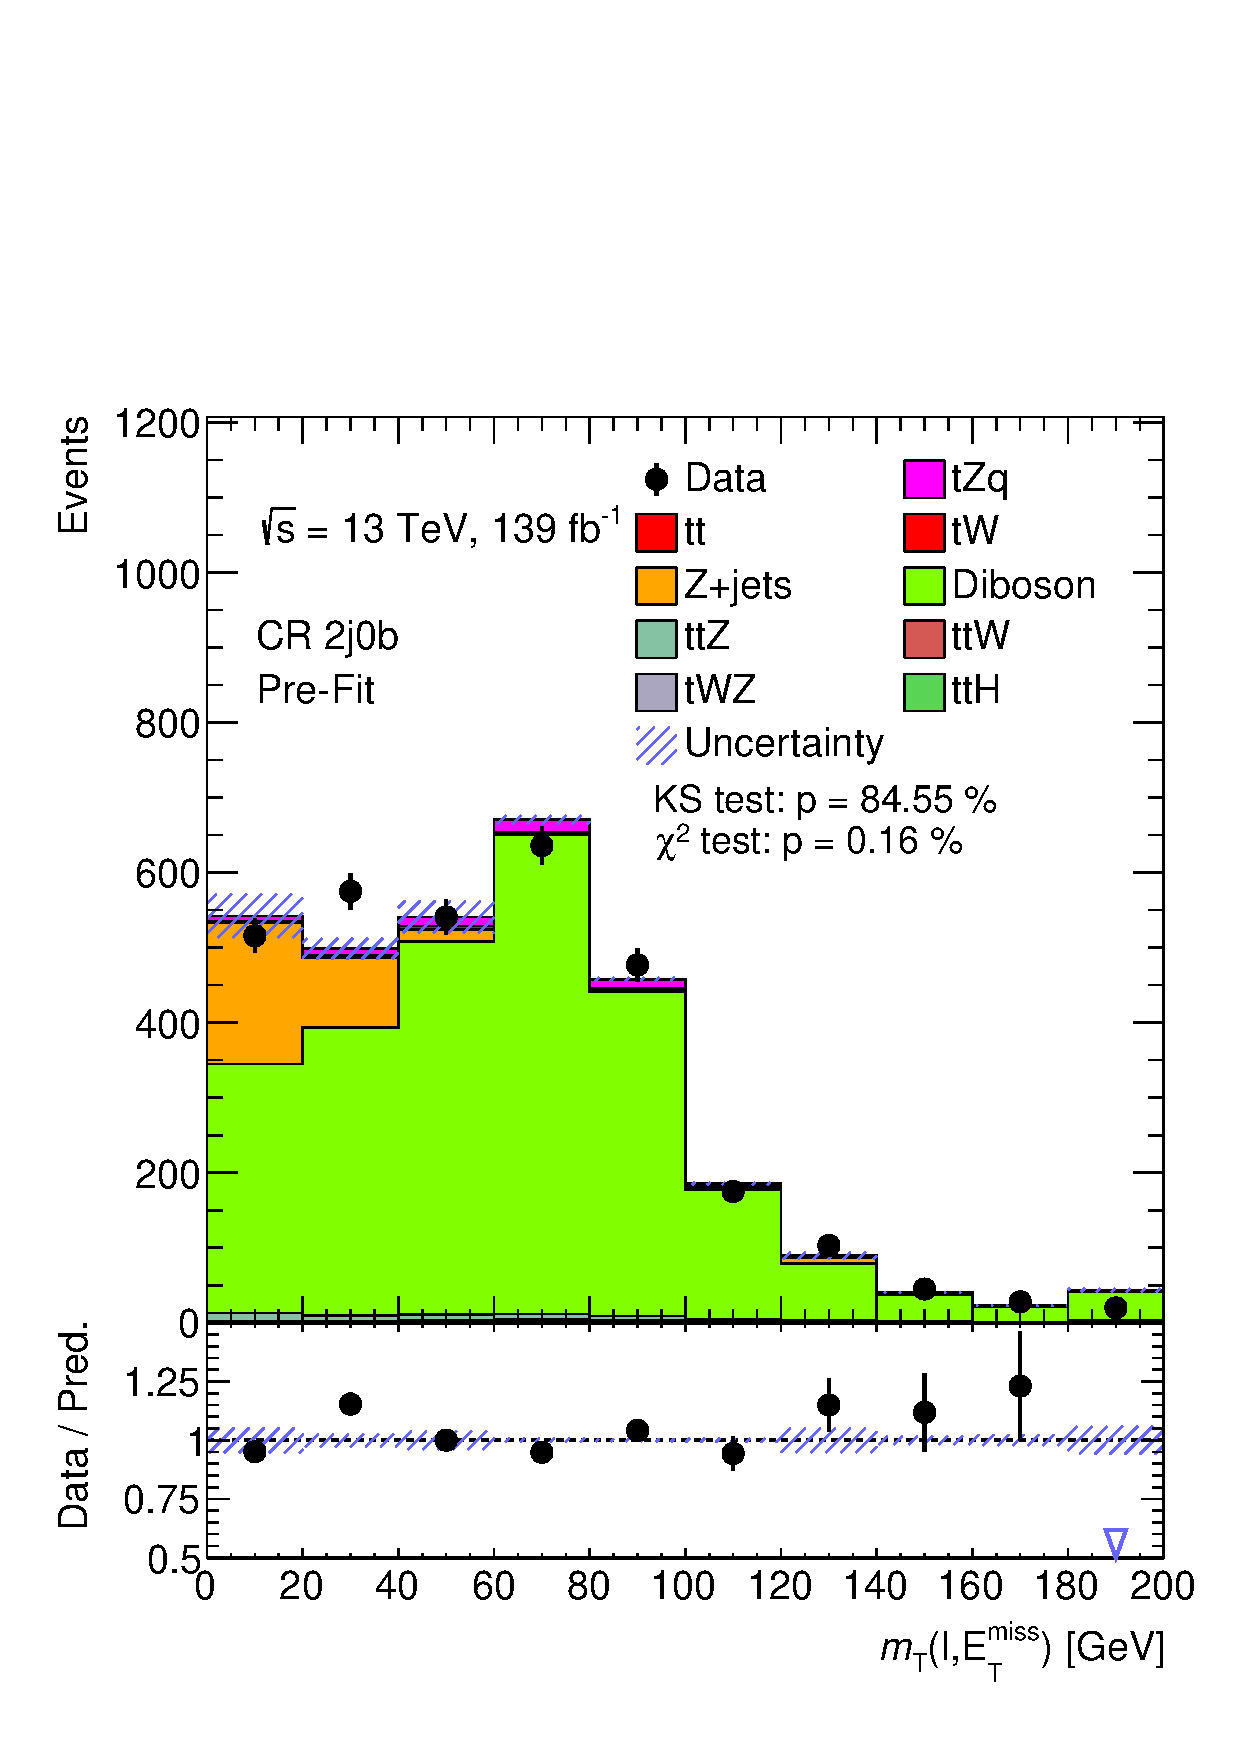
\includegraphics[width=\linewidth]{ubonn-thesis/Chapters/Chapters_05/Figure/CR_VV/CR_2j0b_mtW.pdf} 
  \end{subfigure} 
  \begin{subfigure}[b]{0.33\linewidth}
    \centering
    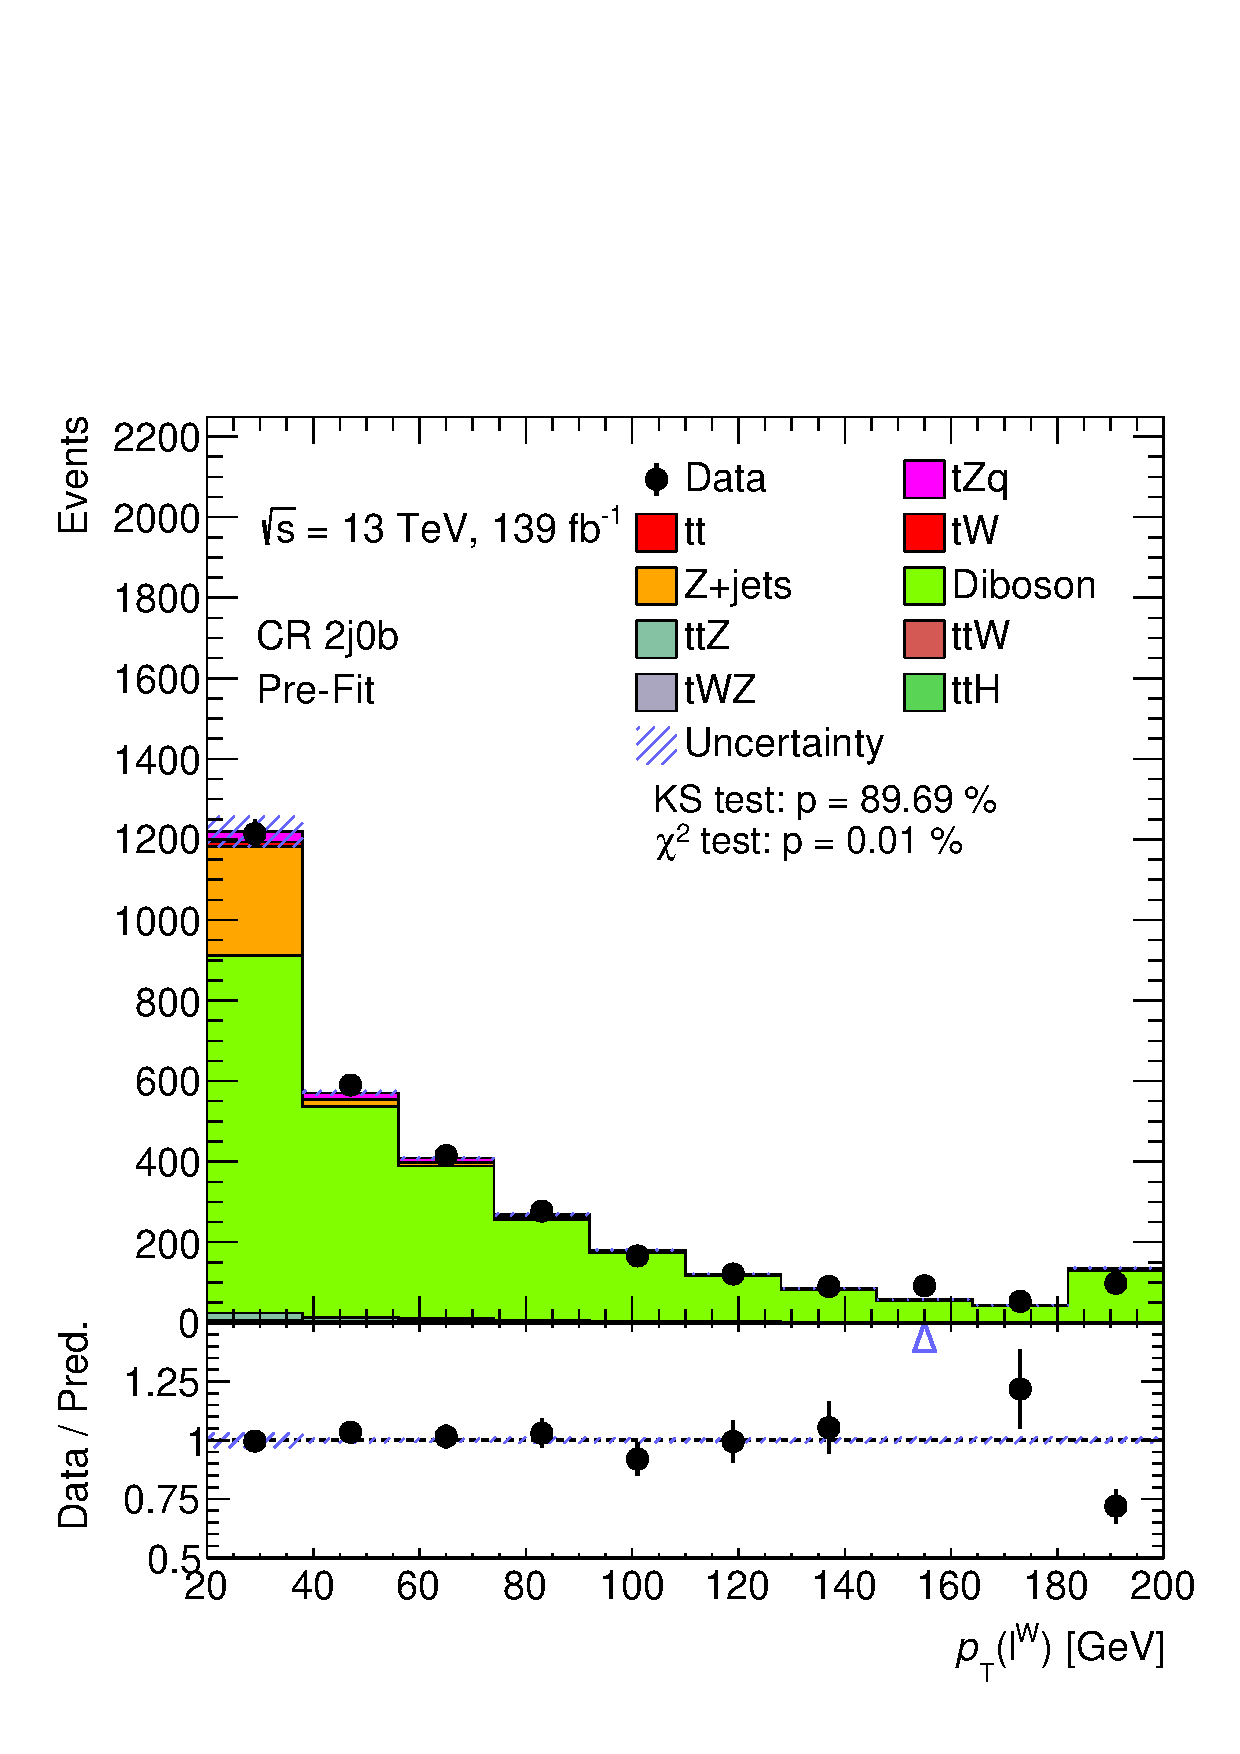
\includegraphics[width=\linewidth]{ubonn-thesis/Chapters/Chapters_05/Figure/CR_VV/CR_2j0b_lepW_pt.pdf} 
  \end{subfigure}%%
  \begin{subfigure}[b]{0.33\linewidth}
    \centering
    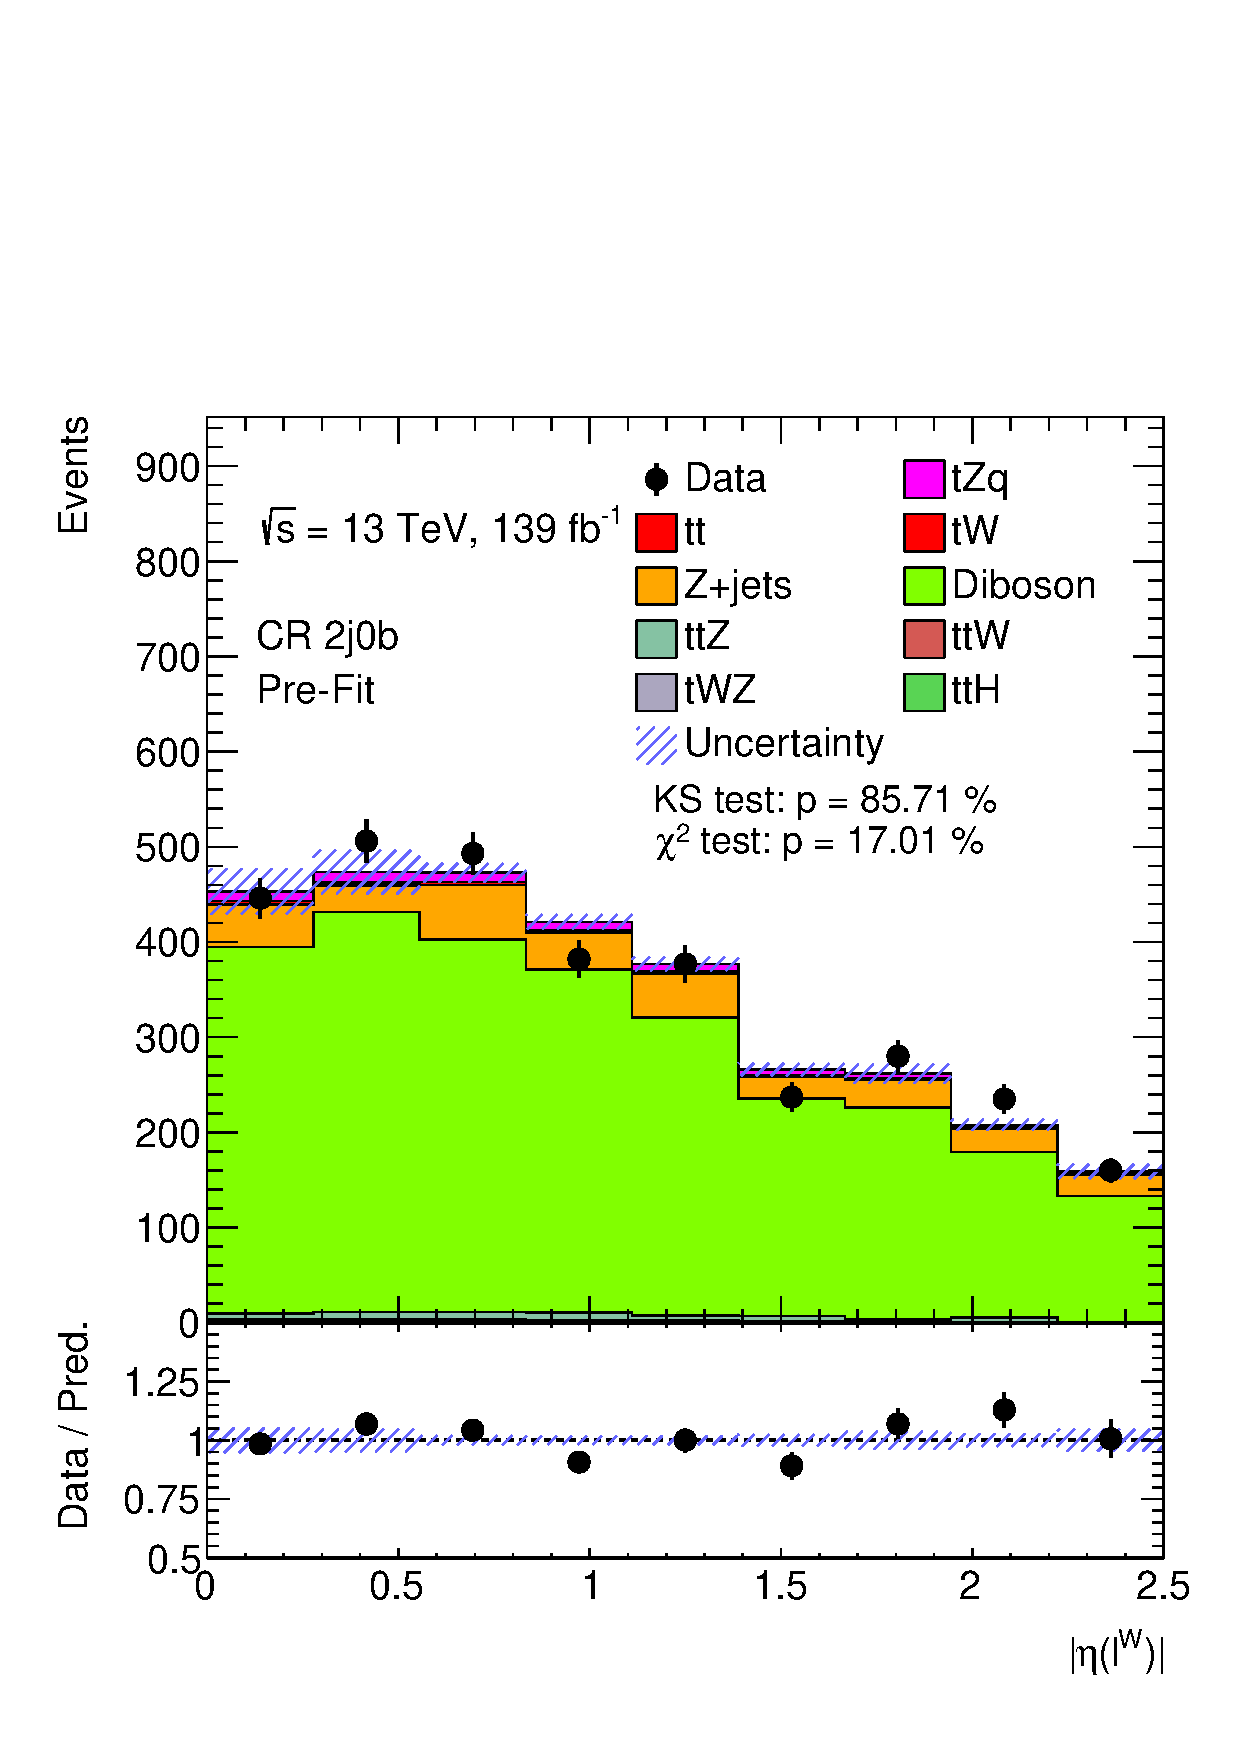
\includegraphics[width=\linewidth]{ubonn-thesis/Chapters/Chapters_05/Figure/CR_VV/CR_2j0b_lepW_eta.pdf} 
  \end{subfigure} 
  \newline
  \begin{subfigure}[b]{0.33\linewidth}
    \centering
    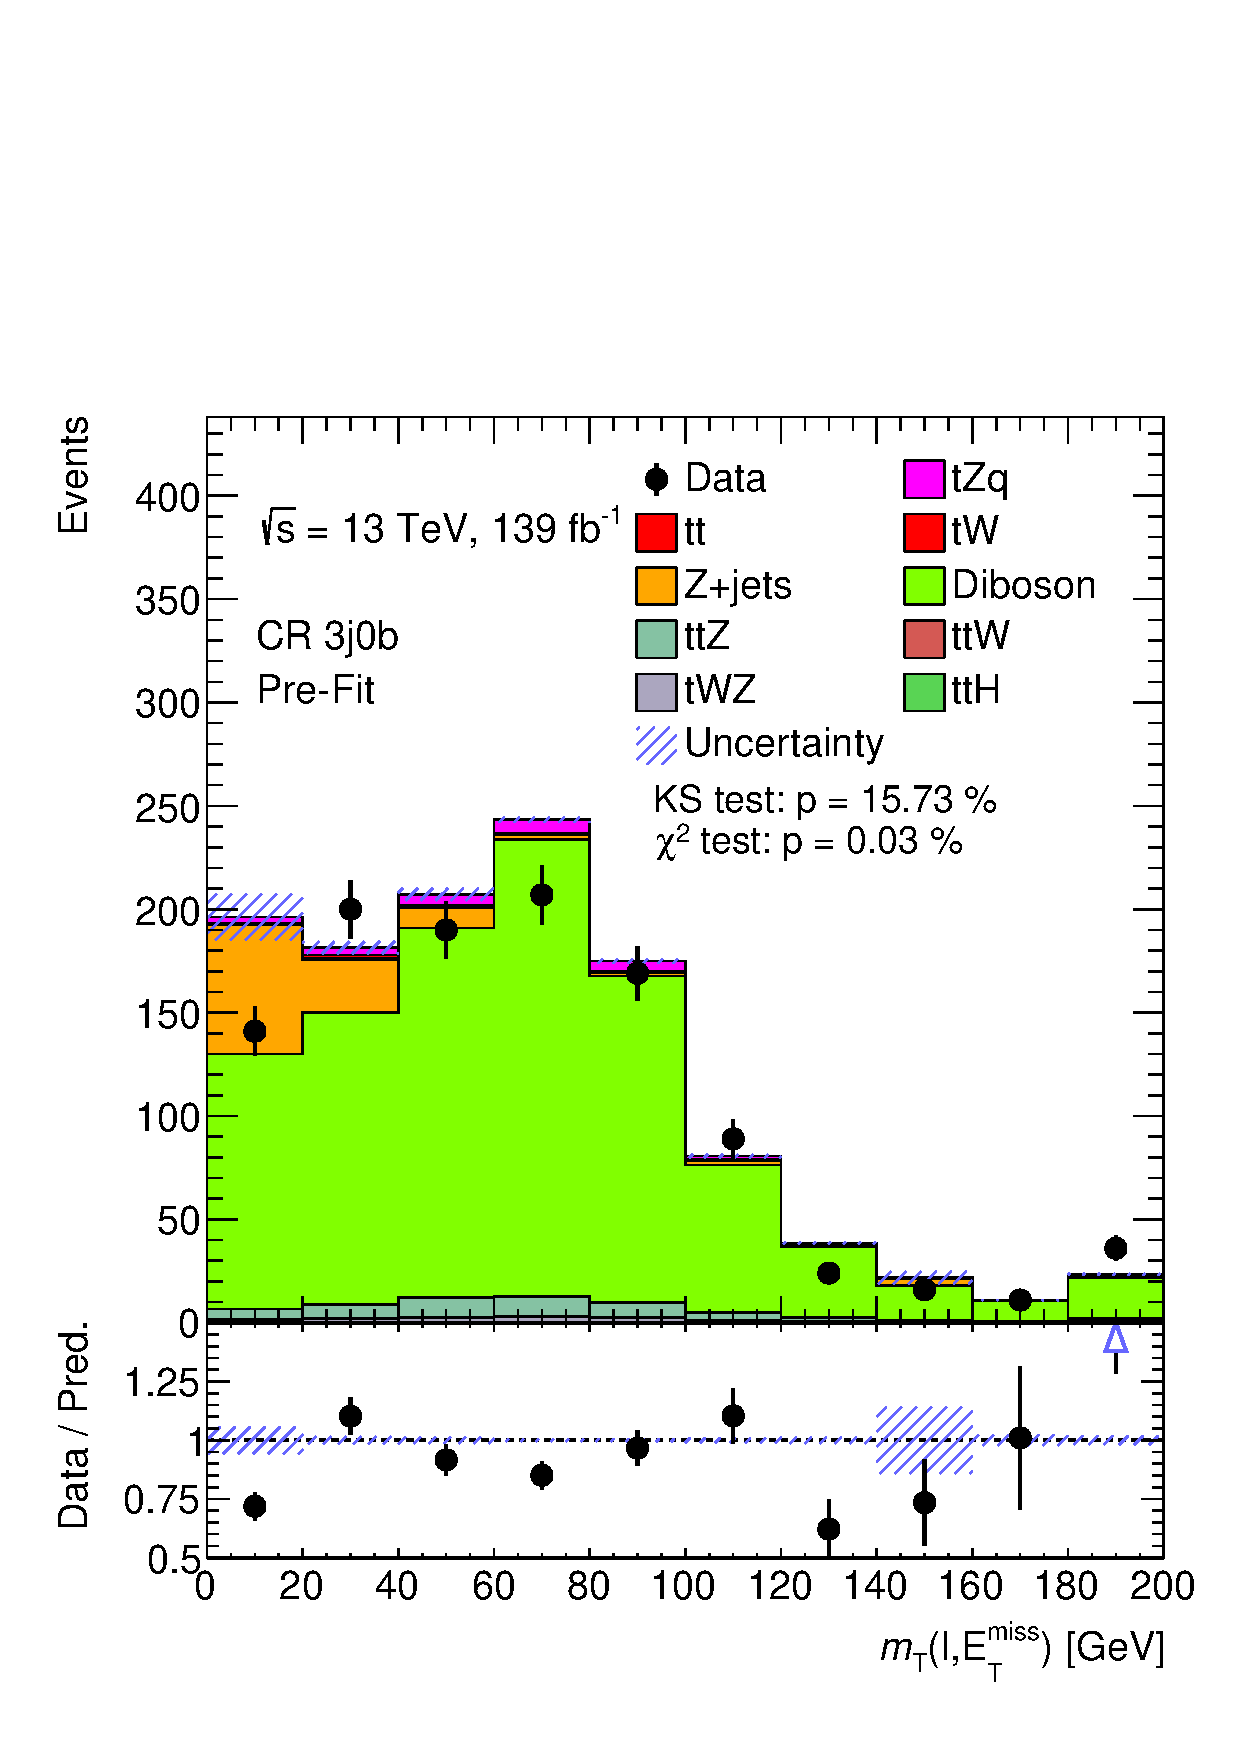
\includegraphics[width=\linewidth]{ubonn-thesis/Chapters/Chapters_05/Figure/CR_VV/CR_3j0b_mtW.pdf} 
  \end{subfigure} 
  \begin{subfigure}[b]{0.33\linewidth}
    \centering
    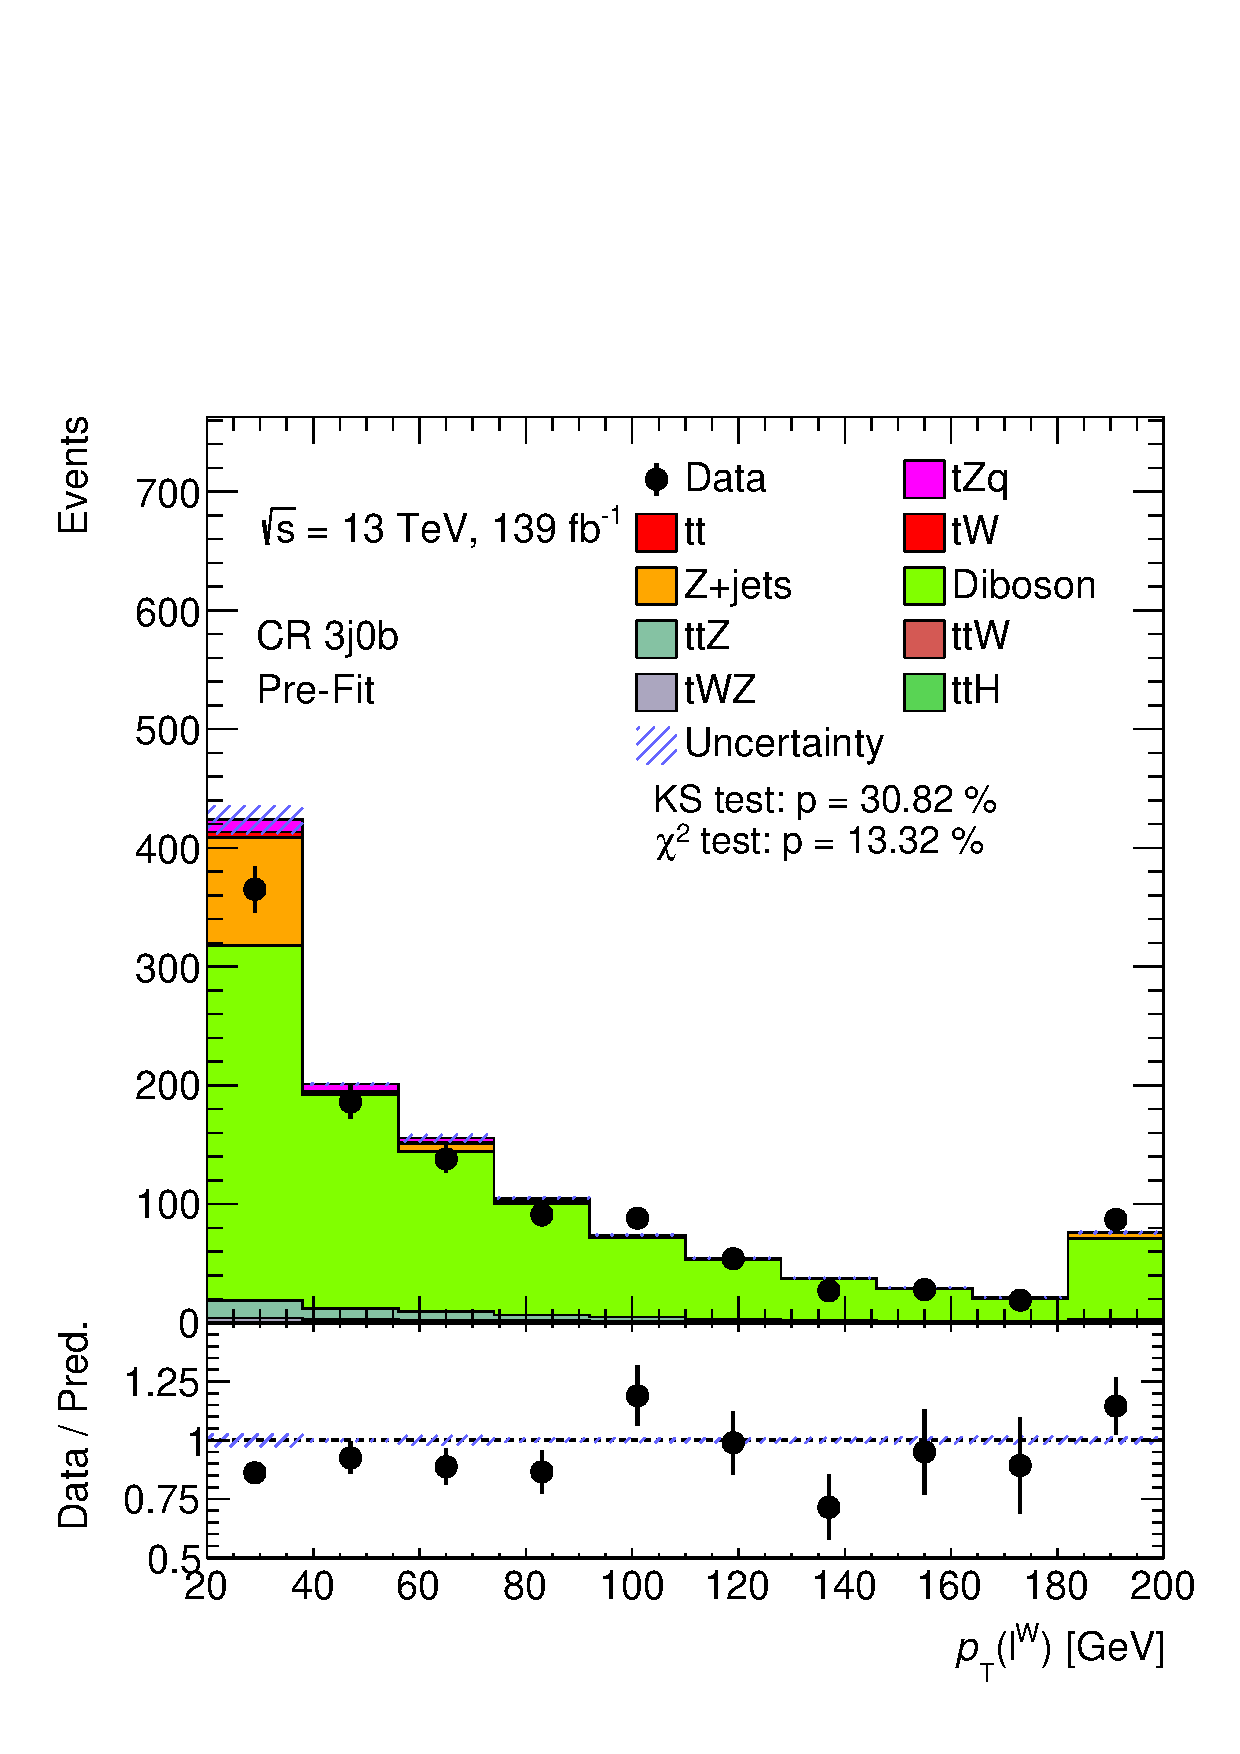
\includegraphics[width=\linewidth]{ubonn-thesis/Chapters/Chapters_05/Figure/CR_VV/CR_3j0b_lepW_pt.pdf} 
  \end{subfigure}%%
  \begin{subfigure}[b]{0.33\linewidth}
    \centering
    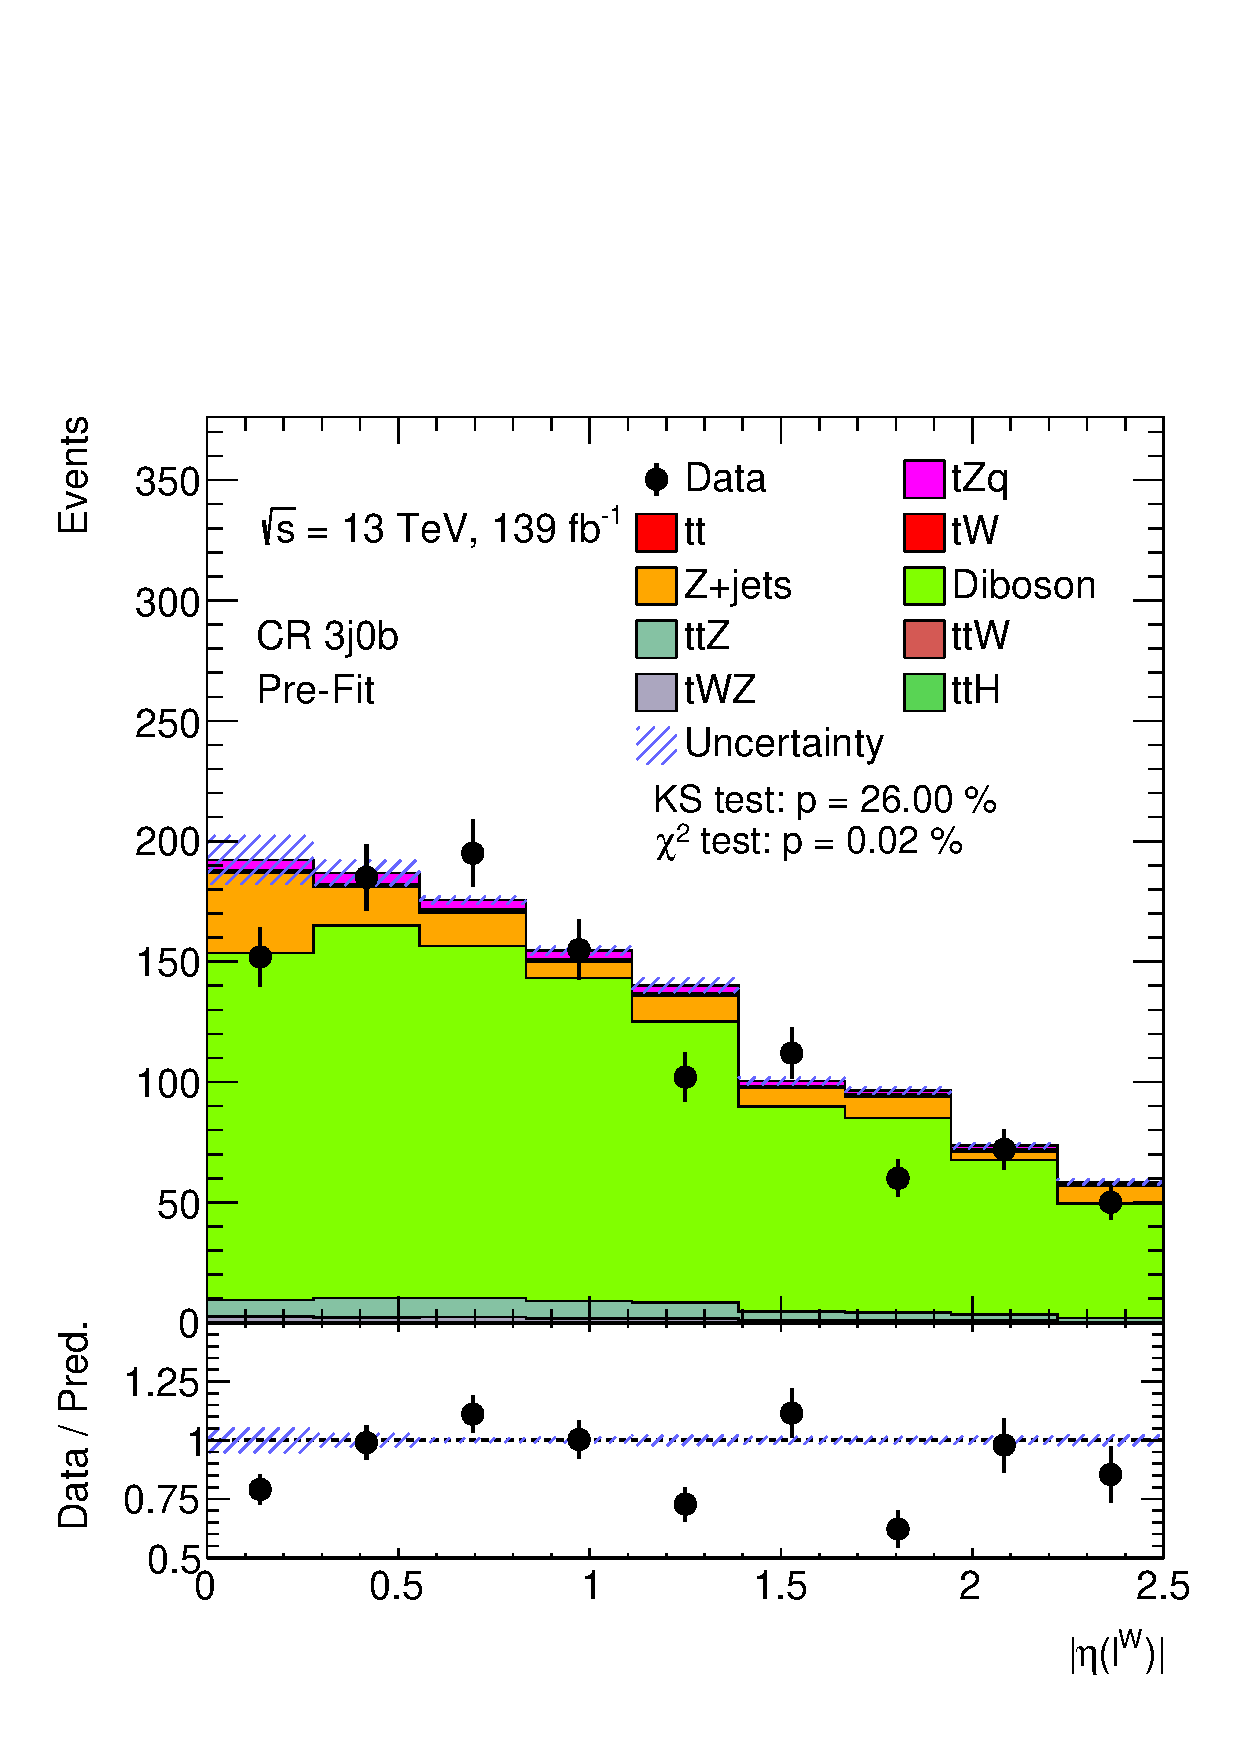
\includegraphics[width=\linewidth]{ubonn-thesis/Chapters/Chapters_05/Figure/CR_VV/CR_3j0b_lepW_eta.pdf} 
  \end{subfigure} 
  \caption{Comparison of data and MC predictions for reconstructed event related quantities for events in the CR 2j0b and CR 3j0b. }
  \label{fig:CRdibson}
  \end{figure}


 
The two diboson control regions are listed in table \ref{tab:final_selection}. The events yields in diboson CRs after the full section are shown in table \ref{tab:yield_diboson}. Some of the reconstructed variables in this control regions are shown in figure \ref{fig:CRdibson}.
The large number of observed events in this control region helps to provide a significant constraint on the overall rate of diboson events.  


\subsection{$t\Bar{t}Z$ CRs plots and yield}
\label{subsec:ttZ_plot_yield}


To define regions of phase space enriched in $t\Bar{t}Z$ production, an additional b-jet is required to enhance events with a second top quark. This region also contains significant amount of signal events. 

\vspace*{-0.4cm}
\begin{table}[!h]
    \begin{minipage}{.49\textwidth}
      \centering
      \begin{adjustbox}{width=\textwidth}
       \begin{tabular}{@{} *3l @{}}
 \toprule
 Process & Number of events & Number of raw events  \\ [0.5ex] 
 \hline\hline
  tZq   & 15.78 \pm 0.23 & 6584710\\ 
  tt   & 2.31 \pm 0.30 & 11120  \\ 
  tW   & 0.08 \pm 0.43   & 139 \\ 
  Z+jets   &  1.10 \pm 0.19 & 8062 \\ 
  Diboson   & 5.48 \pm 0.16  & 381555 \\ 
  ttZ   & 48.94 \pm 0.45 & 5681490 \\ 
  ttW   &  1.69 \pm 0.12 & 105501  \\ 
  tWZ   & 3.91 \pm 0.26 & 100775 \\ 
  ttH   & 1.59 \pm 0.04   & 488446 \\ 
\hline 
  Total expected  & 80.88 \pm 0.70 & 13361800  \\ 
\hline 
  Data   & 118  & 118  \\ 
 \bottomrule
 \end{tabular} 
 \end{adjustbox}
    \end{minipage}%
    \hfill
    \begin{minipage}{.49\textwidth}
      \centering
      \vspace*{0.5cm}
      \begin{adjustbox}{width=\textwidth}
        \begin{tabular}{@{} *3l @{}}
 \toprule
 Process & Number of events & Number of raw events  \\ [0.5ex] 
 \hline\hline
   tZq   & 10.43 \pm 0.20  & 5136470  \\ 
  tt   & 1.14 \pm 0.22 & 5699 \\ 
  tW   & 0.16 \pm 0.38 & 278  \\ 
  Z+jets & 0.56 \pm 0.13 & 4170 \\ 
  Diboson  & 3.38 \pm 0.12 & 230184 \\ 
  ttZ   & 53.35 \pm 0.51 & 7061060 \\ 
  ttW   & 0.76 \pm 0.07 & 42812  \\ 
  tWZ   & 4.76 \pm 0.29 & 120652  \\ 
  ttH   & 1.41 \pm 0.04  & 365153  \\ 
\hline 
  Total expected  & 75.94 \pm 0.68 & 12966500  \\ 
\hline 
  Data    & 77 & 77 \\  
 \bottomrule
 \end{tabular} 
 \end{adjustbox}
    \end{minipage} 
    \caption{Numbers of expected events in the CR 3j2b (Left) and CR 4j2b (Right) broken down by process. The uncertainty shown contains only the statistical component.}
    \label{tab:yield_ttZ}
\end{table}

\vspace*{-0.3cm}
\begin{figure}[h!] 
  \begin{subfigure}[b]{0.32\linewidth}
    \centering
    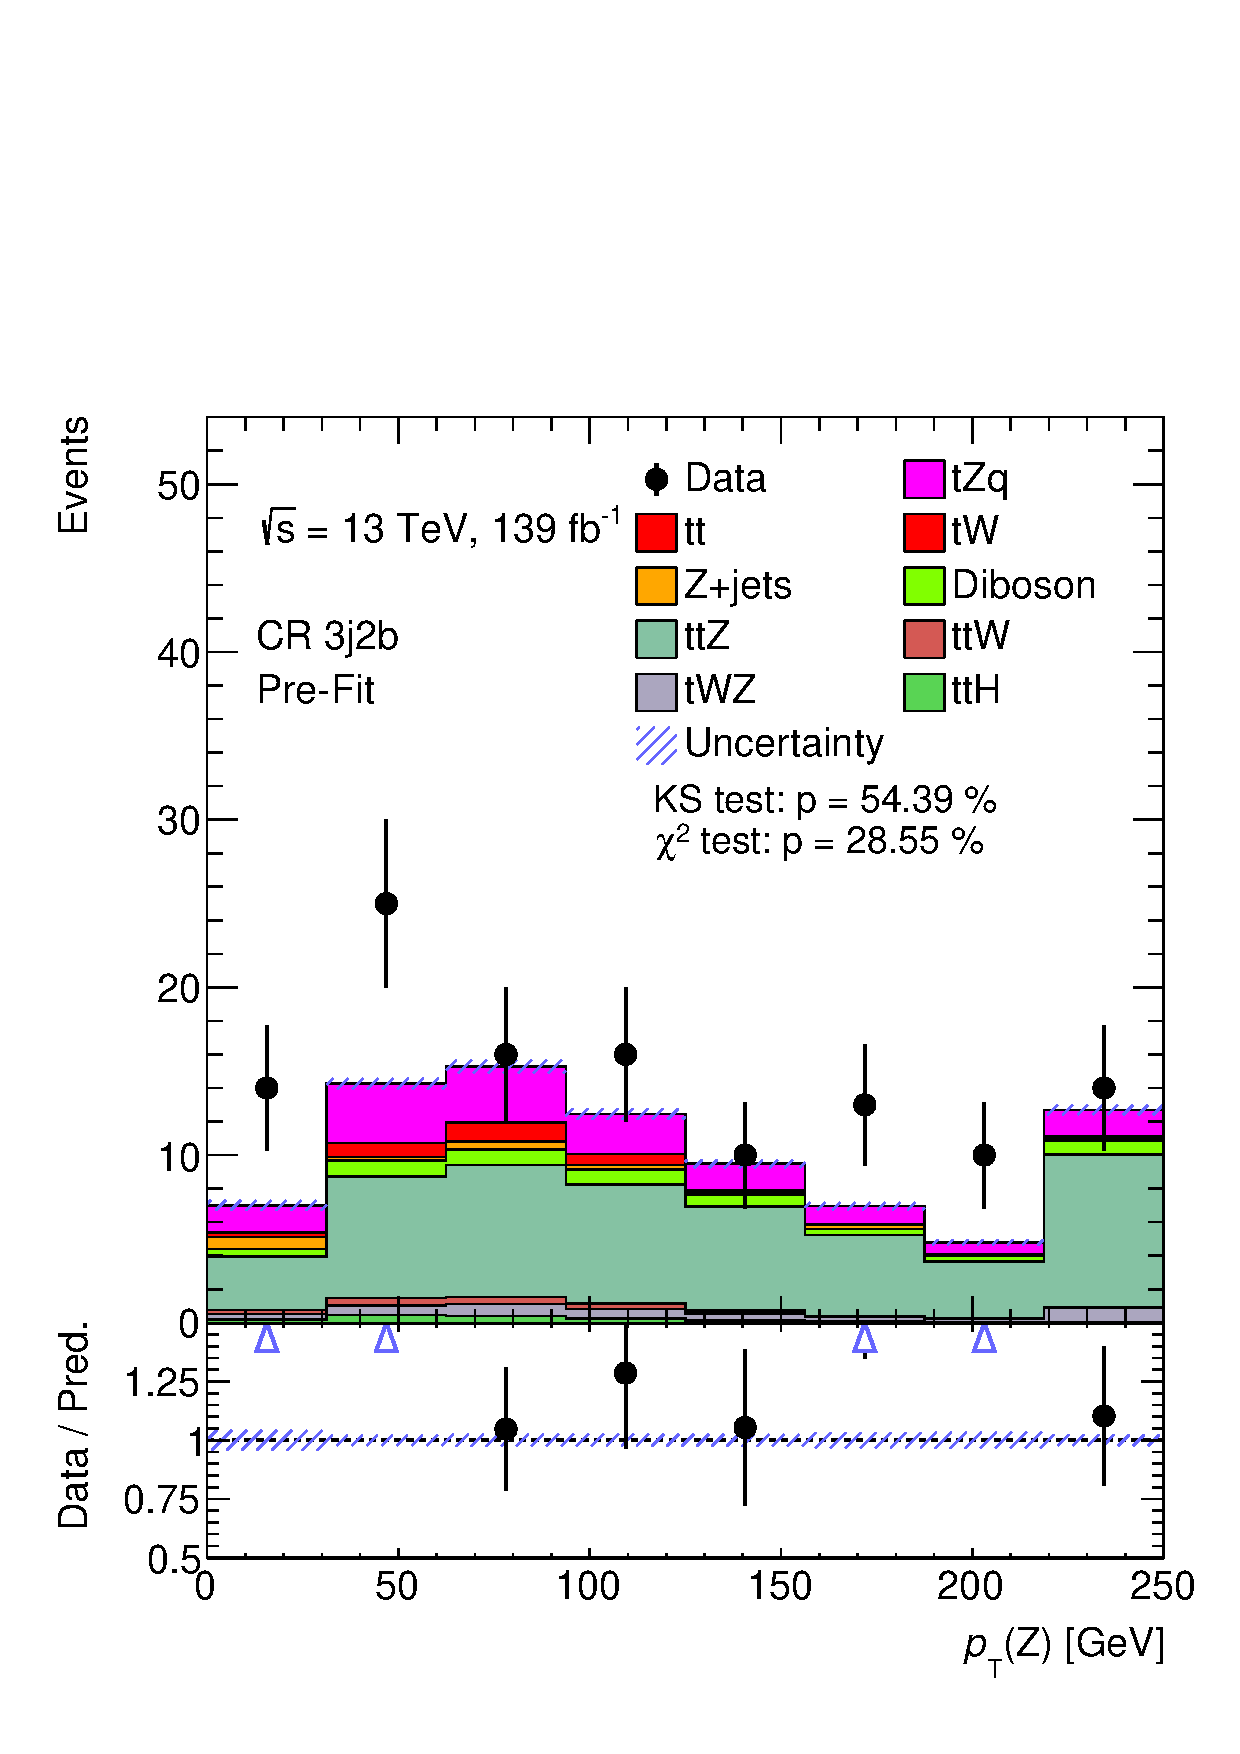
\includegraphics[width=\linewidth]{ubonn-thesis/Chapters/Chapters_05/Figure/CR_ttZ/CR_3j2b_Z_pt.pdf} 
  \end{subfigure}%% 
  \begin{subfigure}[b]{0.32\linewidth}
    \centering
    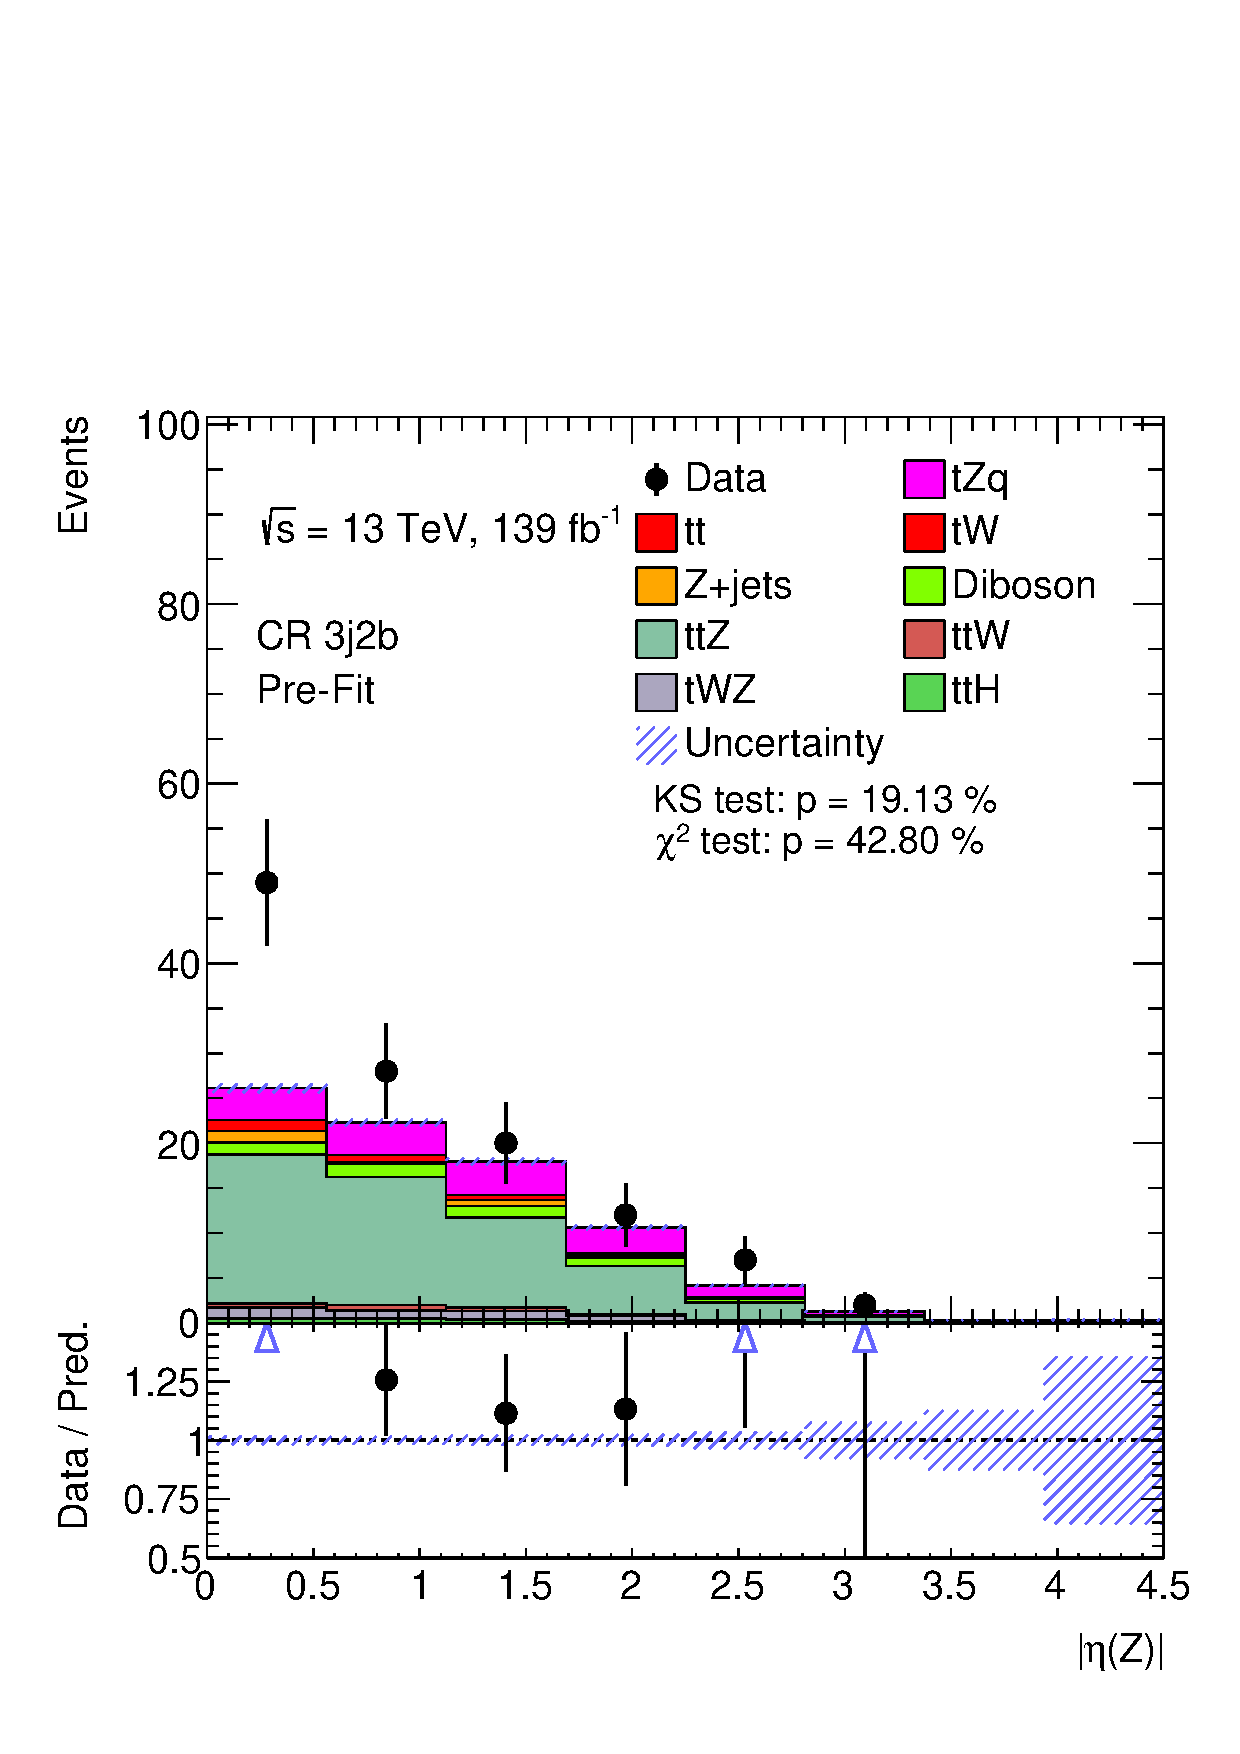
\includegraphics[width=\linewidth]{ubonn-thesis/Chapters/Chapters_05/Figure/CR_ttZ/CR_3j2b_Z_eta.pdf} 
  \end{subfigure} 
  \begin{subfigure}[b]{0.32\linewidth}
    \centering
    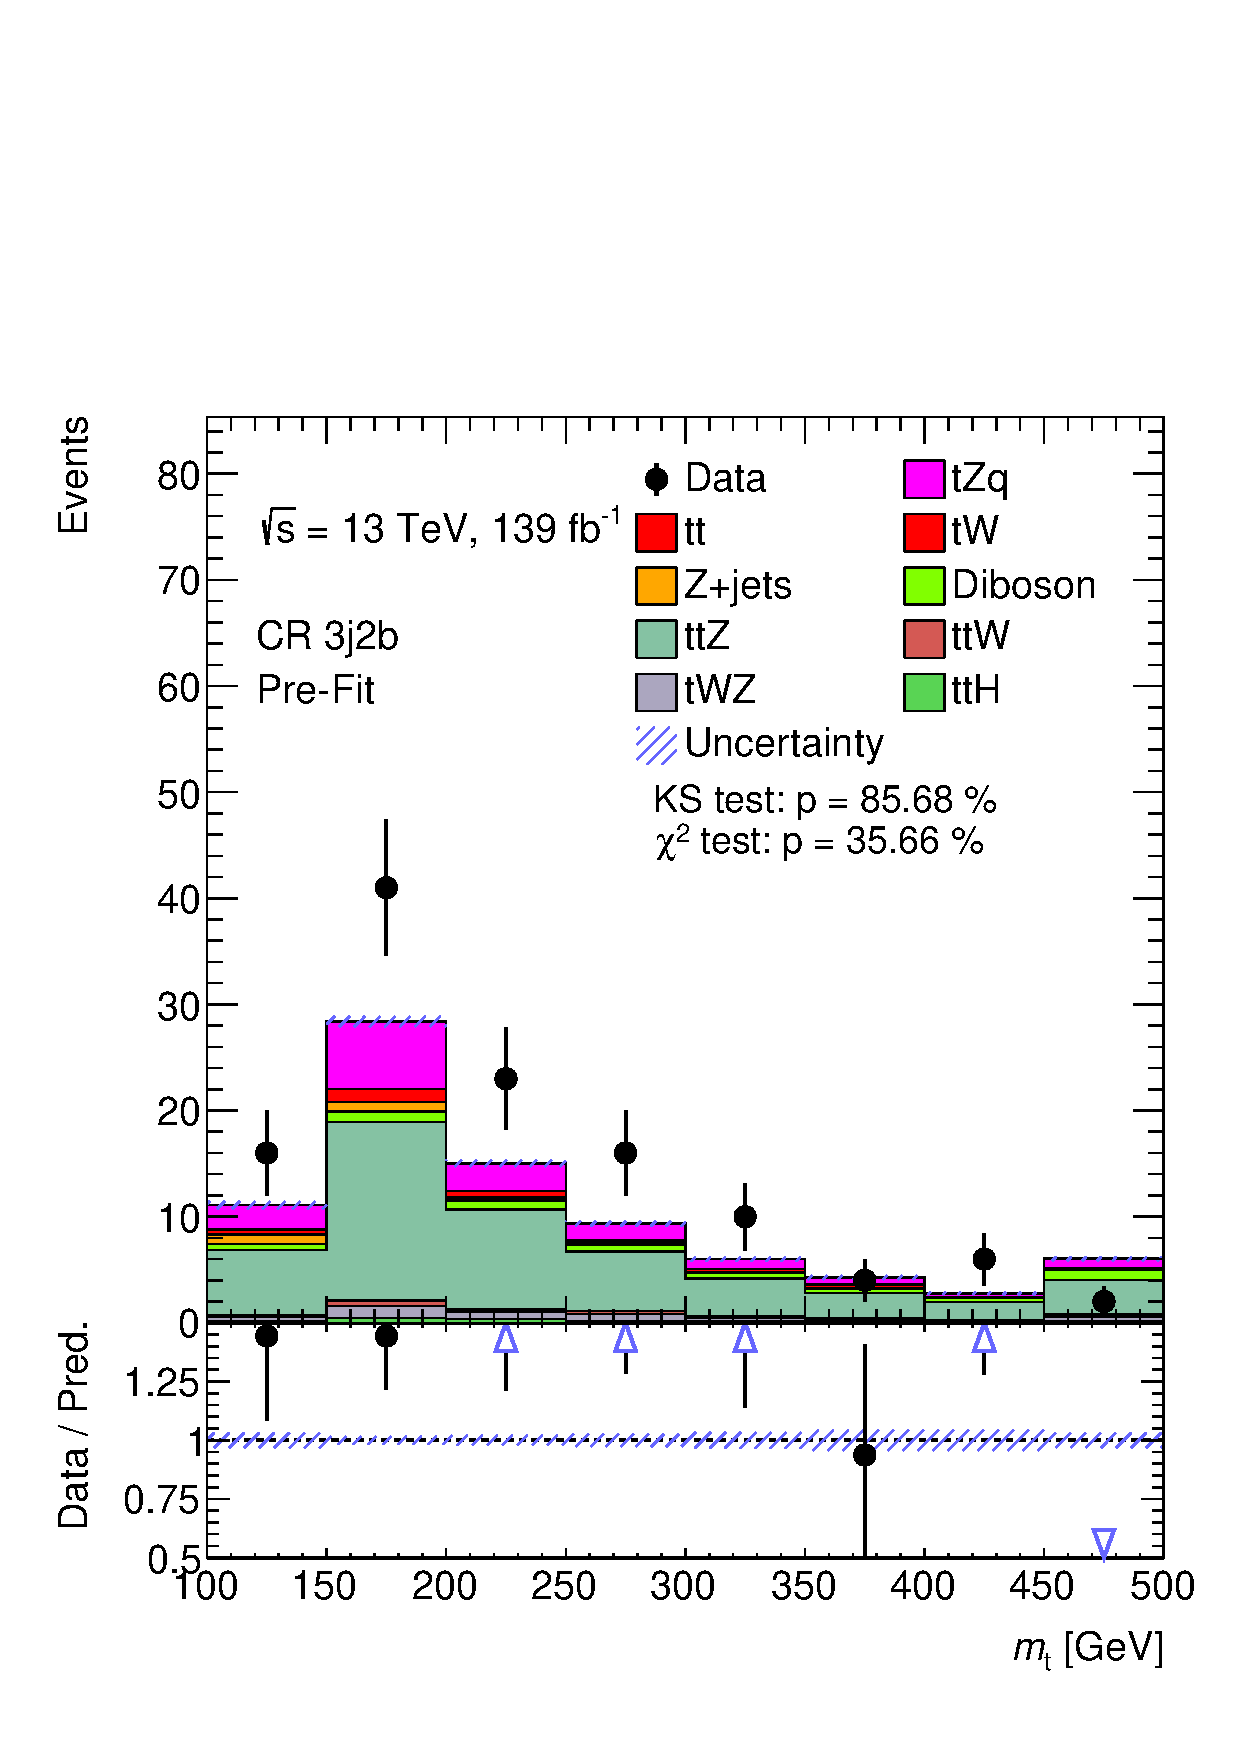
\includegraphics[width=\linewidth]{ubonn-thesis/Chapters/Chapters_05/Figure/CR_ttZ/CR_3j2b_Top_mass.pdf} 
  \end{subfigure}%%
  \newline
  \begin{subfigure}[b]{0.32\linewidth}
    \centering
    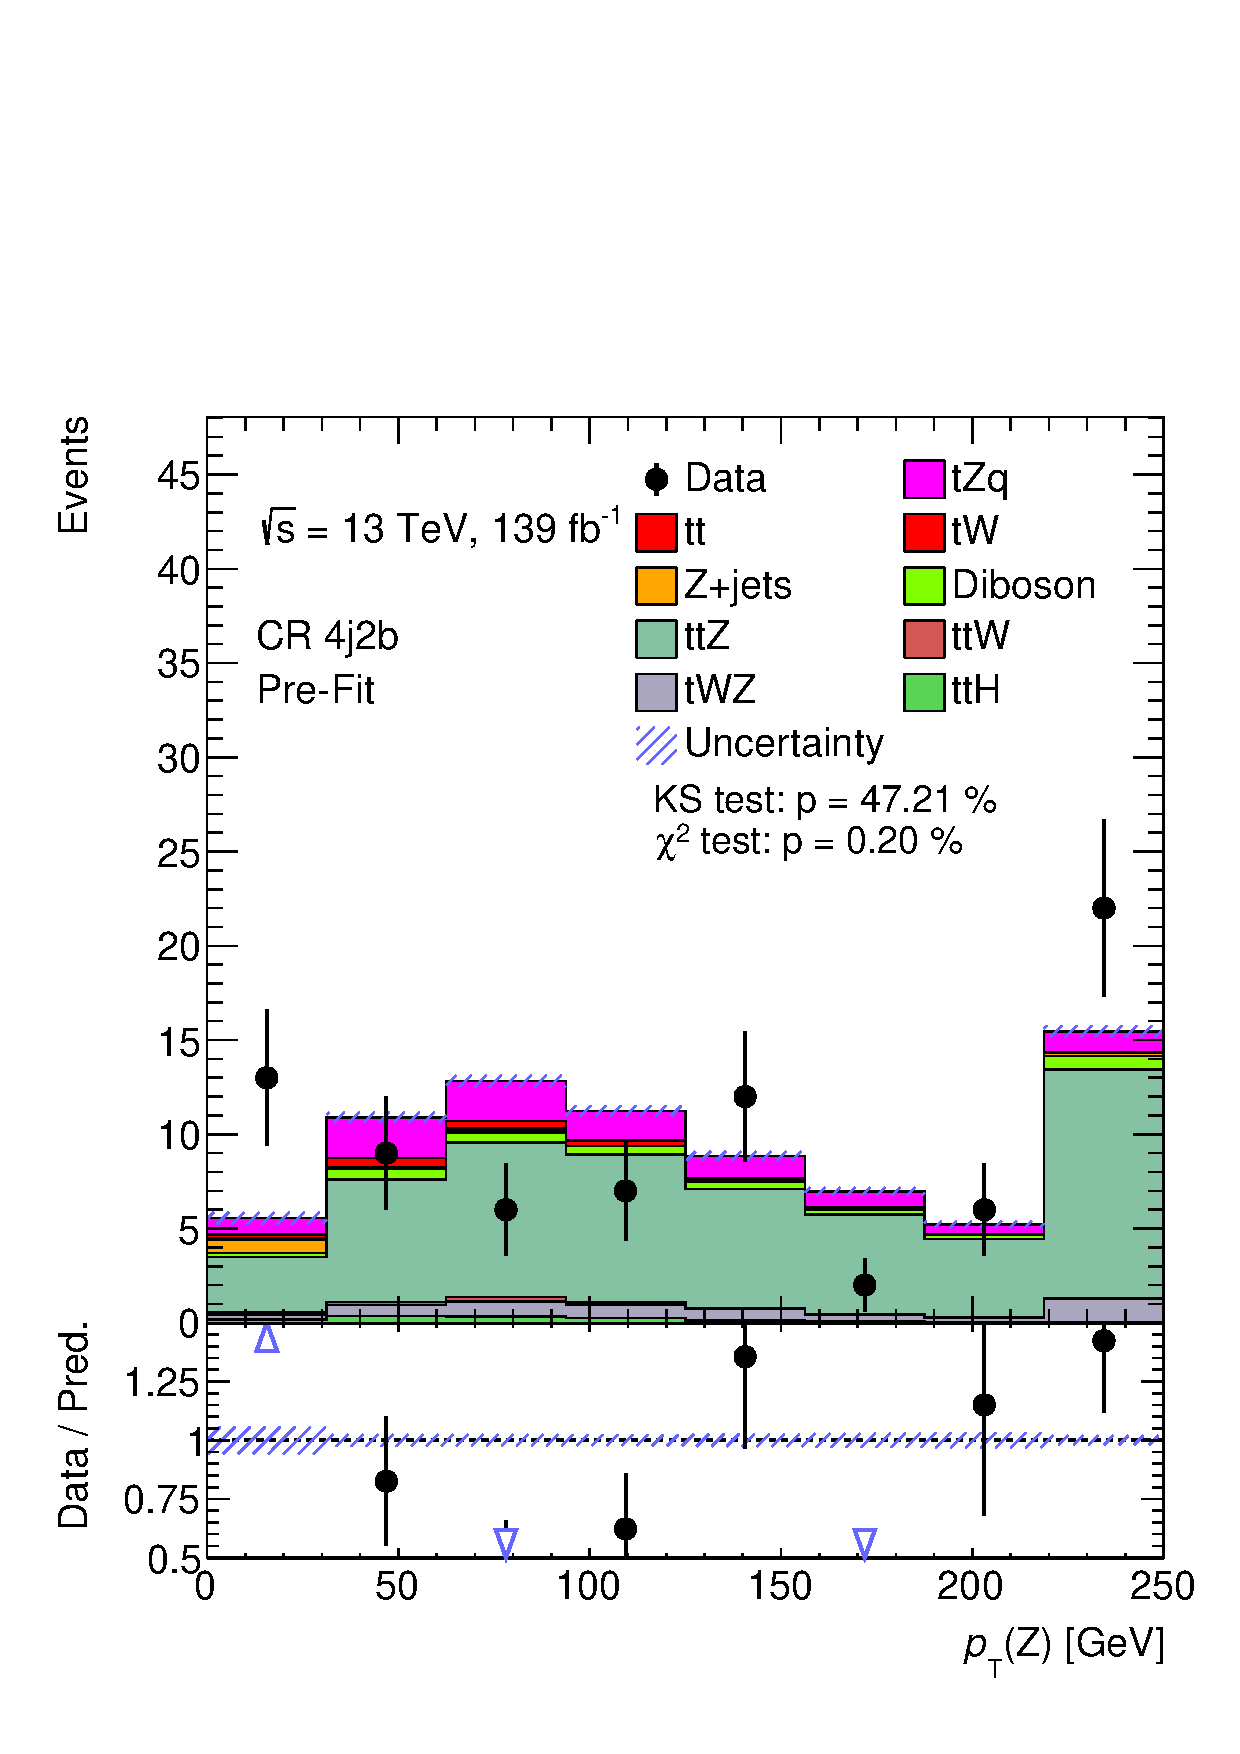
\includegraphics[width=\linewidth]{ubonn-thesis/Chapters/Chapters_05/Figure/CR_ttZ/CR_4j2b_Z_pt.pdf} 
  \end{subfigure} 
  \begin{subfigure}[b]{0.32\linewidth}
    \centering
    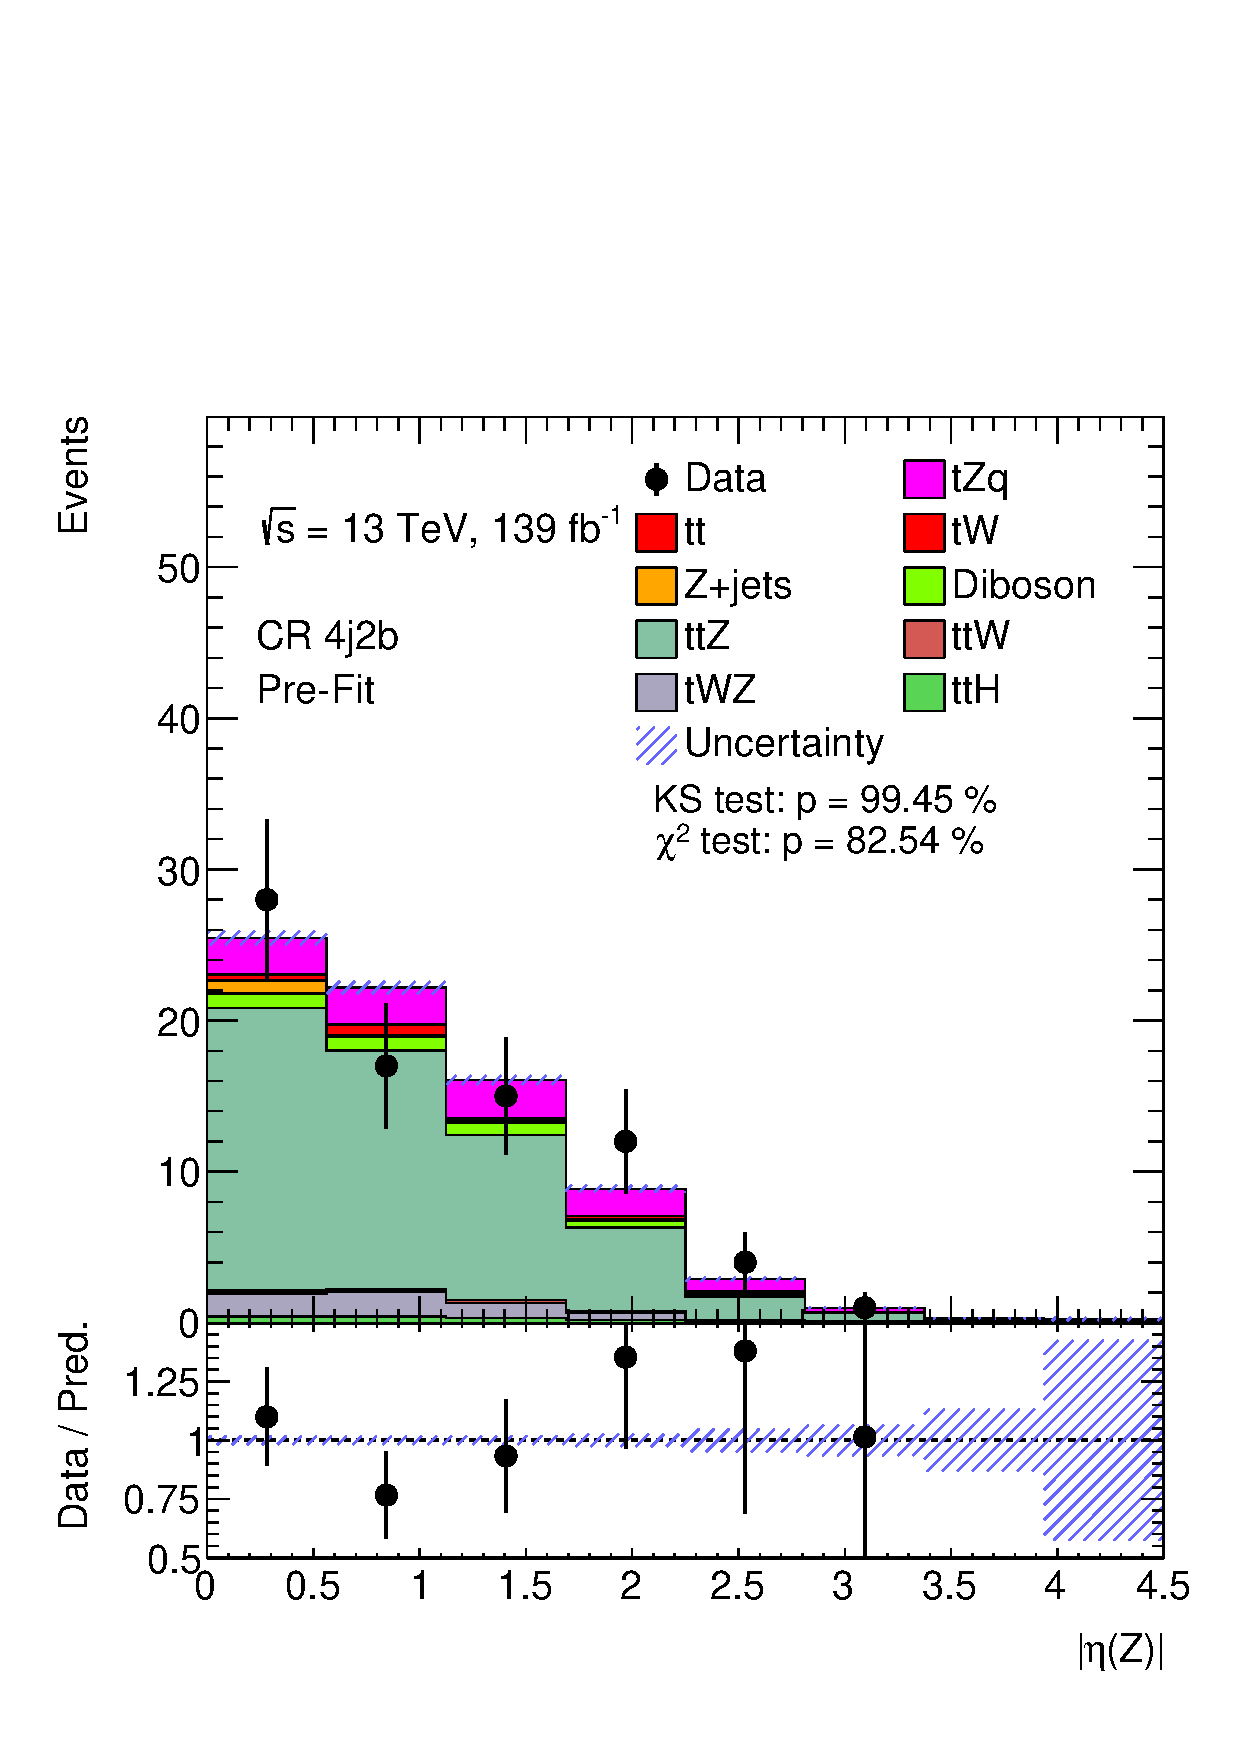
\includegraphics[width=\linewidth]{ubonn-thesis/Chapters/Chapters_05/Figure/CR_ttZ/CR_4j2b_Z_eta.pdf} 
  \end{subfigure}%% 
  \begin{subfigure}[b]{0.32\linewidth}
    \centering
    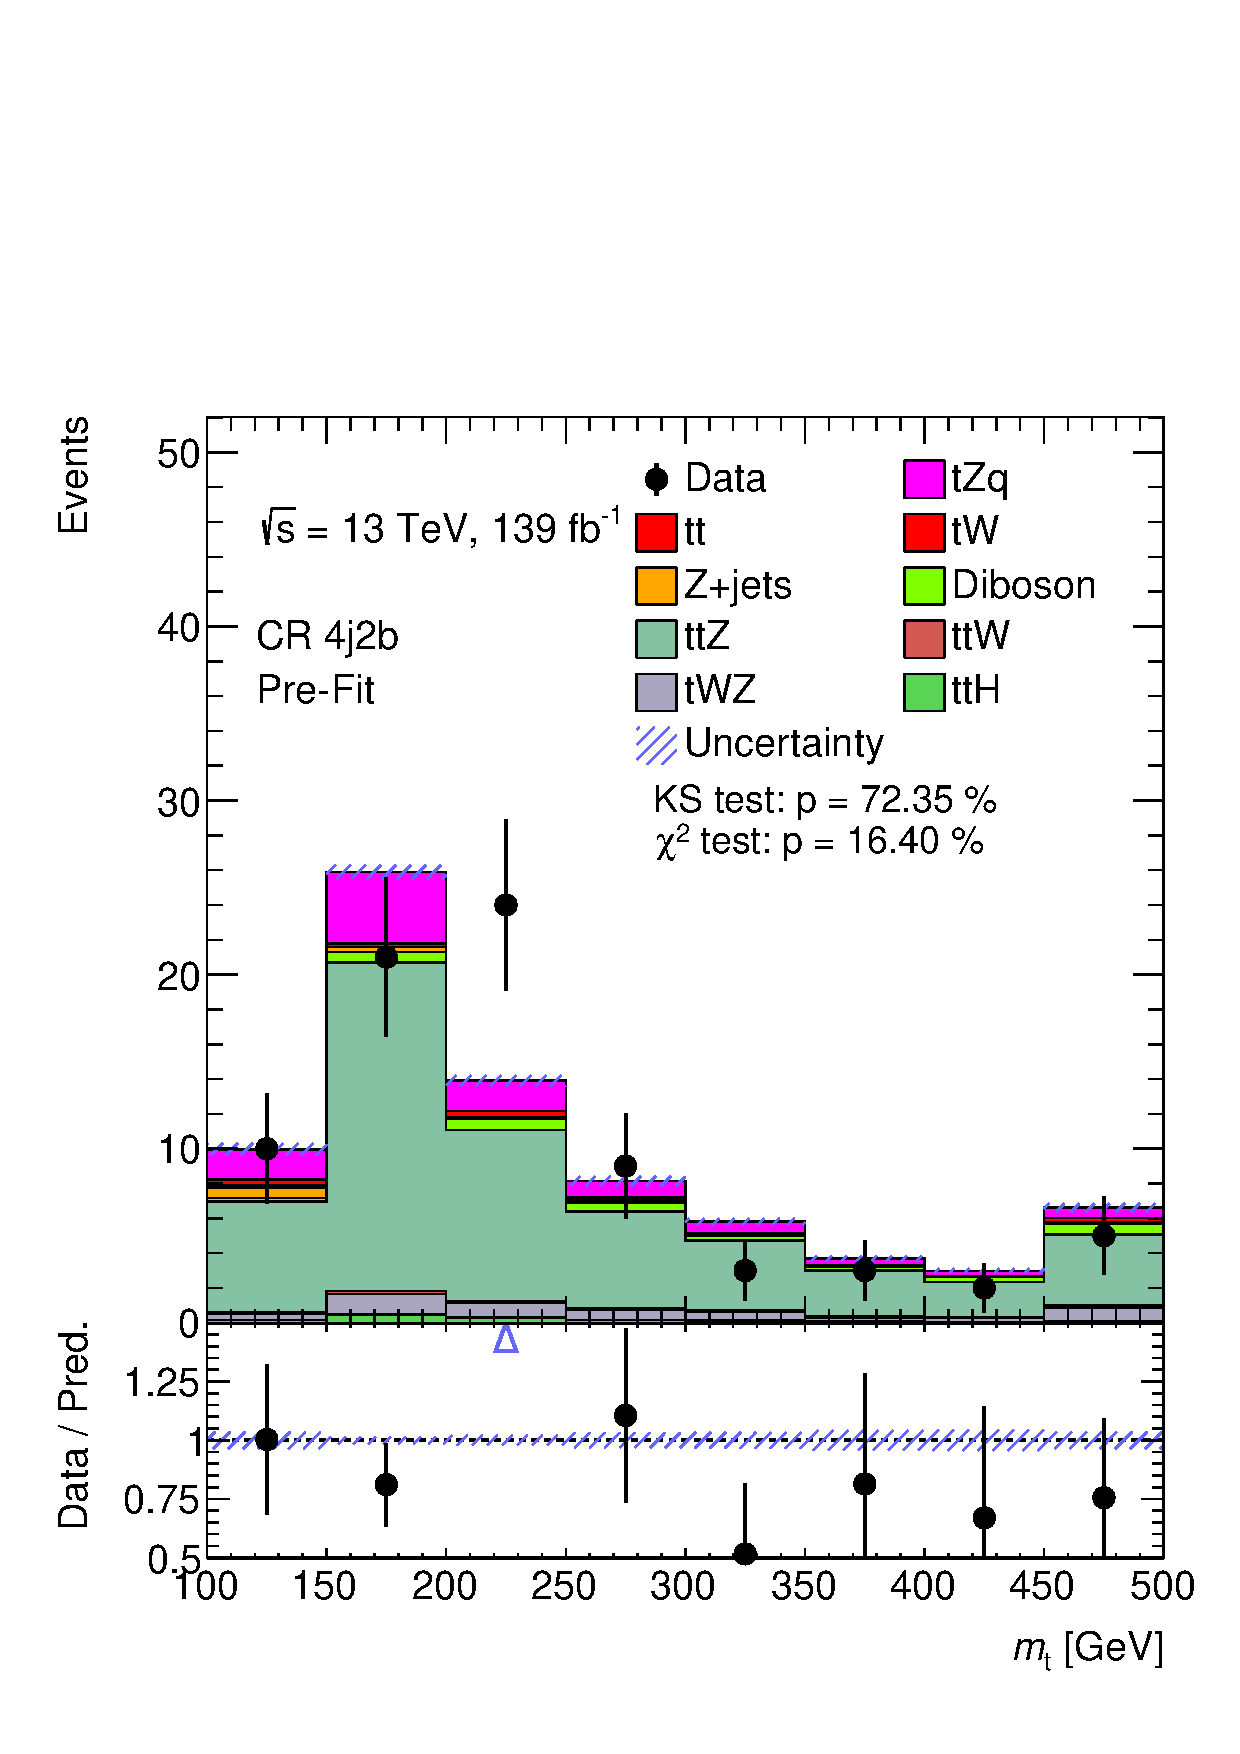
\includegraphics[width=\linewidth]{ubonn-thesis/Chapters/Chapters_05/Figure/CR_ttZ/CR_4j2b_Top_mass.pdf} 
  \end{subfigure}
  \caption{Comparison of data and MC predictions for reconstructed event- related quantities for events in the CR 3j2b and CR 4j2b. The uncertainty shown is the statistical uncertainty.}
  \label{fig:ttZ}
  \end{figure}



The two $t\Bar{t}Z$ control regions are listed in table \ref{tab:final_selection}. The events yields in $t\Bar{t}Z$ CRs after the full section are shown in table \ref{tab:yield_ttZ}. Some of the reconstructed variables in this control regions are shown in figure \ref{fig:ttZ}.

The $t\Bar{t}Z$ CRs are unique in that they require an extra b-jet which introduces an ambiguity in the event selection and reconstruction criteria. Here, only one of the b-jet is considered and other one is neglected. The forward jet is then selected as in section \ref{sec:SR}. The $t\Bar{t}Z$ CRs also have contamination from tZq signal events which can create a bias in the measurement. This is solved by fitting the neural-network output, $O_{NN}$ distribution (section \ref{sec:NN}) which shows seperation between the tZq and $t\Bar{t}Z$. This allows robust constraint of $t\Bar{t}Z$ modeling and also a slight boost to the overall measurement’s senstivity.


\subsection{$t\Bar{t}$ CRs plots and yields}
\label{subsec:tt_plot_yield}

Finally, the $t\Bar{t}$ contribution can be enhanced by requiring the OSSF lepton requirement be removed, effectively removing the requirement on the Z boson and opposite-sign, different-flavor (OSDF) leptons condition is imposed. This phase space is dominated by $t\Bar{t}$ events with a fake lepton and a b-jet. 

The two $t\Bar{t}$ CRs are also defined in table \ref{tab:final_selection}. The event yields in the $t\Bar{t}$ CRs after the full selection can be found in table \ref{tab:yield_ttbar} and reconstructed variables from the top quark and Z boson are given in figure \ref{fig:CR_tt}.

The $t\Bar{t}$ CRs suffer from the lowest statistics of all fitted regions. Because of this, two binned histograms per region is used in the statistical analysis.

\begin{table}[!h]
    \begin{minipage}{.49\textwidth}
      \centering
      \begin{adjustbox}{width=\textwidth}
       \begin{tabular}{@{} *3l @{}}
 \toprule
 Process & Number of events & Number of raw events  \\ [0.5ex] 
 \hline\hline
  tZq   &  0.34 \pm 0.04 & 200994 \\ 
  tt   &  43.40 \pm 1.23 & 197797 \\ 
  tW   & 2.32 \pm 0.52  & 3058 \\ 
  Z+jets   &  0.19 \pm 0.15 & 556  \\ 
  Diboson   & 0.39 \pm 0.07 & 21545 \\ 
  ttZ   & 2.69 \pm 0.12 & 262293 \\ 
  ttW   & 9.76 \pm 0.26 & 494284 \\ 
  tWZ   & 0.44 \pm 0.10  & 12649  \\ 
  ttH   &  3.35 \pm 0.05 & 1234180 \\ 
\hline 
  Total expected  & 62.87 \pm 1.37 & 2427360 \\ 
\hline 
  Data   & 71 & 71  \\ 
 \bottomrule
 \end{tabular} 
 \end{adjustbox}
    \end{minipage}%
    \hfill
    %\hspace{-1.5cm}
    \begin{minipage}{.50\textwidth}
      \centering
      \vspace*{0.5cm}
      \begin{adjustbox}{width=\textwidth}
        \begin{tabular}{@{} *3l @{}}
 \toprule
 Process & Number of events & Number of raw events  \\ [0.5ex] 
 \hline\hline
   tZq   & 0.21 \pm 0.03  & 139834  \\ 
  tt   & 20.27 \pm 0.84 &  93408 \\ 
  tW   & 1.06 \pm 0.61  & 1251 \\ 
  Z+jets & 0.13 \pm 0.13 &  417 \\ 
  Diboson  & 0.30 \pm 0.04 & 14178 \\ 
  ttZ   & 2.47 \pm 0.12 & 284950  \\ 
  ttW   & 5.19 \pm 0.20 & 308302  \\ 
  tWZ   & 0.26 \pm 0.09 & 10981 \\ 
  ttH   & 3.90 \pm 0.06  &  1.222370 \\ 
\hline 
  Total expected  & 33.80 \pm 0.96   & 2075690  \\ 
\hline 
  Data    & 49 & 49 \\ 
 \bottomrule
 \end{tabular} 
 \end{adjustbox}
    \end{minipage} 
    \caption{Numbers of expected events in the CR 2j1b (Left) and CR 3j1b (Right) broken down by process. The uncertainty shown contains only the statistical component.}
    \label{tab:yield_ttbar}
\end{table}


\begin{figure}[h!] 
  \begin{subfigure}[b]{0.33\linewidth}
    \centering
    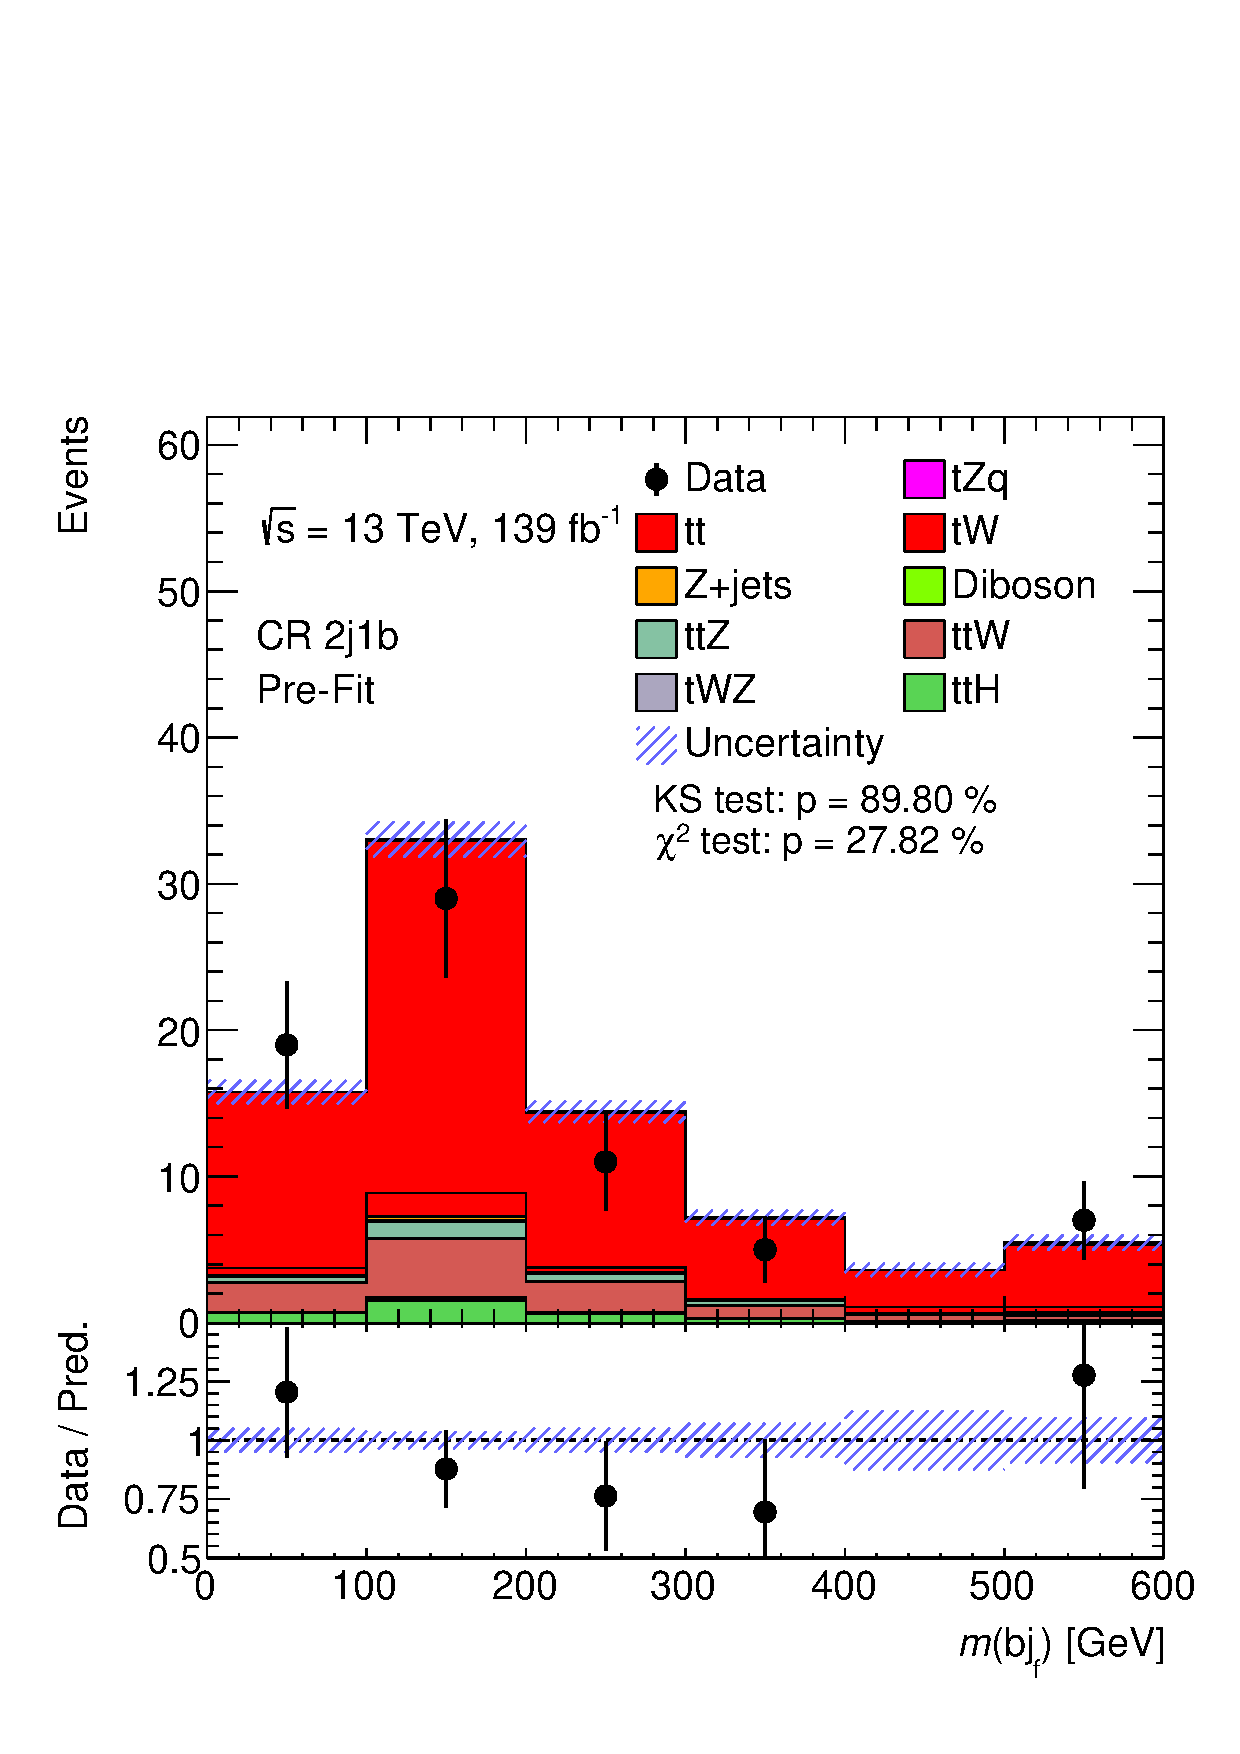
\includegraphics[width=\linewidth]{ubonn-thesis/Chapters/Chapters_05/Figure/CR_tt/CR_2j1b_M_bj.pdf} 
  \end{subfigure}%% 
  \begin{subfigure}[b]{0.33\linewidth}
    \centering
    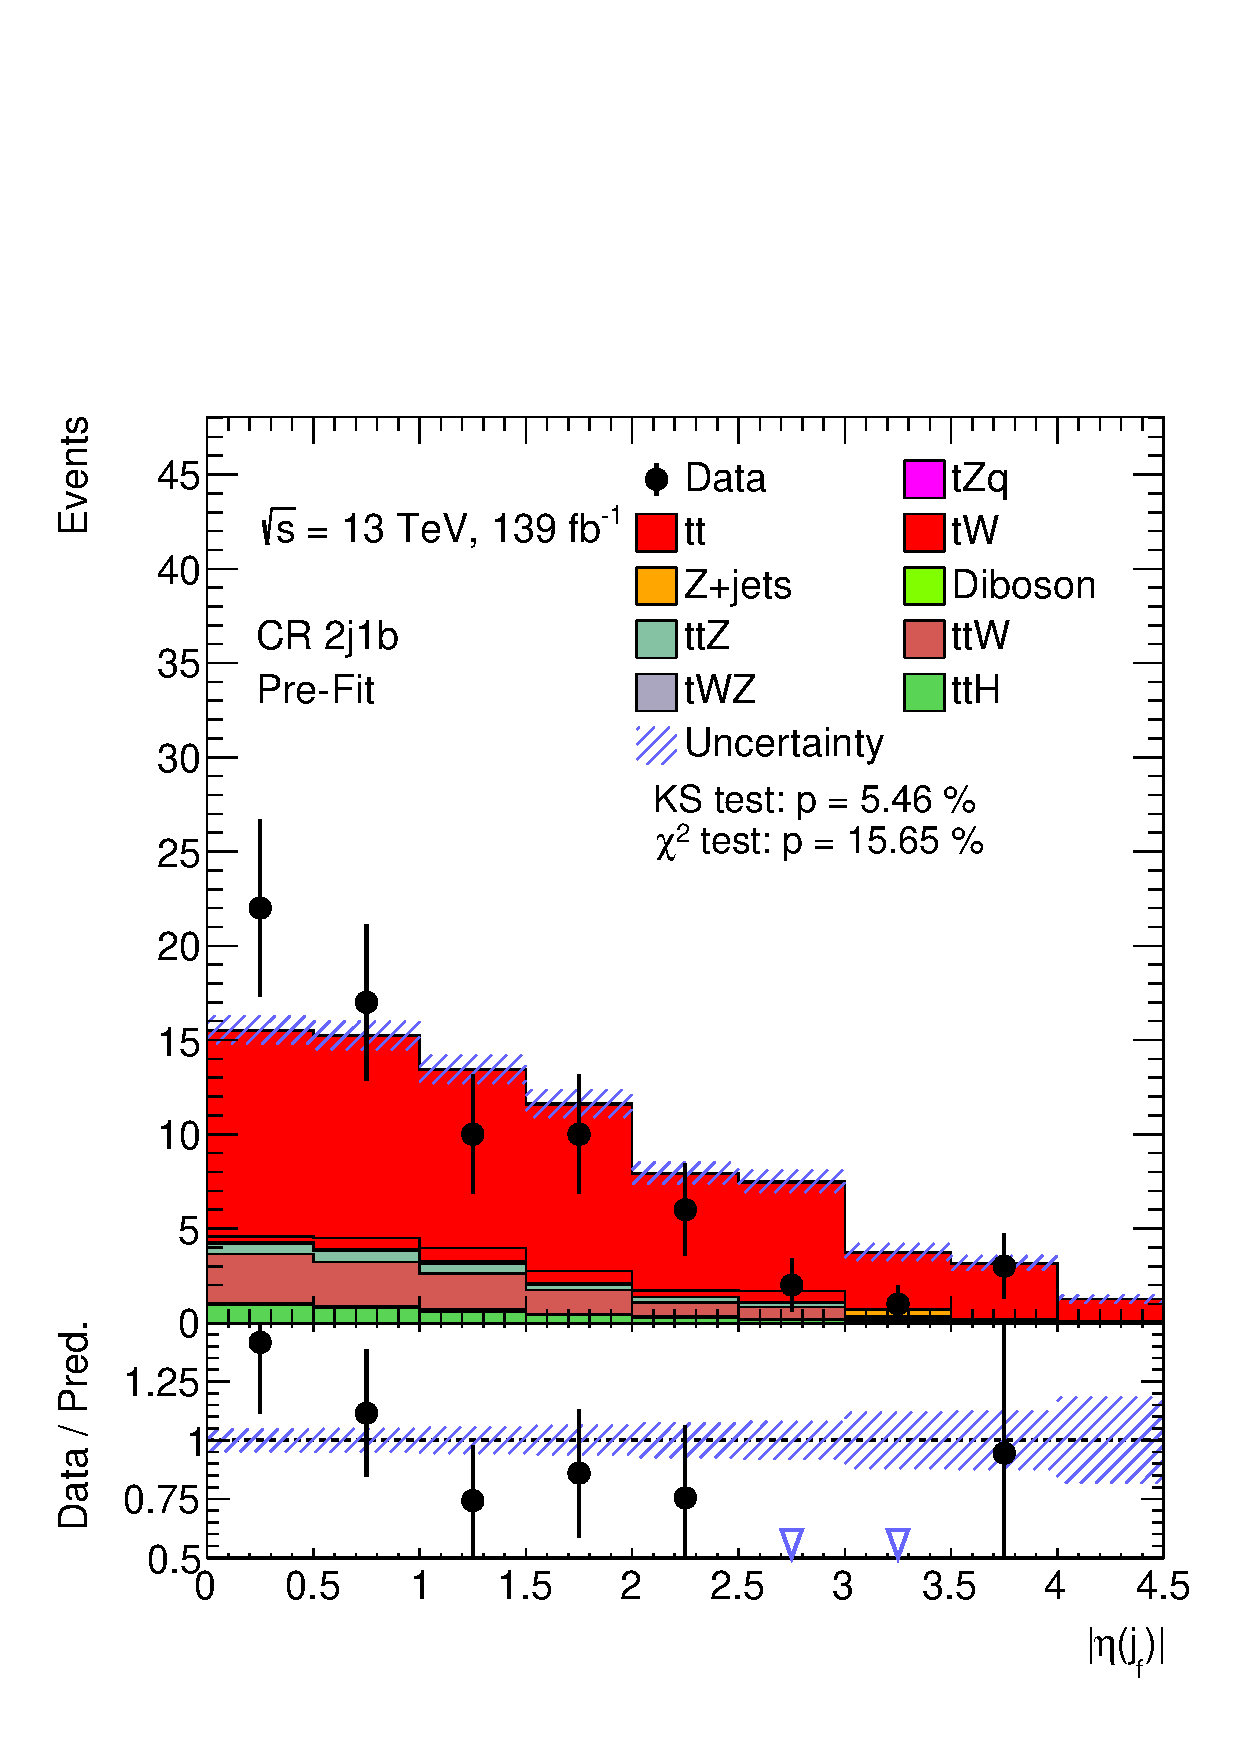
\includegraphics[width=\linewidth]{ubonn-thesis/Chapters/Chapters_05/Figure/CR_tt/CR_2j1b_forwardjet_eta.pdf} 
  \end{subfigure} 
  \begin{subfigure}[b]{0.33\linewidth}
    \centering
    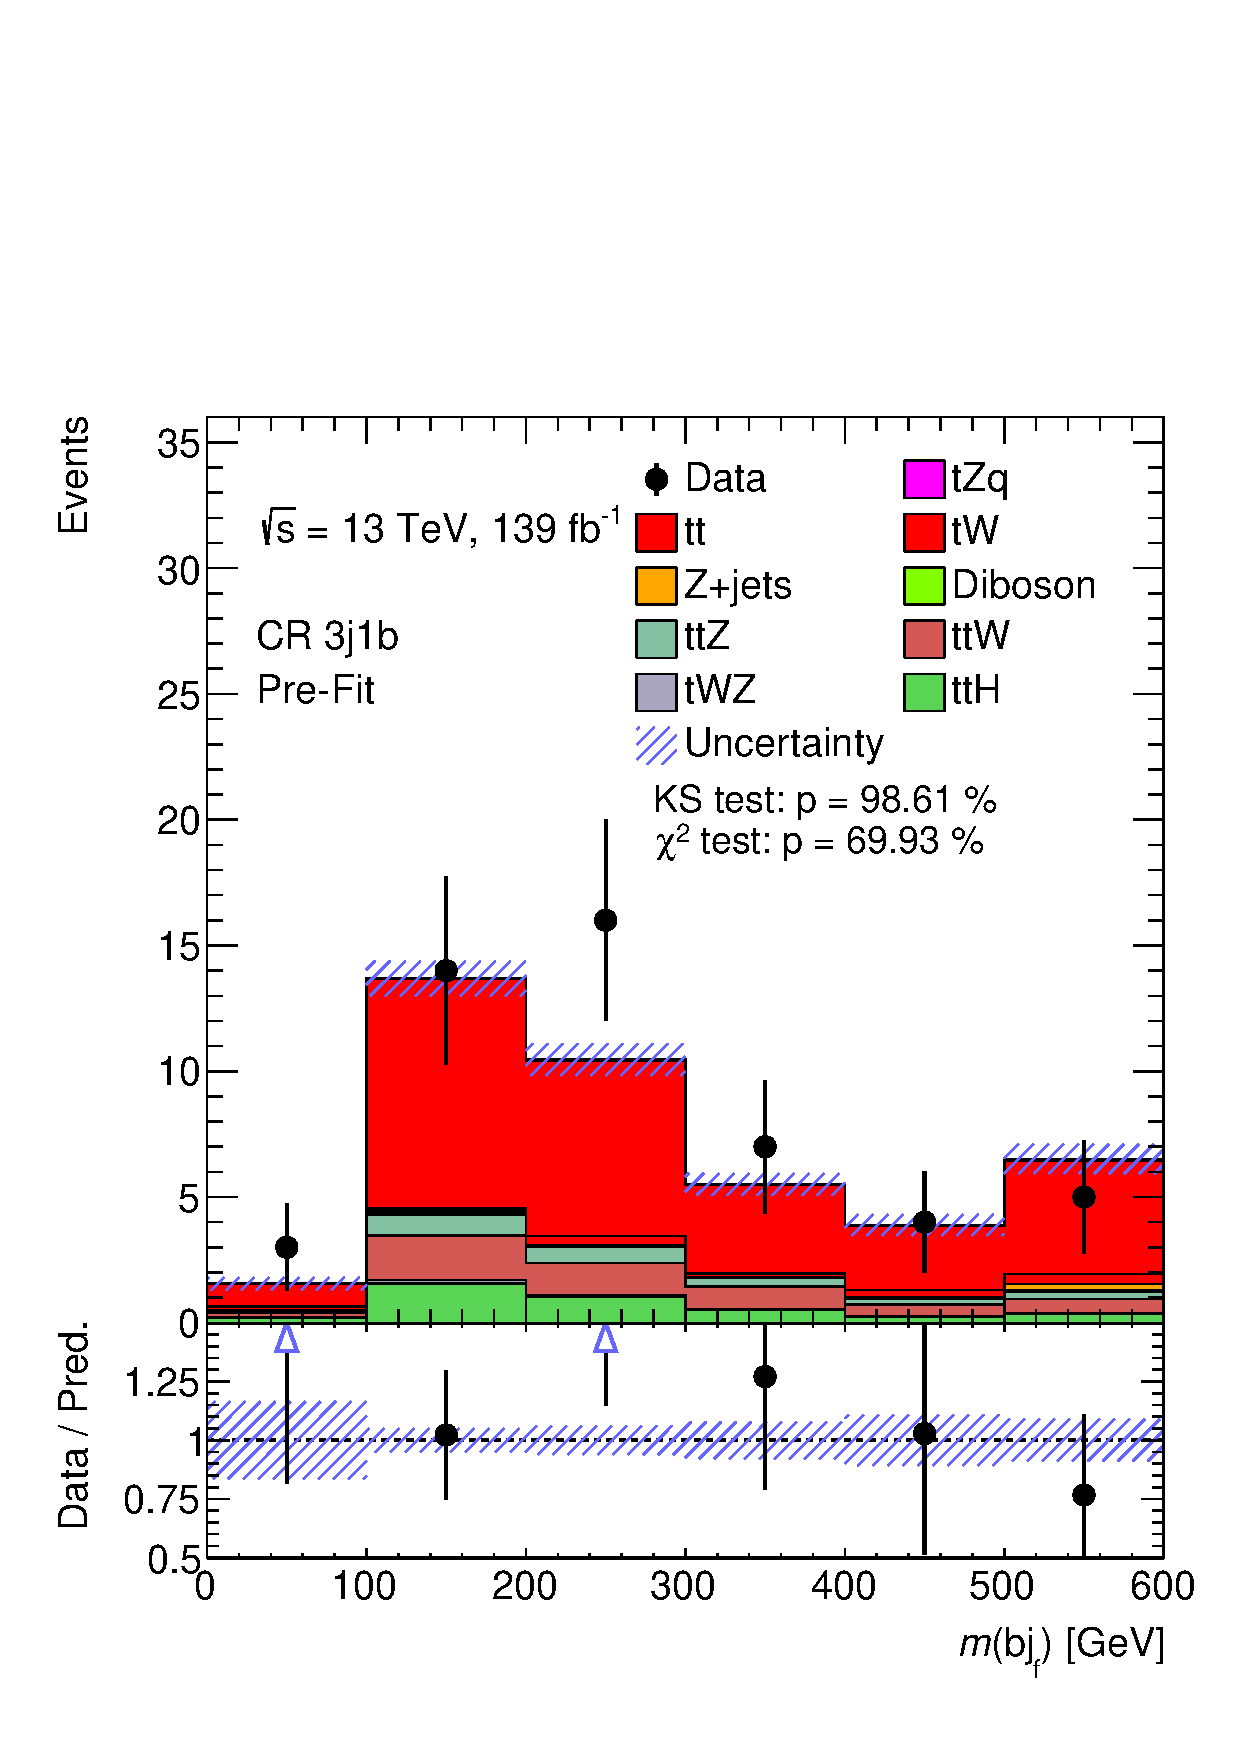
\includegraphics[width=\linewidth]{ubonn-thesis/Chapters/Chapters_05/Figure/CR_tt/CR_3j1b_M_bj.pdf} 
  \end{subfigure}%%
  \newline
  \begin{subfigure}[b]{0.33\linewidth}
    \centering
    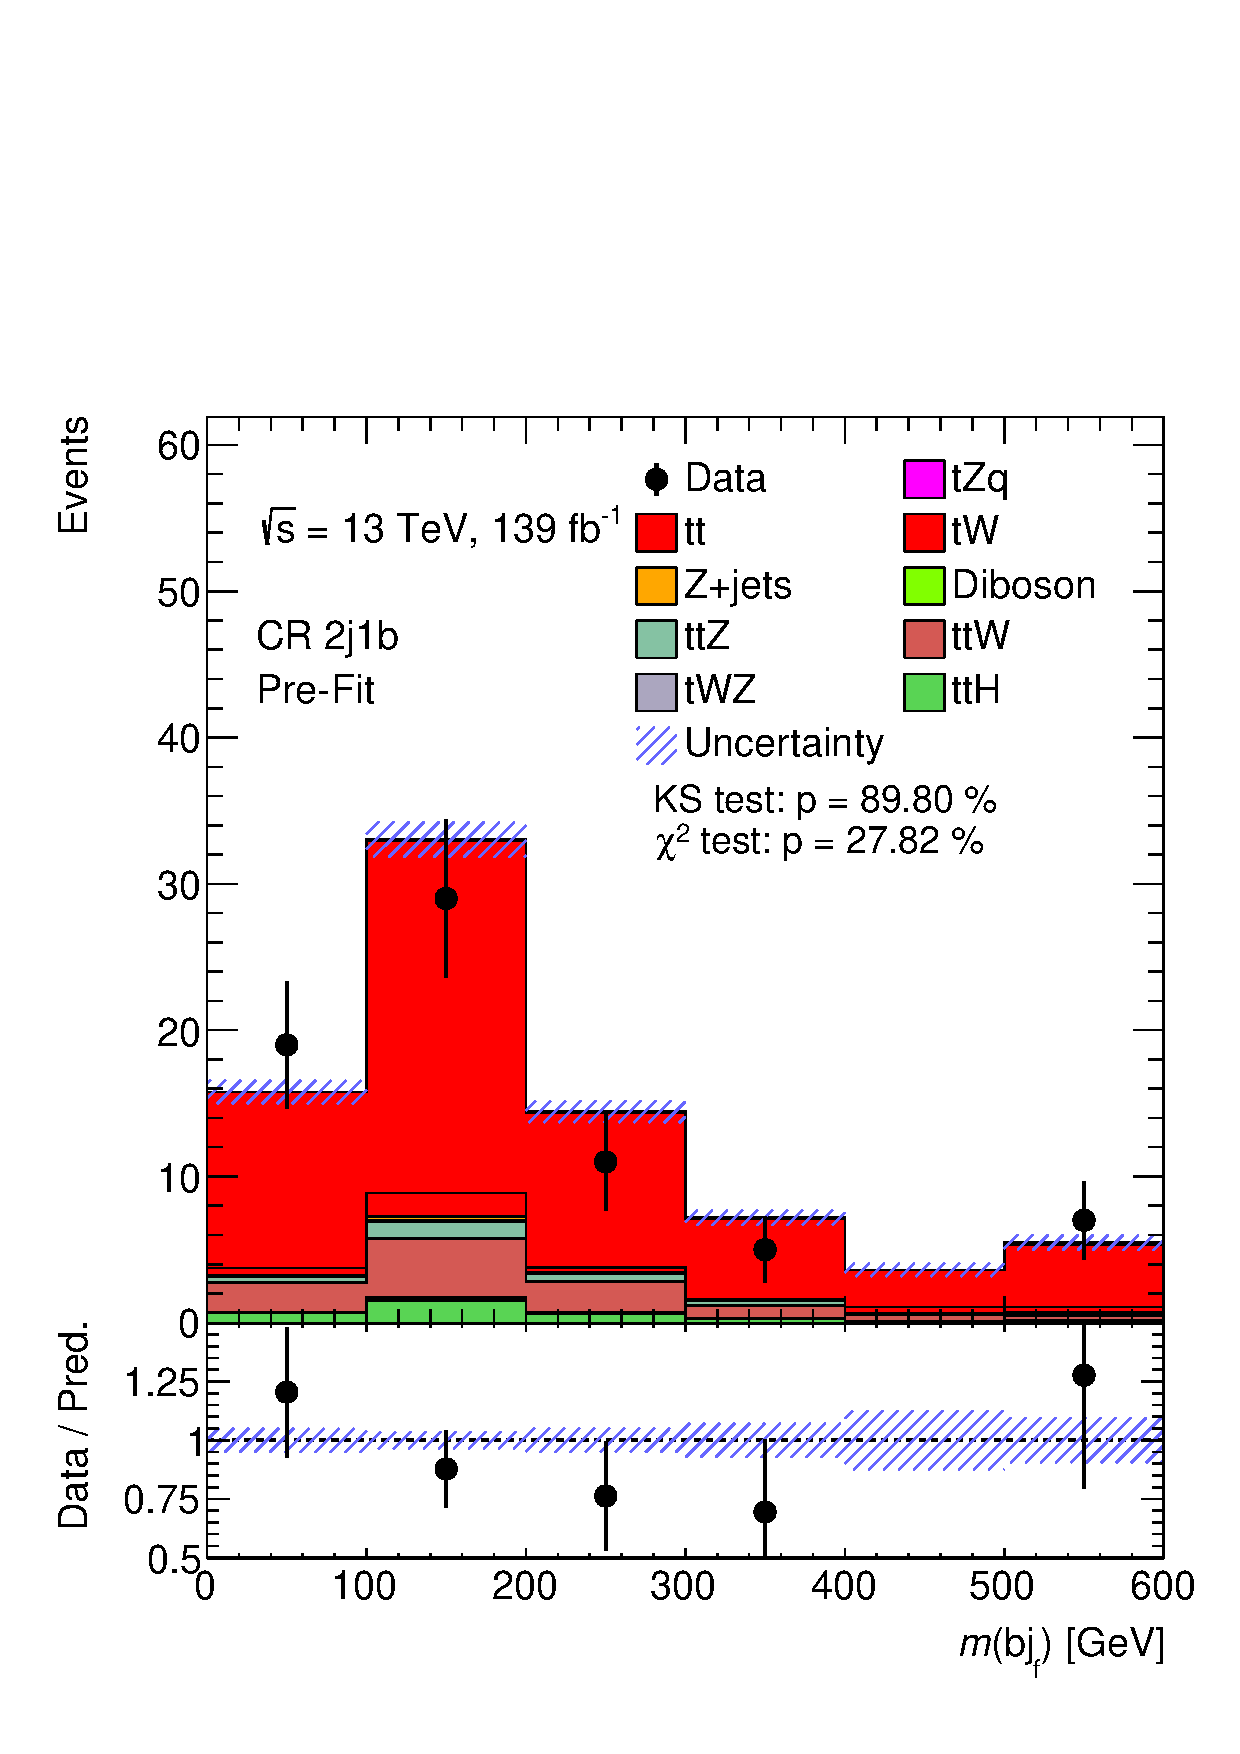
\includegraphics[width=\linewidth]{ubonn-thesis/Chapters/Chapters_05/Figure/CR_tt/CR_2j1b_M_bj.pdf} 
  \end{subfigure}%% 
  \begin{subfigure}[b]{0.33\linewidth}
    \centering
    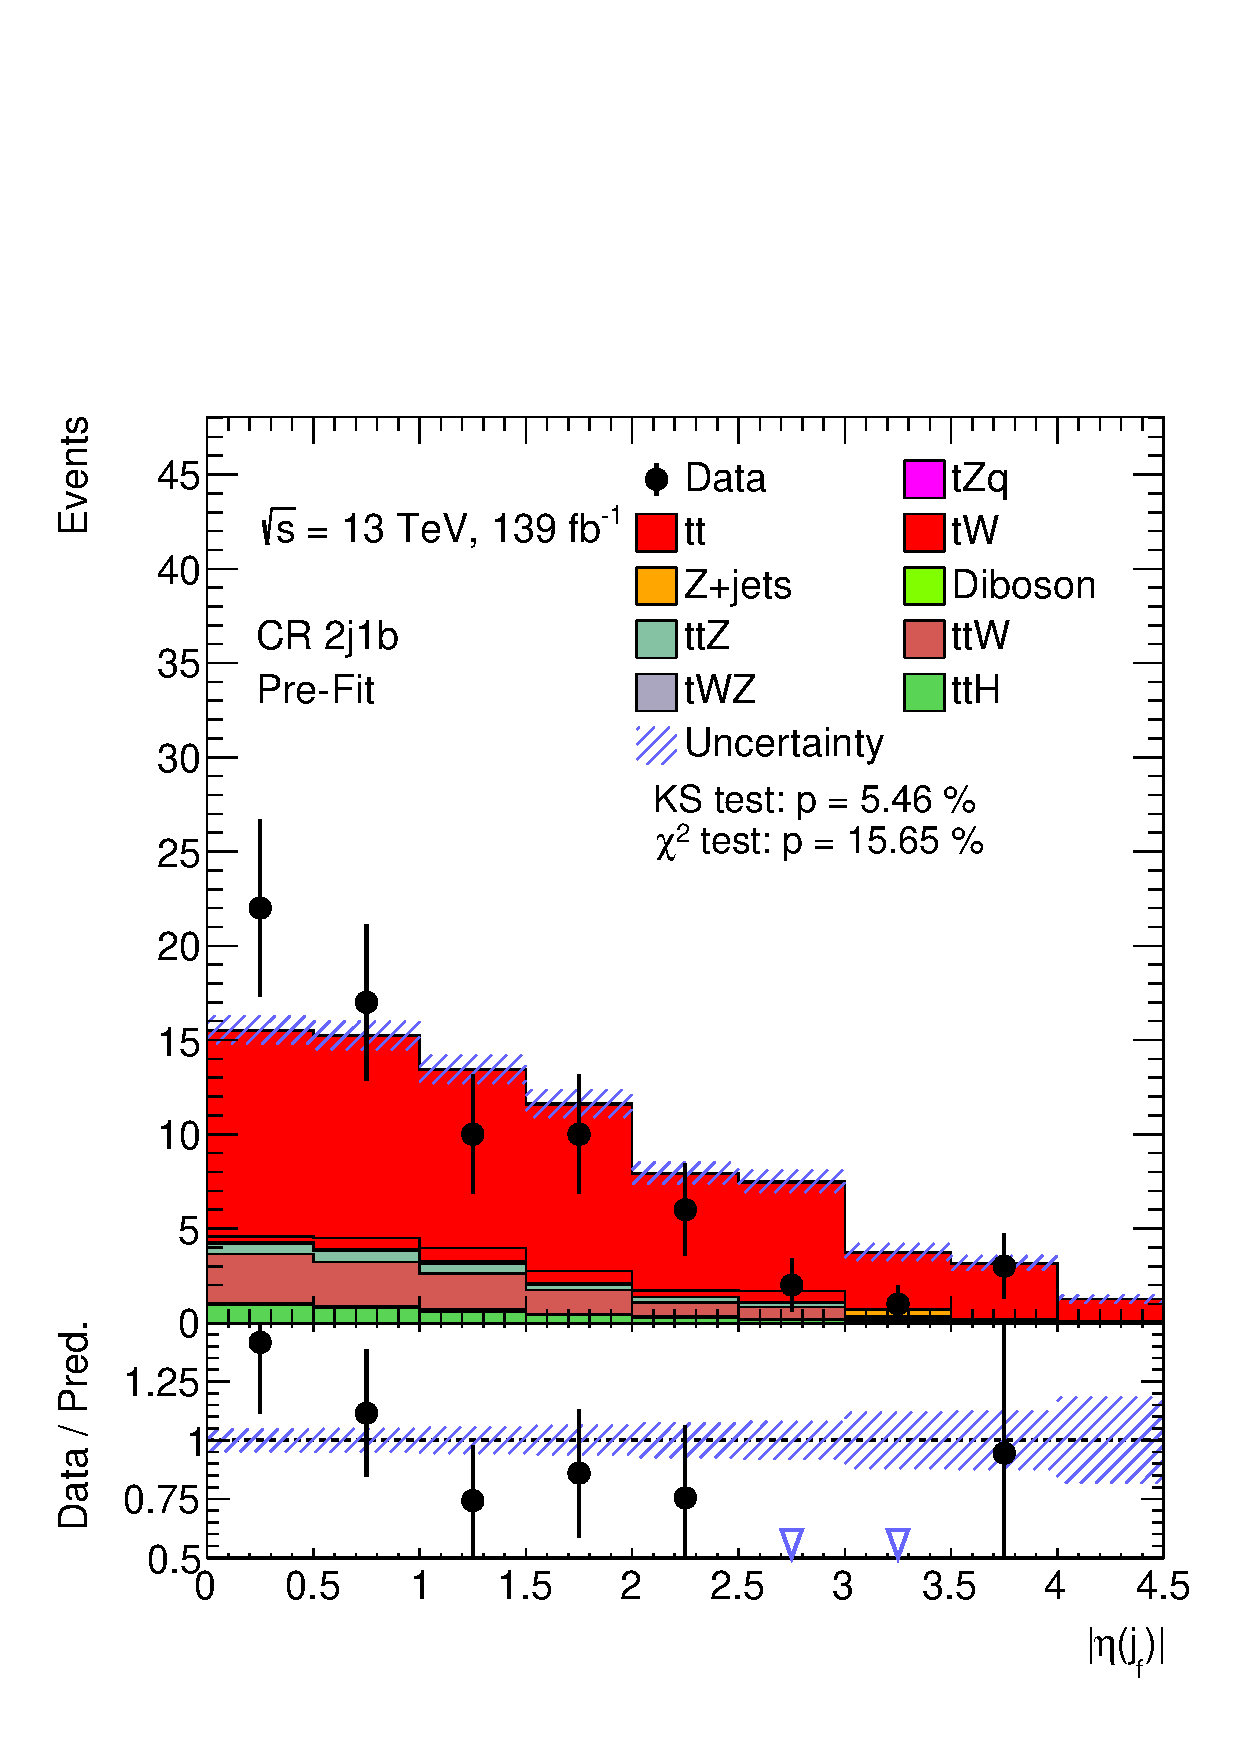
\includegraphics[width=\linewidth]{ubonn-thesis/Chapters/Chapters_05/Figure/CR_tt/CR_2j1b_forwardjet_eta.pdf} 
  \end{subfigure} 
  \begin{subfigure}[b]{0.33\linewidth}
    \centering
    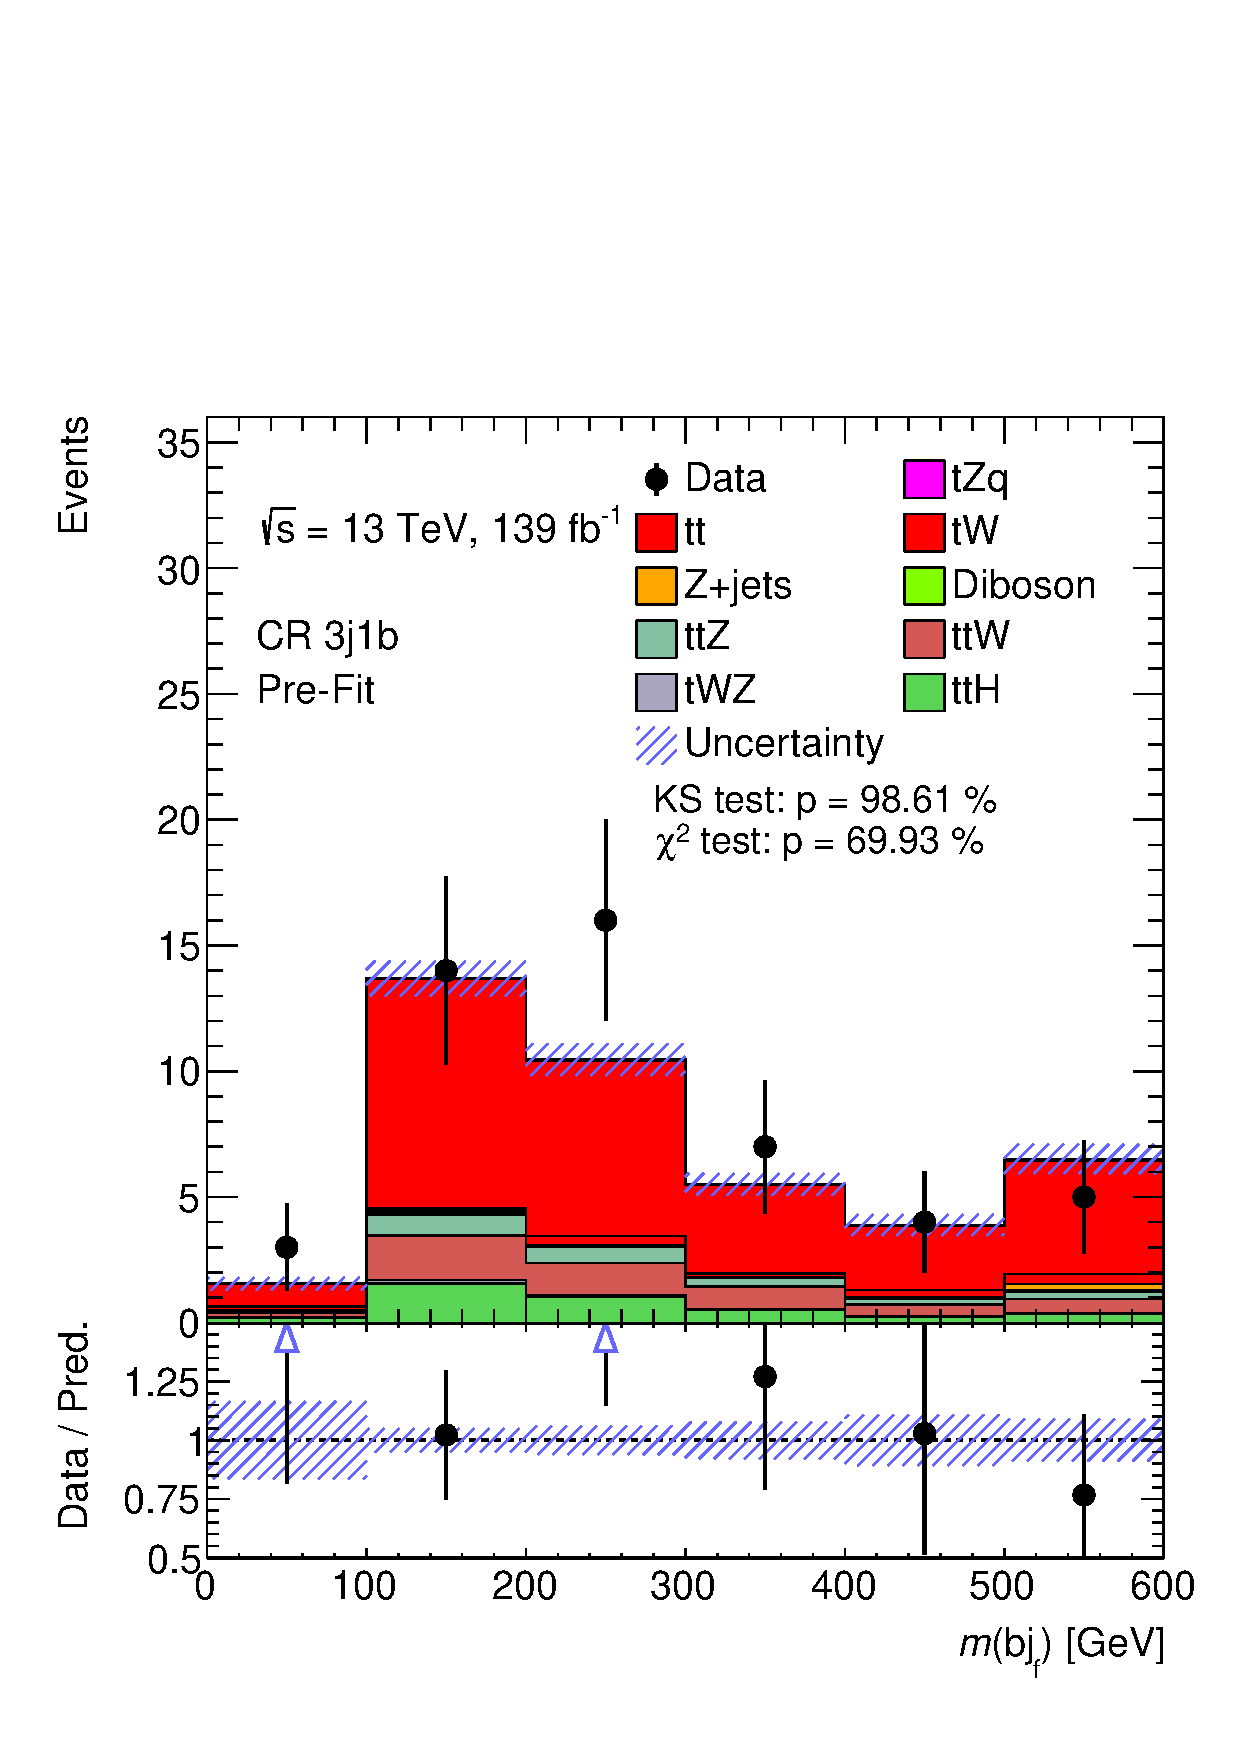
\includegraphics[width=\linewidth]{ubonn-thesis/Chapters/Chapters_05/Figure/CR_tt/CR_3j1b_M_bj.pdf} 
  \end{subfigure}%%
  \caption{Comparison of data and MC predictions for reconstructed event- related quantities for events in the CR 2j1b and CR 3j1b. The uncertainty shown is the statistical uncertainty.}
  \label{fig:CR_tt} 
  \end{figure}
  

%\begin{figure}[ht!] 
  
%\end{figure}
